\documentclass{article}
\usepackage{imakeidx} % Per creare un vero indice
%\usepackage{tcolorbox}
\usepackage{xcolor}
\usepackage[utf8]{inputenc}
\usepackage[T1]{fontenc}
\usepackage[italian]{babel}
\usepackage{multicol}
\usepackage{listings}
\usepackage{tikz}
\usepackage{hyperref} % Per l'aggiunta di link cliccabili
\usepackage{makecell}
\usepackage{pdfpages}
\usepackage{geometry}
\usepackage{array}
\usepackage{multirow, tabularx}
\usepackage{float}
\usepackage{colortbl}
\usepackage{graphicx} % Per l'inserimento di immagini

\def\arraystretch{1.5}
\renewcommand\theadalign{bc}
\renewcommand\theadfont{\bfseries}
\renewcommand\theadgape{\Gape[4pt]}
\newcolumntype{Y}{>{\centering\arraybackslash}X}

\lstdefinestyle{JavaStyle}{
	language=Java,
	basicstyle=\small\ttfamily,
	keywordstyle=\color{blue},
	commentstyle=\color{purple!40!black},
	stringstyle=\color{violet},
	breaklines=true,
	showstringspaces=false,
	tabsize=4,
	numbers=left,
	numberstyle=\tiny\color{gray},
	frame=single
}

\makeindex
\definecolor{dark_purple}{RGB}{48, 25, 52}

\begin{document}
	\begin{center}
		\textbf{UNIVERSITÀ DEGLI STUDI DI NAPOLI \\ FEDERICO II}
		\\
		\vspace{1cm}
		
\includegraphics[width=0.2\textwidth]{Immagini/logo_universita.png} 
	\end{center}
	
	\vspace{1cm}
	
	\begin{center}
		\textbf{Corso di Ingegneria del Software} \\
		\vspace{0.5cm}
		\textbf{DIPARTIMENTO DI INGEGNERIA ELETTRICA E TECNOLOGIE DELL'INFORMAZIONE} \\
		\vspace{0.5cm}
		
\includegraphics[width=0.6\textwidth]{Immagini/logo_sfondo} \\
		\textbf{\textcolor{dark_purple}{Enjoy music, enjoy the lab}}
		
	\end{center}
	
	\vspace{0.5cm}
	
	\begin{center}
		\textbf{Candidati:} \\
		Fabrizio Di Giovanni - N8600- \\
		Lucia Brando - N86003382 \\
		Dario Morace - N8600- \\
		ID GRUPPO:- - - - -\\
	\end{center}
	
	\vspace{0.5cm}
	
	\begin{center}
		\textbf{Docenti:} \\
		Prof. Sergio Di Martino \\
		Prof. Francesco Cutugno
	\end{center}
	
	\vspace{0.5cm}
	
	\begin{center}
		\textbf{ANNO ACCADEMICO 2023/2024}
	\end{center}
	

	\renewcommand{\contentsname}{Indice} % Rinomina la tabella dei contenuti
	\tableofcontents % Genera la tabella dei contenuti
	
	\clearpage
	
	\section{Introduzione}
	Si vuole realizzare, dietro commissione della società SoftEngUniNA, una piattaforma per gli appassionati di musica
	Nello specifico, la società ha richiesto la progettazione e implementazione di un applicativo mobile, oltre alla parziale verifica dei moduli necessari per il suo corretto funzionamento.
	Nasce così \textbf{\textit{\textcolor{dark_purple}{SoundLab}}}, un nuovo spazio dedicato a tutti coloro che fanno della musica la colonna portante delle loro giornate.
		\subsection{Che cos'è SoundLab}
		SoundLab è un servizio dedicato agli appassionati di musica, offrendo una vasta selezione di brani e generi musicali per soddisfare i gusti di tutti gli utenti registrati. Gli utenti possono accedere al sistema per esplorare e ascoltare musica, creare e gestire le proprie playlist, visibili sui loro profili personali. \\Inoltre, gli amministratori hanno accesso a strumenti di analisi avanzati, permettendo loro di visualizzare le statistiche relative ai brani e agli utenti presenti nel sistema, migliorando così l'esperienza complessiva degli utenti.
		\\
		\begin{figure}[H]
			\centering
			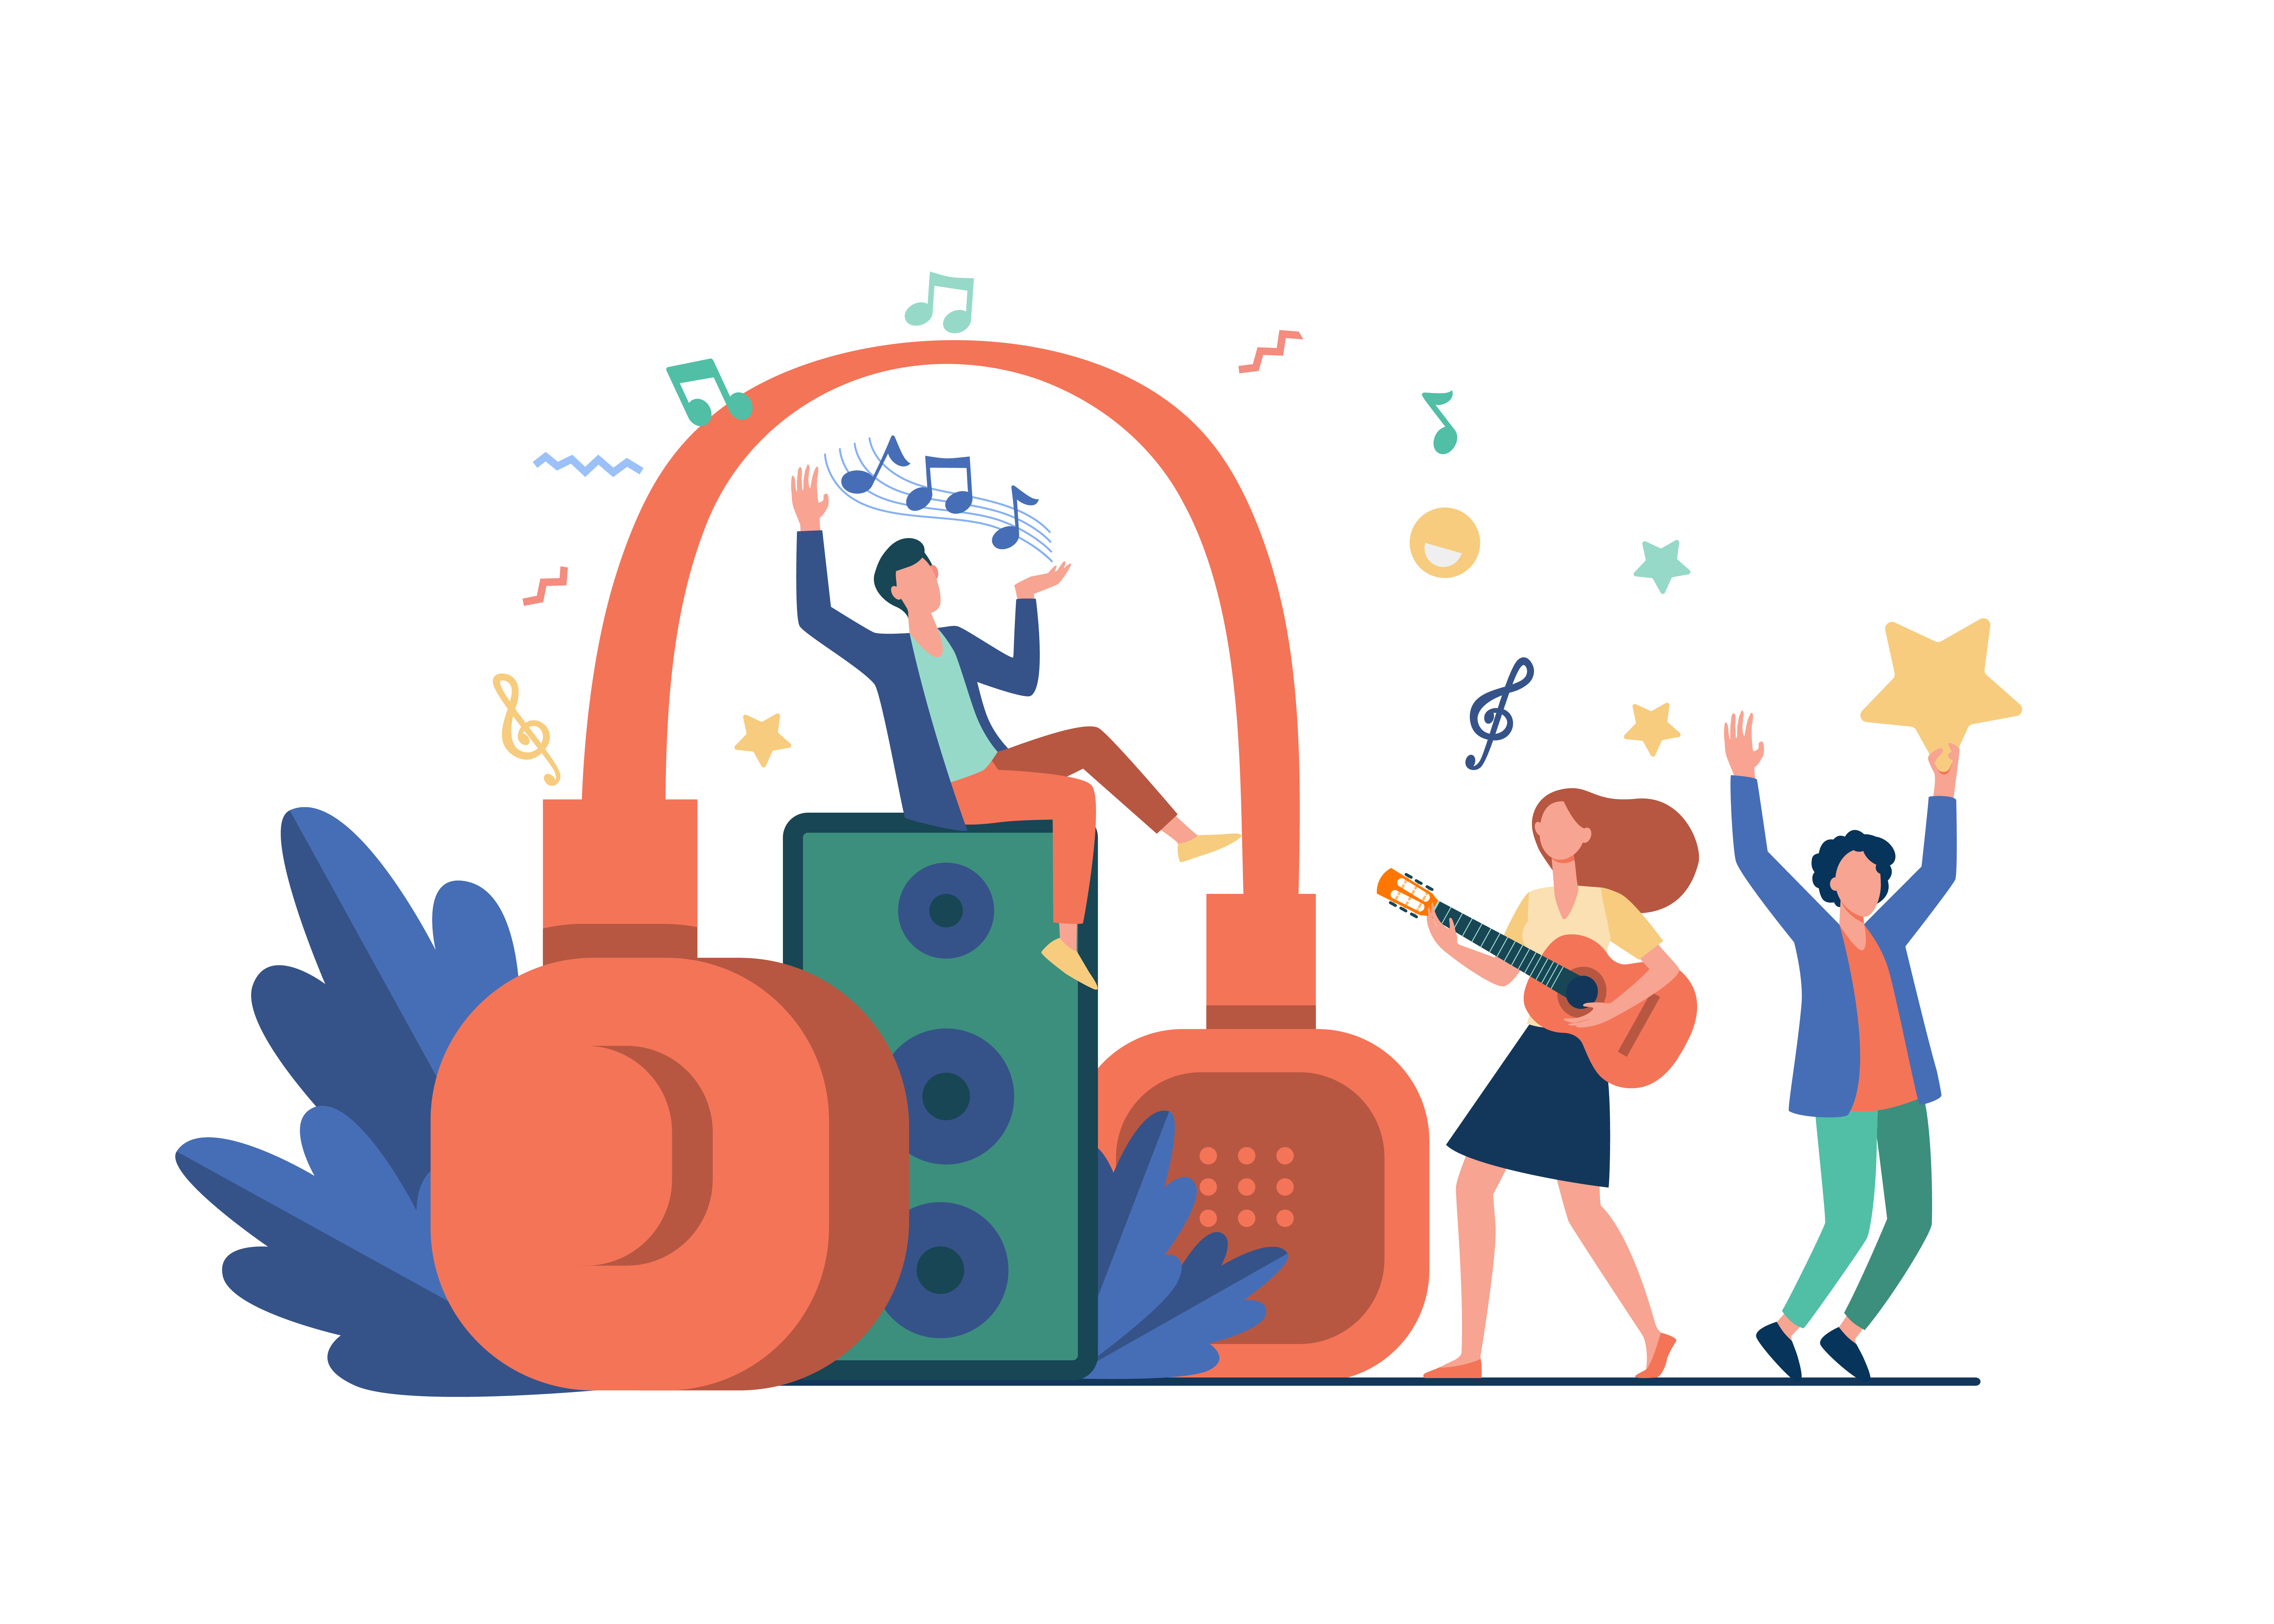
\includegraphics[width=0.9\textwidth]{Immagini/5870}
		\end{figure}
		In conformità con i recenti standard previsti dall’Unione Europea, Soundlab si impegna all’assoluto rispetto della privacy e dei dati della propria utenza per assicurare un’esperienza di navigazione sicura; proprio perché abbiamo a cuore tale sicurezza, il nostro staff si impegna a offre un’assistenza a 360 gradi.
		\subsection{Cosa offre Soundlab}
		Per offrire un'esperienza ottimale, SoundLab si basa su un robusto \textbf{\textit{\textcolor{dark_purple}{back-end}}} progettato per garantire prestazioni elevate e scalabilità in base alle esigenze dell'utenza. Questo sistema back-end avanzato assicura che l'applicazione possa gestire efficacemente un numero crescente di utenti e richieste, mantenendo sempre una risposta rapida e affidabile.\\
		Dall'altro lato, Soundlab presenta un'interfaccia \textbf{\textit{\textcolor{dark_purple}{front-end}}} semplice e moderna, progettata per rendere intuitiva la navigazione. Gli utenti possono facilmente cercare, esplorare e interagire con contenuti e funzionalità dell'applicazione, rendendo la loro esperienza unica e adattabile alle loro preferenze personali.\\ 
		La combinazione di un back-end potente e un'interfaccia utente intuitiva permette a SoundLab di offrire un servizio eccezionale, migliorando la soddisfazione degli utenti e favorendo un'interazione più profonda con la piattaforma.
		\subsection{Tecnologie utilizzate}
		L'applicativo è sviluppato interamente su piattaforma \textbf{\textit{\textcolor{dark_purple}{Android}}} utilizzando il linguaggio di programmazione \textbf{\textit{\textcolor{dark_purple}{Object-Oriented}}}, in particolare \textbf{\textit{\textcolor{dark_purple}{Java}}}.\\
		Questa scelta tecnologica garantisce robustezza, flessibilità e una vasta compatibilità con dispositivi Android di diverse generazioni. Inoltre, l'applicazione è dotata di un sistema di logging avanzato che facilita il testing efficace e la risoluzione rapida dei problemi, migliorando la qualità complessiva del software e l'esperienza utente.\\
		Per il back-end, SoundLab sfrutta tecnologie all'avanguardia, tra cui servizi di \textit{public Cloud Computing} che permettono di massimizzare la scalabilità e le prestazioni del sistema. Questi servizi cloud offrono una piattaforma affidabile e sicura per la gestione dei dati, consentendo al sistema di adattarsi dinamicamente al crescente numero di utenti e alle richieste variabili. La combinazione di un'applicazione front-end potente e intuitiva con un back-end scalabile e performante garantisce un servizio eccellente e un'esperienza utente ottimale.
		\\
		\\
		Nei capitoli successivi, approfondiremo ulteriormente il discorso sulle tecnologie utilizzate e forniremo, come richiesto da SoftEngUniNa, i documenti relativi al lavoro svolto per la realizzazione del progetto.
	\section{Modello Funzionale}
	In questa sezione andremo a descrivere il modello funzionale del software partendo da un'analisi dei casi d'uso assegnati per l'applicativo.
		\subsection{Requisiti dell'applicazione}
		\begin{tabular}{|p{6cm}|p{8cm}|}
			\hline
			\cellcolor{dark_purple}\textcolor{white}{\textbf{Funzionalità}} & \cellcolor{dark_purple}\textcolor{white}{\textbf{Descrizione}} \\
			\hline
			\textbf{Ricerca delle tracce musicali e/o artista} & Ricerca tramite nome una traccia musicale oppure un'artista all'interno della piattaforma. \\
			\hline
			\textbf{Gestione playlist} & L'utente ha la possibilità di creare, eliminare ed aggiungere/rimuovere una playlist dalle preferite. \\
			\hline
			\textbf{Visualizzazione profilo} & L'utente, in quanto iscritto, alla piattaforma può visualizzare il proprio profilo dove trova le playlist create e preferite. \\
			\hline
			\textbf{Gestione profilo} & L'utente, in quanto iscritto alla piattaforma, tramite i settings può gestire il proprio profilo. Si può: modificare l'username, modificare l'email, modificare la password, cancellare il proprio profilo o fare un semplice logout. \\
			\hline
			\textbf{Gestione delle tracce musicali} & L'utente può aggiungere e/o rimuovere una traccia musicale da una playlist. \\
			\hline
			\textbf{Visualizzazione statistiche (solo per l'utente admin)} & Tramite un'apposito bottone presente sul proprio profilo, l'admin può recuperare informazioni riguardo gli utenti, le fasce orarie in cui l'applicativo viene utilizzato e gli ascolti che effettuano. \\
			\hline
		\end{tabular}
			\subsubsection{Non funzionali}
			\begin{tabular}{|p{6cm}|p{8cm}|}
				\hline
				\cellcolor{dark_purple}\textcolor{white}{\textbf{Funzionalità}} & \cellcolor{dark_purple}\textcolor{white}{\textbf{Descrizione}} \\
				\hline
				\textbf{Usabilità} & L'applicazione deve presentarsi in modo semplice, cosi da permettere ad ogni tipologia di utente di fare uso di tutte le funzionalità che essa mette a disposizione. \\
				\hline
				\textbf{Scalabilità} & Il sistema deve potersi adattare ai cambiamenti del backend, in modo da garantire la manutenibilità nel tempo. \\
				\hline
				\textbf{Password policy security} & Le password verranno salvate con un controllo regex avanzato. \\
				\hline
				\textbf{Prestazioni} & Il sistema deve essere utilizzabile entro 3 secondi dall’avvio. Inoltre,non devono presentarsi rallentamenti che impediscano all’utente di effettuareoperazioni. \\
				\hline
				\textbf{Utilizzo di single-activity e multi-fragment} & L’applicazione utilizza perfluidità e facile gestione il pattern di single-activity e multi-fragment in mododa dare precisi scopi alle activity che gestiscono fragment comuni. \\
				\hline
			\end{tabular}
			\subsubsection{Dominio}
			\begin{tabular}{|p{6cm}|p{8cm}|}
				\hline
				\cellcolor{dark_purple}\textcolor{white}{\textbf{Dominio}} & \cellcolor{dark_purple}\textcolor{white}{\textbf{Descrizione}} \\
				\hline
				\textbf{General Data Protection Regulation} & Il sistema deve essere conforme al Regolamento Generale sullaProtezione dei Dati (GDPR), incentrato sul trattamento dei dati personali e sulla privacydell’utente \\
				\hline
				\textbf{ISO/IEC 27018:2019} & Il sistema deve essere conforme allo standard ISO/IEC 27018:2019[9],incentrato sulla protezione dei dati personali nel cloud. \\
				\hline
				\end{tabular}
				\newpage
		\subsection{Modellazione degli Use Case}
		Per la documentazione dei casi d'uso è stato utilizzato un software case tool, chiamato Visual Paradigm.\\
		Per fini di visibilità e leggibilità dei singoli use case, si è deciso di modellare il diagramma in package.
			\subsubsection{Caso generale}
			Il seguente use case rappresenta l'insieme delle funzionalità del sistema assegnate dalla software house.
				\begin{figure}[H]
					\centering
					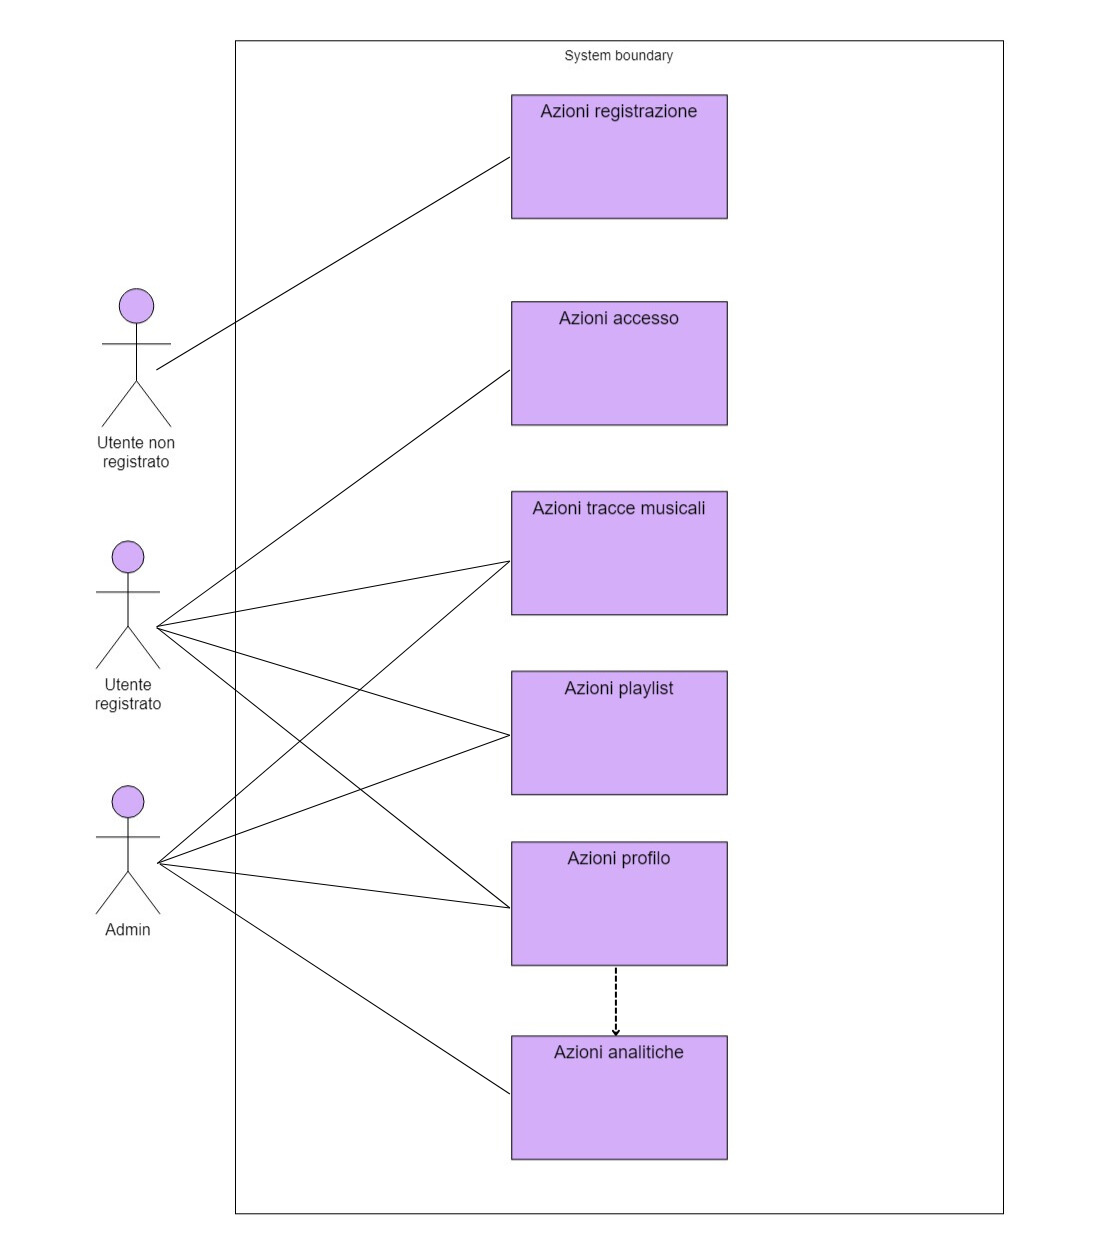
\includegraphics[width=0.8\textwidth]{Immagini/usecasegenerale.png}
					\caption{Use Case Diagram generale}
				\end{figure}
				
			\subsubsection{Use Case azioni playlist}
			Nella seguente figura è descritto l'insieme delle azioni riguardanti le playlist.\\
			Si identificano le seguenti:
			\begin{itemize}
				\item Creare una nuova playlist
				\item Aggiungere un brano alla playlist
				\item Rimuovere un brano dalla playlist
				\item Rinominare una playlist
				\item Cambiare genere ad una playlist
				\item Aggiungere e/o rimuovere una playlist dalle preferite
				\item Eliminare una playlist
			\end{itemize}
			
			\begin{figure}[H]
				\centering
				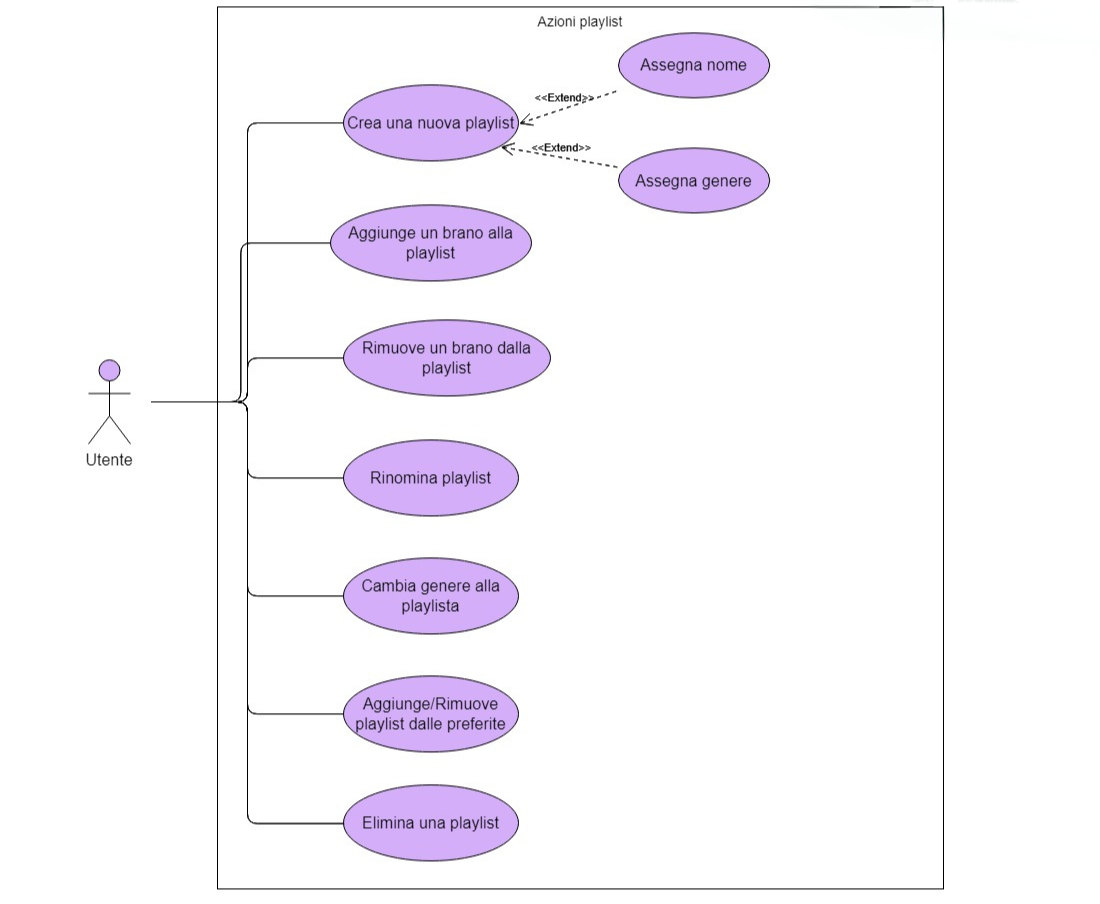
\includegraphics[width=0.9\textwidth]{Immagini/Funzioniplaylist.png}
				\caption{Use Case Diagram azioni playlist}
			\end{figure}
			\subsubsection{Use Case aggiunta playlist ai preferiti}
			Nella seguente figura viene illustrato nel dettaglio il processo di aggiunta/rimozione di una playlist ai preferiti. L'utente, mediante l'utilizzo di un apposito toggle, può scegliere di includere o escludere tale playlist dall'elenco dei preferiti.
			
			\begin{figure}[H]
				\centering
				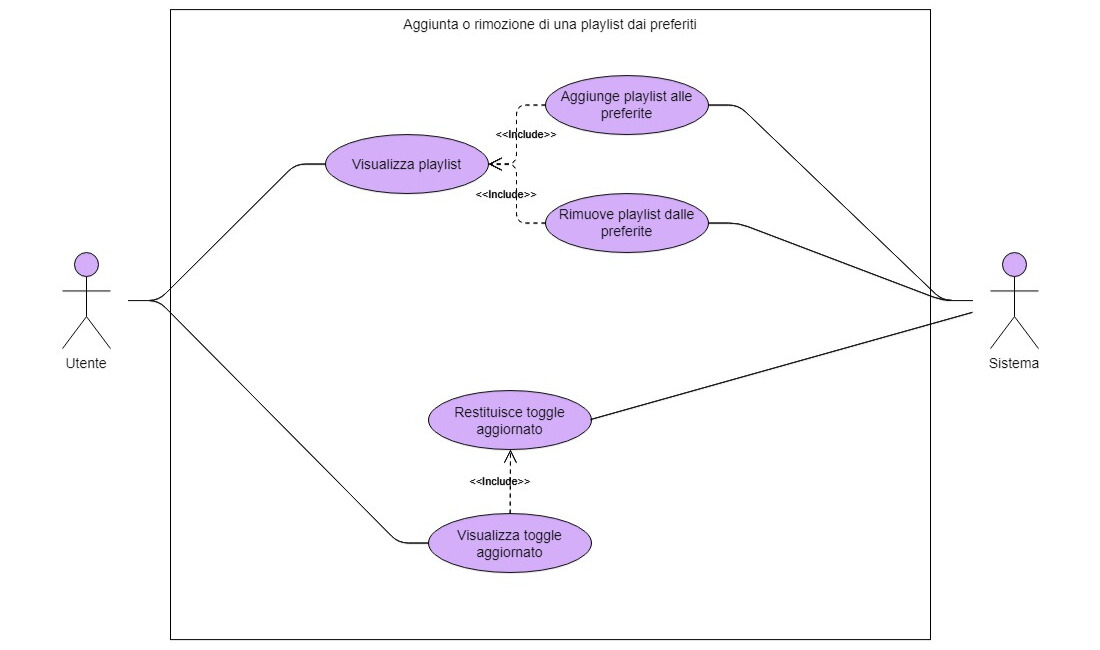
\includegraphics[width=0.9\textwidth]{Immagini/aggiuntarimozione.png}
				\caption{Use Case Diagram aggiunta/rimozione playlist dai preferiti}
			\end{figure}
			\newpage
			\subsubsection{Use Case aggiunta brano dalla playlist}
			Nella seguente figura si è scelto di mostrare nel dettaglio l'aggiunta di una traccia musicale da una playlist.
			
			\begin{figure}[H]
				\centering
				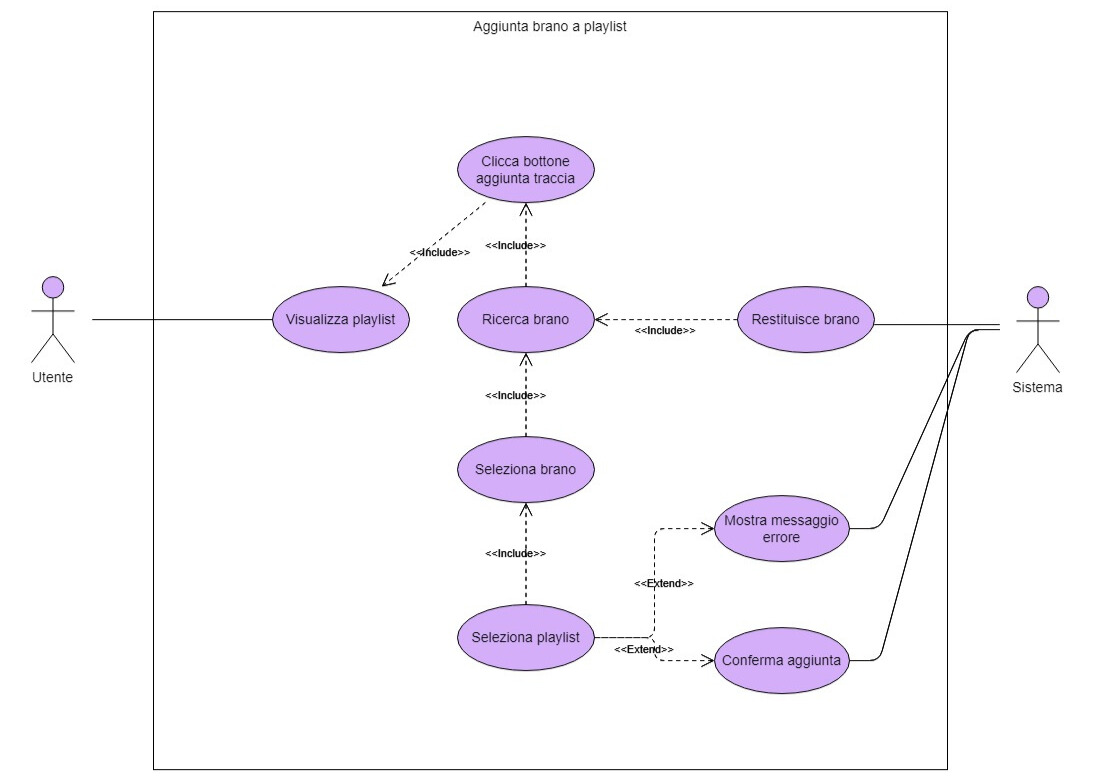
\includegraphics[width=0.9\textwidth]{Immagini/aggiuntatraccia.png}
				\caption{Use Case Diagram aggiunta traccia musicale ad una playlist}
			\end{figure}
			
			\subsubsection{Use Case azioni analitiche}
			Il seguente use case rappresenta l'insieme di azioni che solamente l'utente admin può compiere.\\
			Le azioni in questione riguardano le analitiche:
			\begin{itemize}
				\item Se l'admin ricerca un utente, egli visualizzerà \textit{il numero di ascolti compiuti e la fascia oraria in cui ha utilizzato di più la piattaforma.}
				\item Se l'admin ricerca una traccia musicale, egli visualizzerà \textit{la tipologia della canzone, l'artista e il numero di ascolti totali del brano.}
				
				\begin{figure}[H]
					\centering
					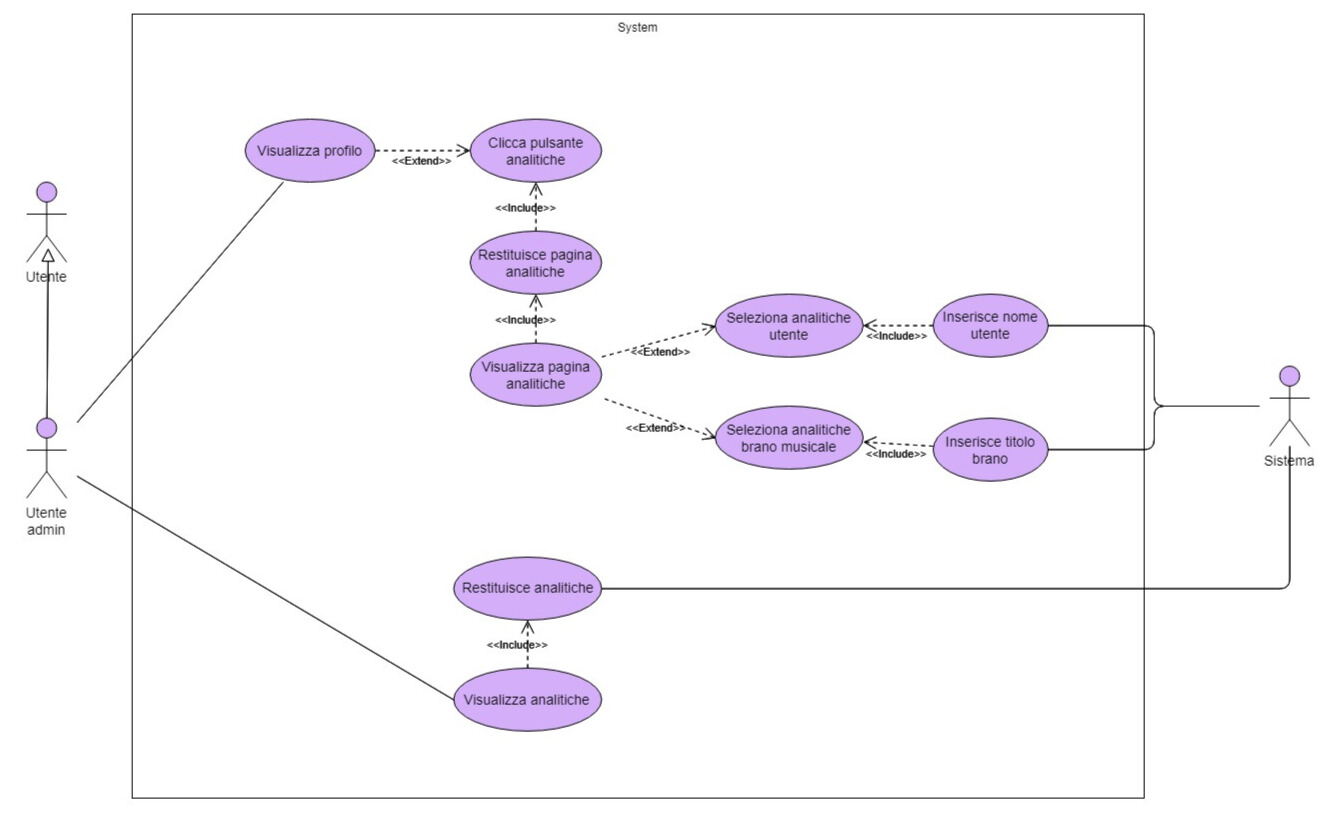
\includegraphics[width=0.9\textwidth]{Immagini/analitiche.png}
					\caption{Use Case Diagram azioni analitiche}
				\end{figure}
			\end{itemize}
			\newpage
		\subsection{Tabelle di Cockburn}
		Le tabelle di Cockburn, che devono il loro nome all'informatico Alistair Cockburn, sono un formalismo di rappresentazione di casi d'uso; la politica adotta la rappresentazione di un \textit{main} scenario nella quale uno o più attori interagiscono tra loro attraverso l'invocazione di \textit{trigger} e descrivendo gli eventi (sottoforma tabulare).\\
		Abbiamo deciso di rappresentare i seguenti Use Case:
		\begin{itemize}
			\item Aggiunta canzone ad una playlist 
			\item Azioni analitiche (ricerca e visualizzazione)
		\end{itemize}
		\newpage
		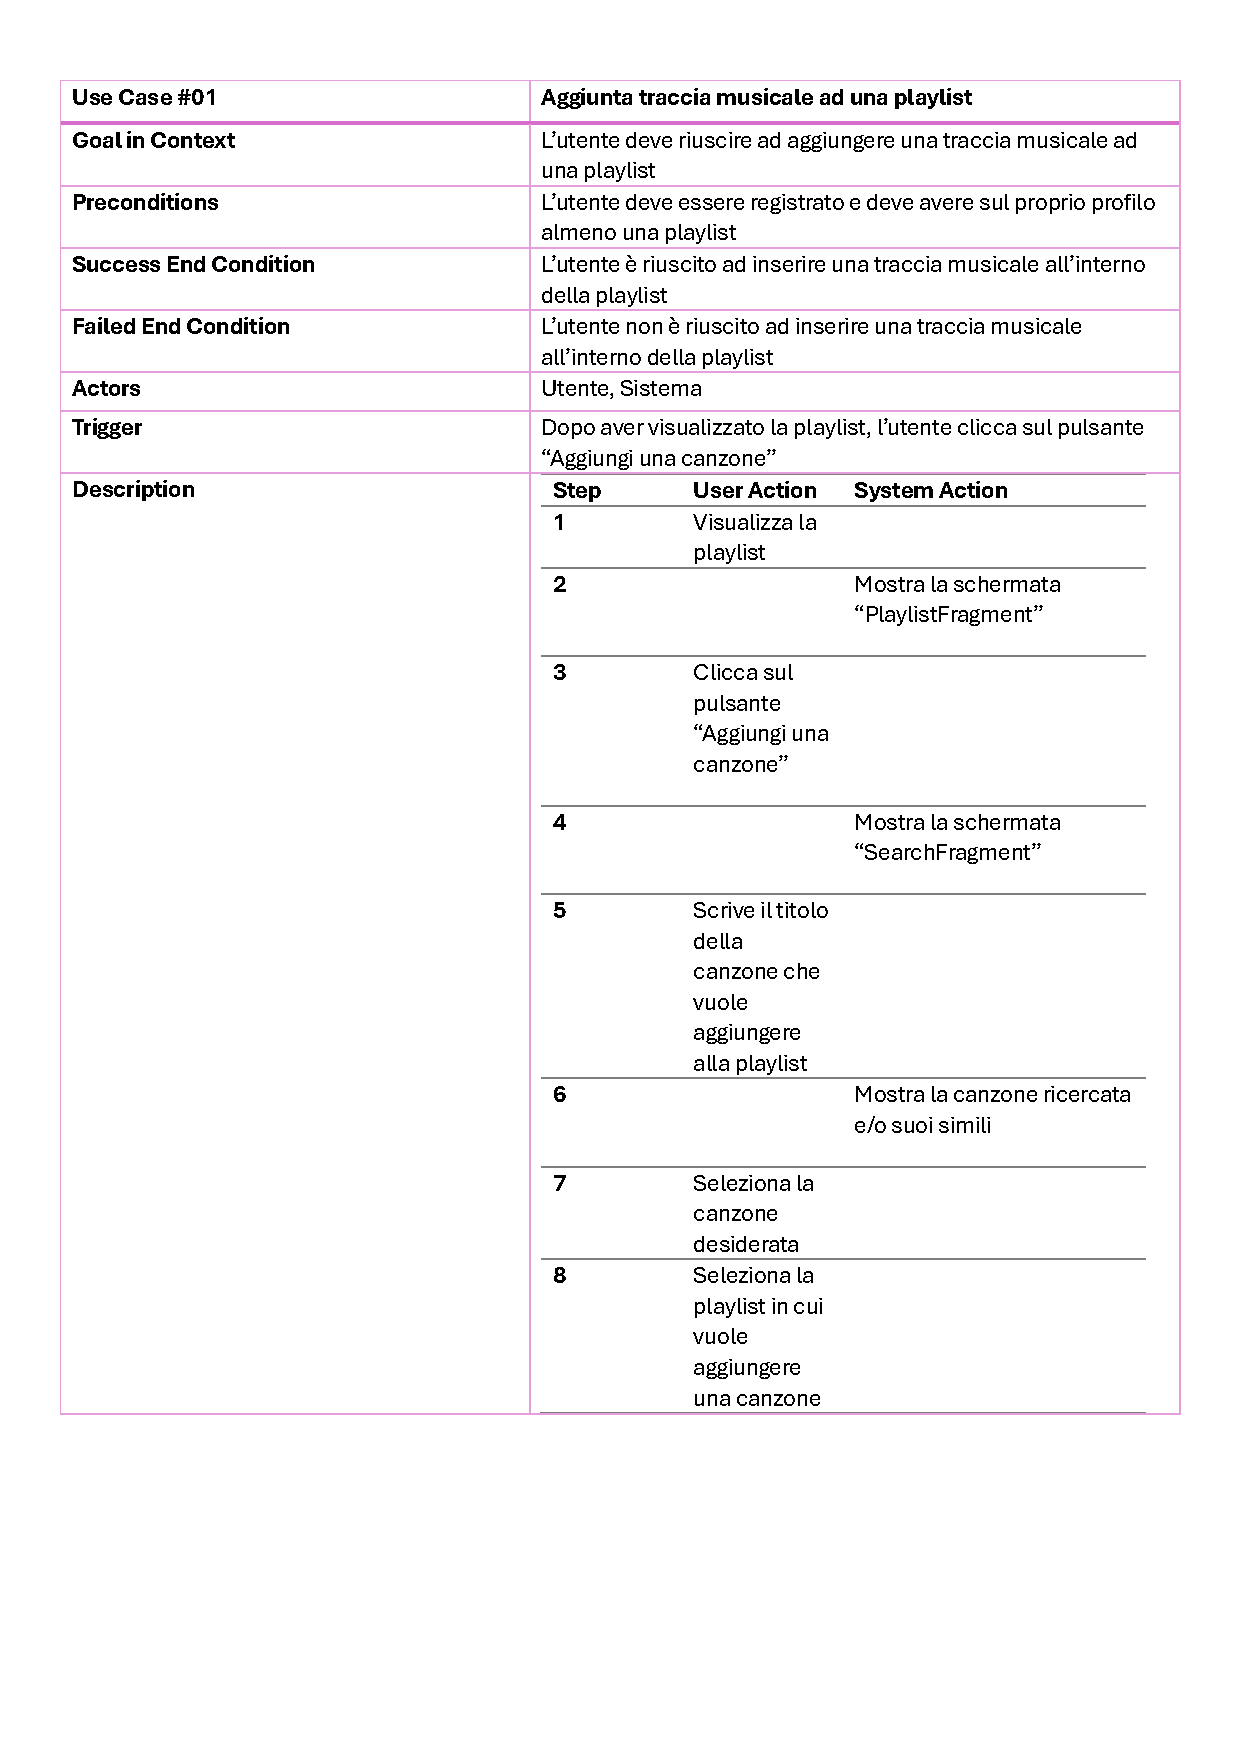
\includepdf[pages={1,2}]{Documenti/usecase.pdf}
		\newpage
		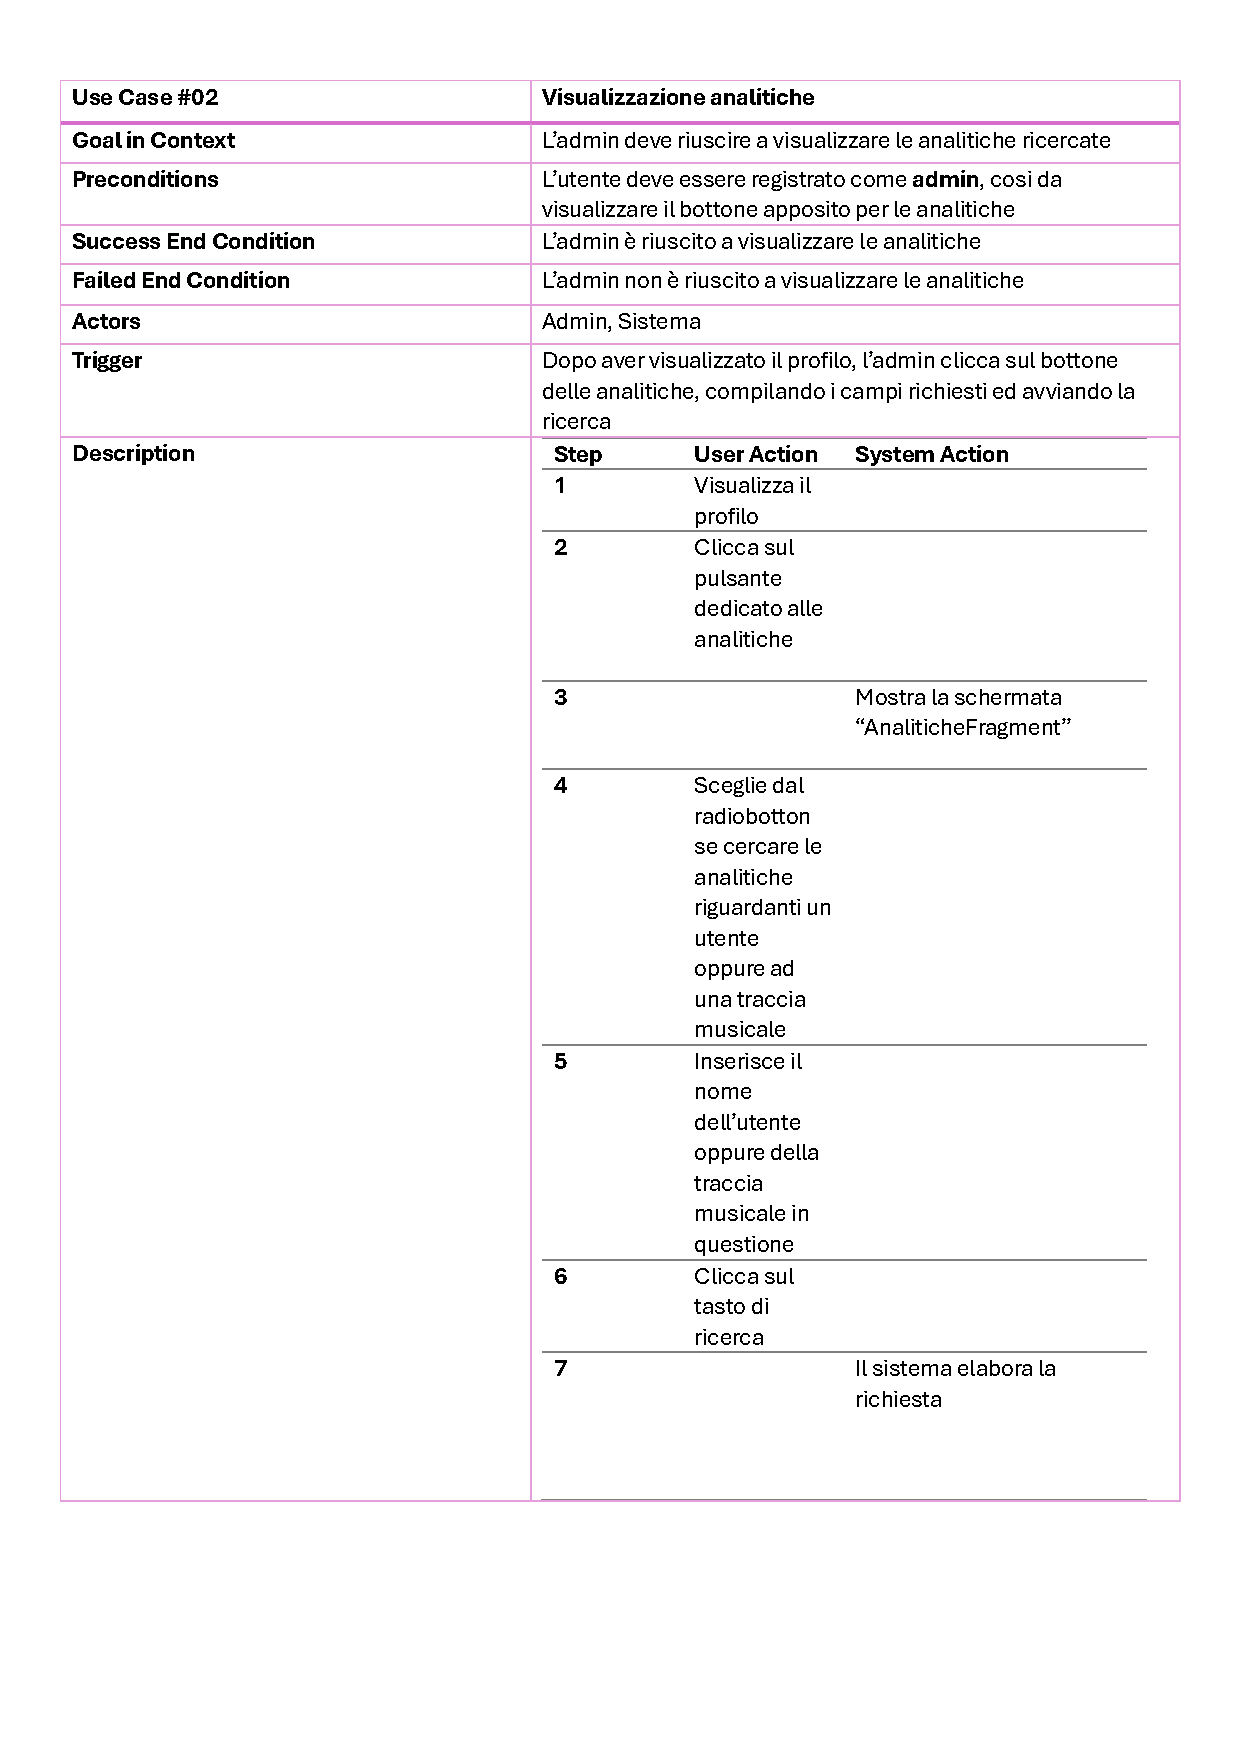
\includepdf[pages={1,2,3}]{Documenti/Cockburn2}
		\newpage
		
		\subsection{UX Design}
		Il team ha approfondito diversi studi in materia di design della \textit{user experience} e implementato quelle che sono state ritenute le scelte migliori intermini di colori, affordances e estetica per assicurare all’utente la migliore esperienza possibile sull’applicativo.\\
		In termini di realizzazione pratica della GUI, la scelta è ricaduta:
		\begin{itemize}
			\item Coerenza visiva con altre applicazioni simili per facilitarne l'uso dell'interfaccia.
			\item Impatto estetico degli elementi
			\item Adattabilità delle sue componenti con il dispositivo usato
		\end{itemize}
		Per garantire una buona esperienza utente, si concorda sull'importanza di applicare i principi della \textbf{Gestalt}, una corrente psicologia tedesca dei primi del Novecento che costruisce l'esperienza rispetto a diversi fenomeni. 
		\\Secondo la \textit{Gestalt} gli elementi simili che costituiscono un'immagine o una composizione, vengono raggruppati tra loro e poi percepiti come un unico elemento.
		\begin{figure}[H]
			\centering
			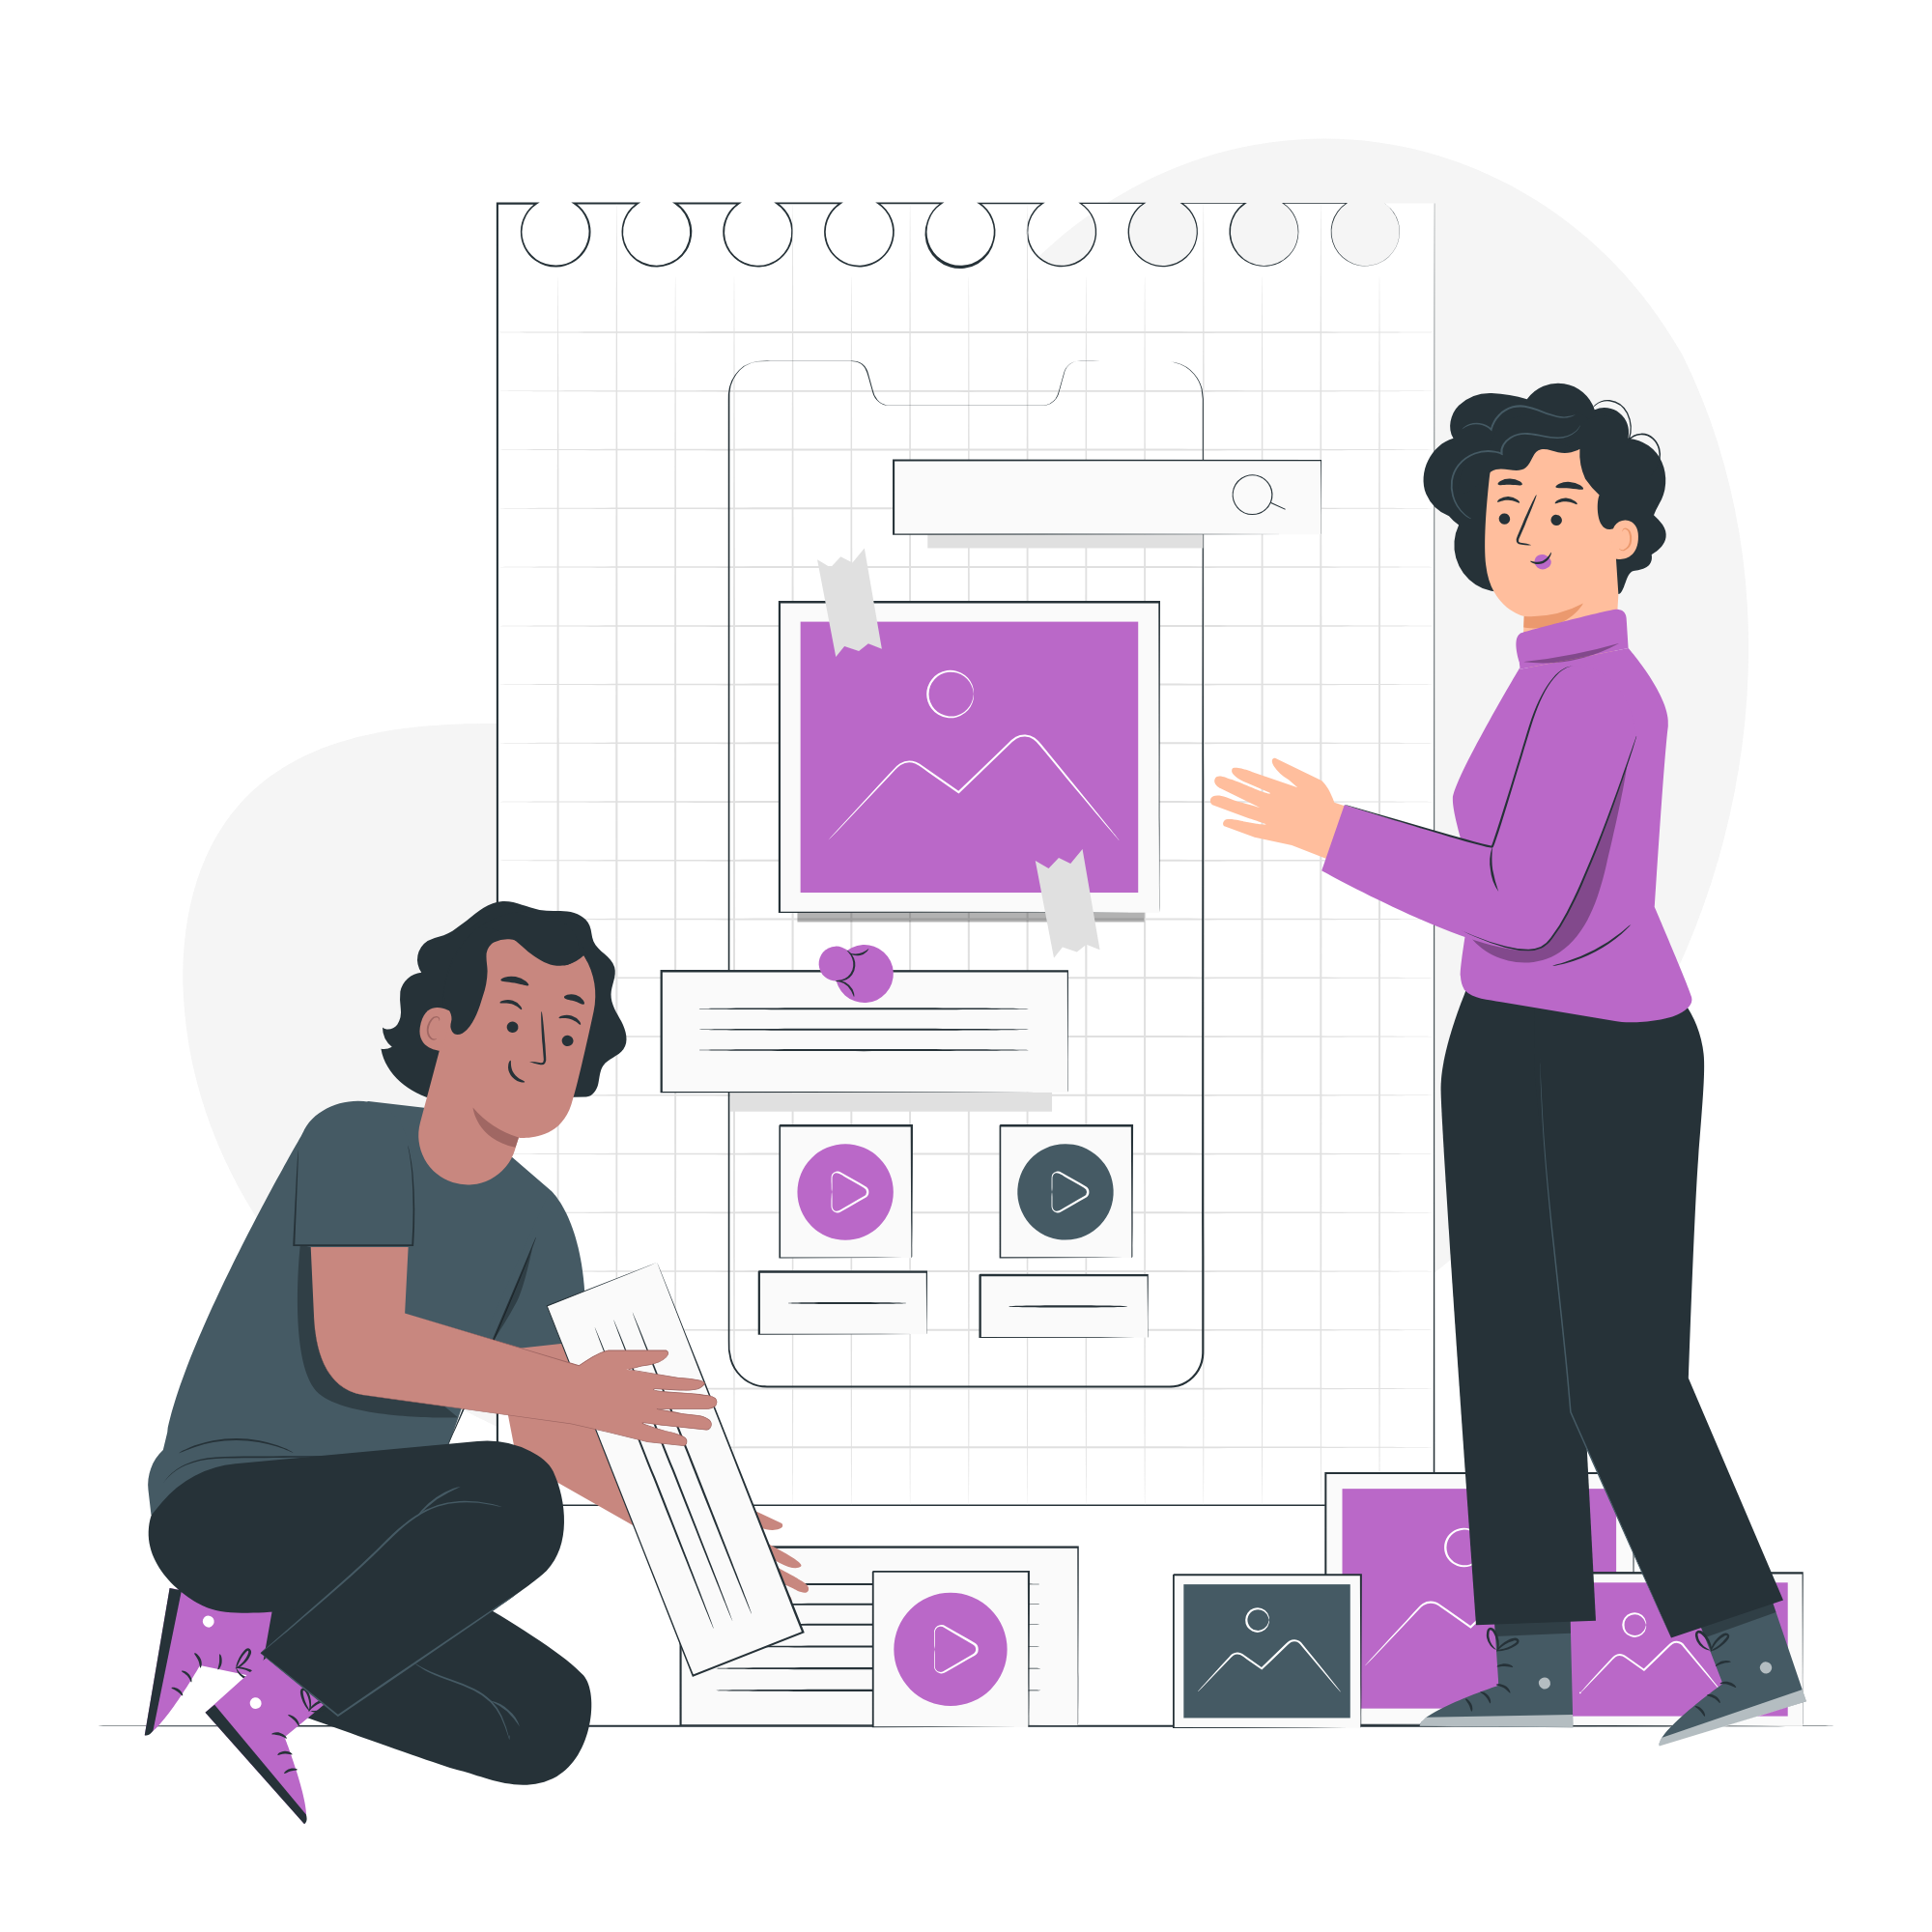
\includegraphics[width=0.6\textwidth]{Immagini/uxdesign.png}
		\end{figure}
		\textbf{Il colore e le forme} hanno, dunque, un ruolo importantissimo nella creazione di un'interfaccia utente in quanto non solo migliora l'estetica ma è un veicolo di informazioni.
		La palette colori che abbiamo deciso di utilizzare per il nostro applicativo è la seguente:
		\begin{figure}[H]
			\centering
			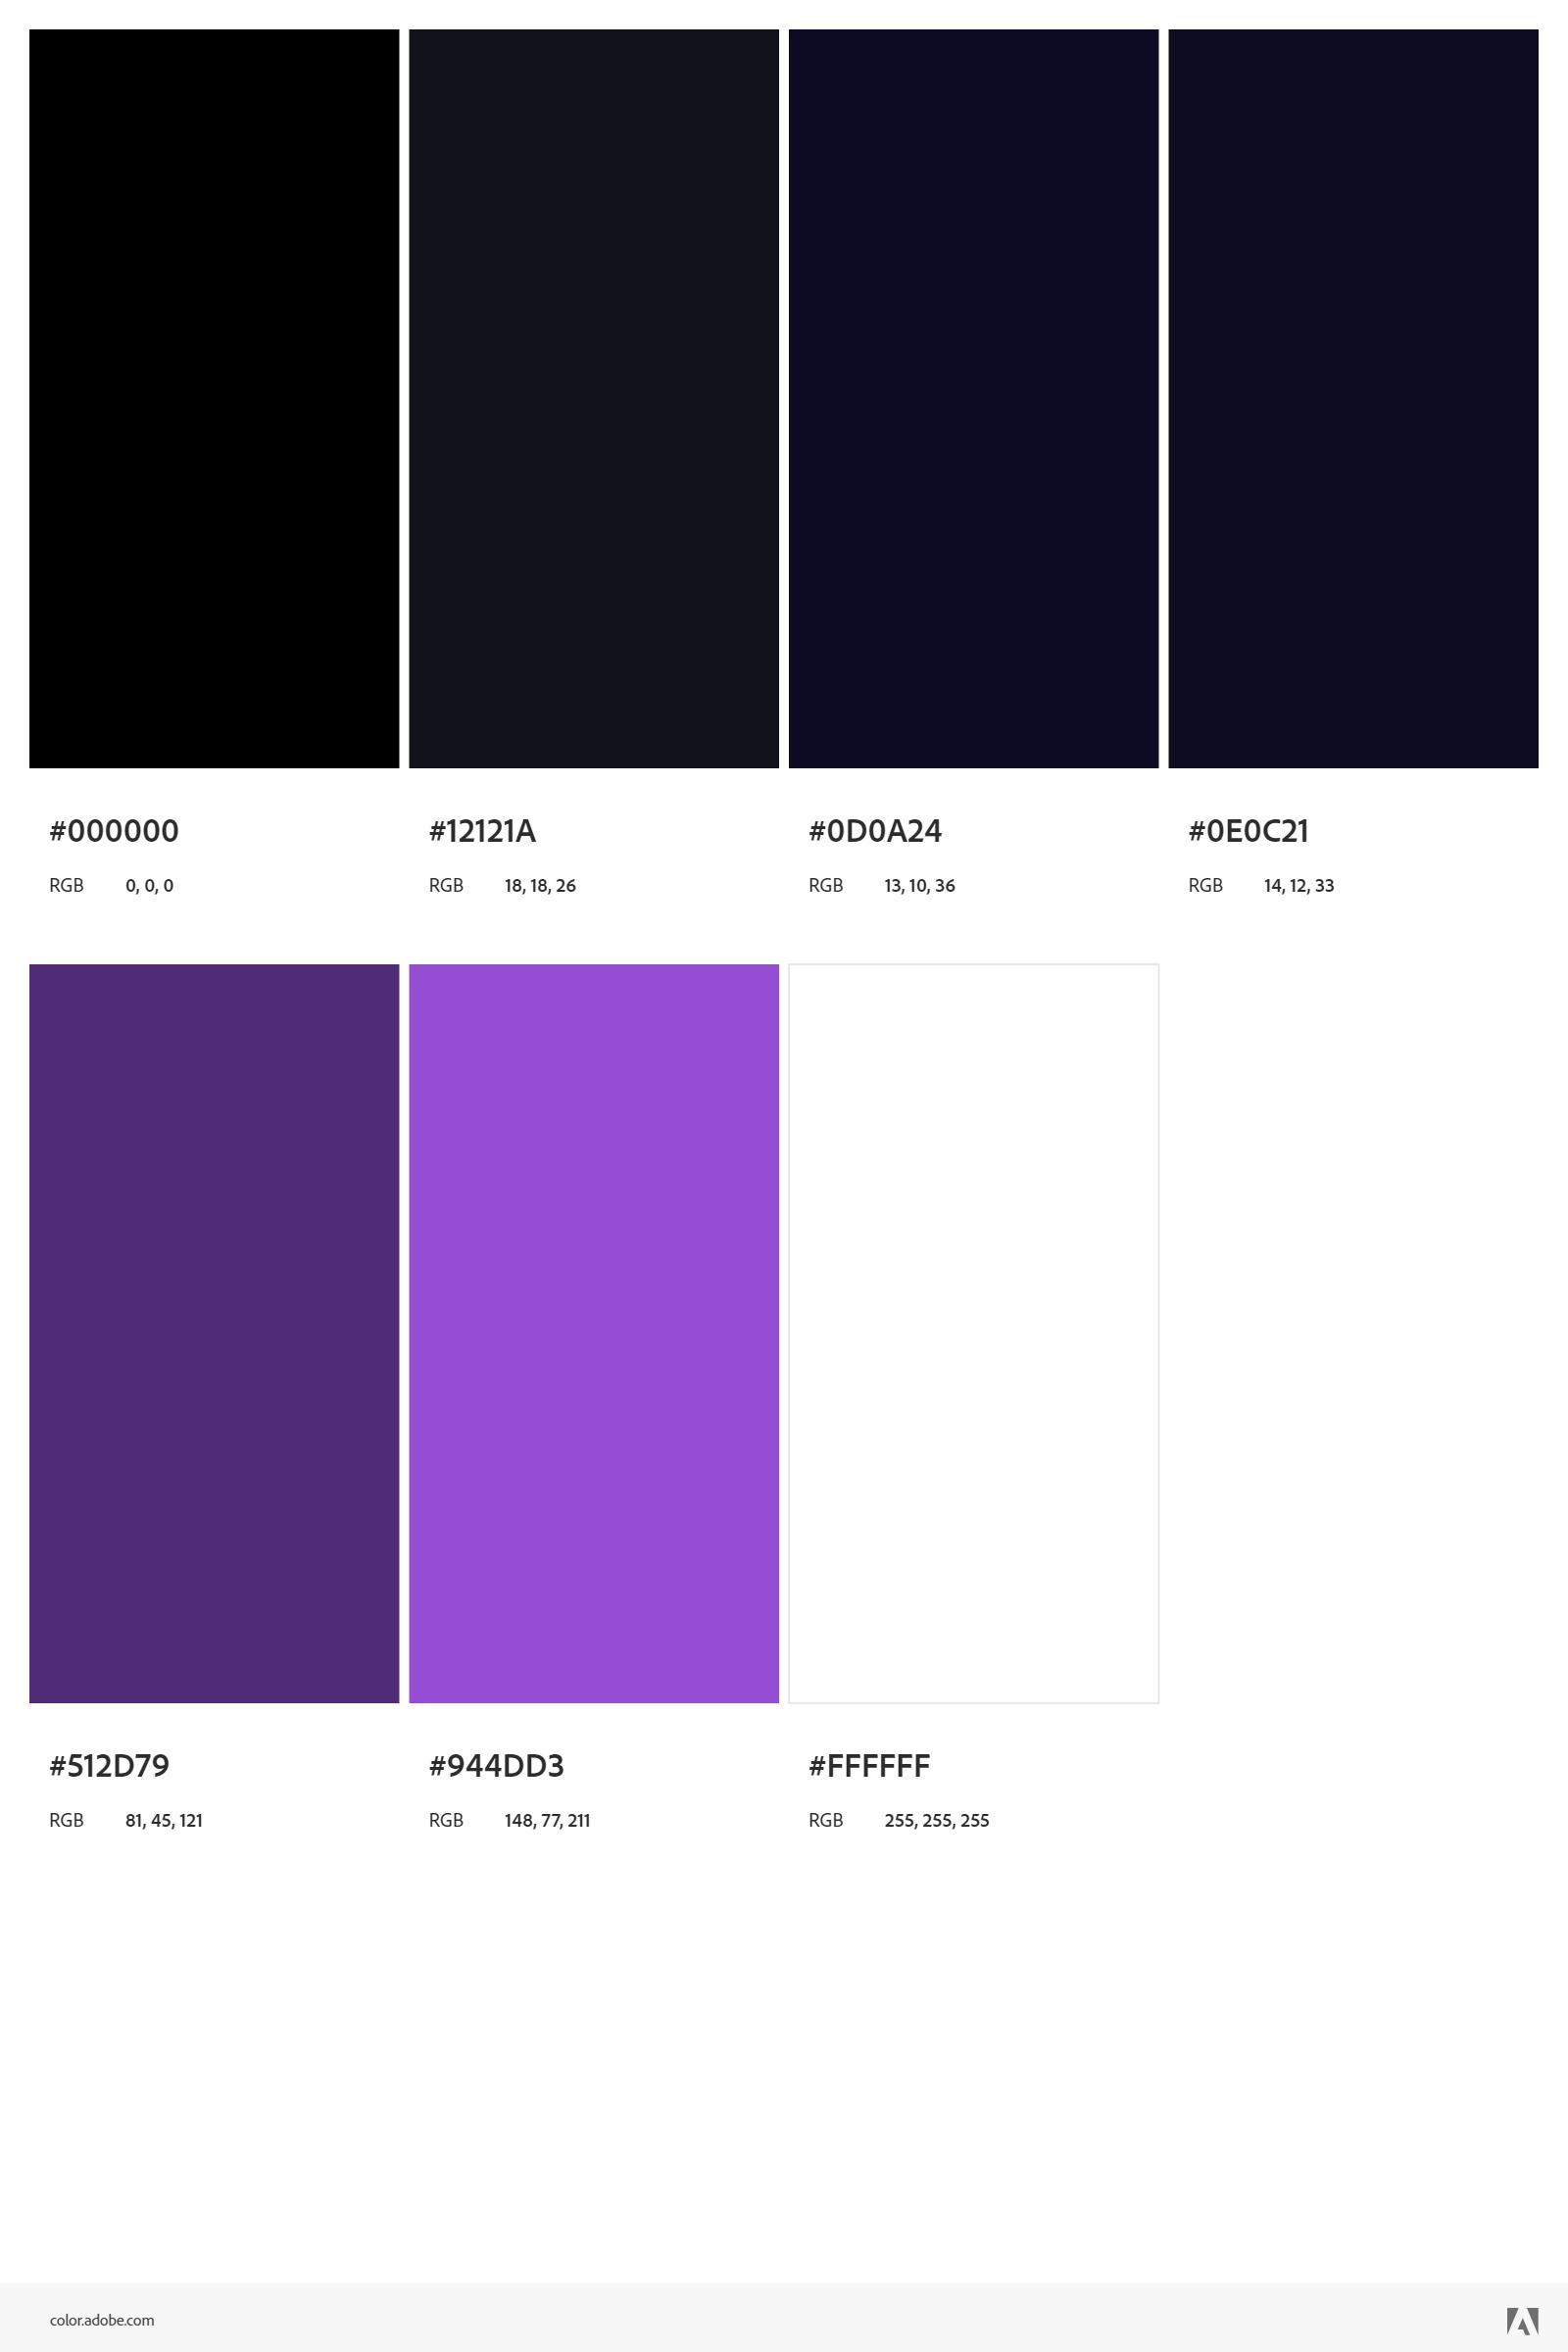
\includegraphics[width=0.6\textwidth]{Immagini/palette}
		\end{figure}
		La scelta di tale palette colori nasce dal nome stesso dell'applicativo:
		\begin{itemize}
			\item \textbf{Sound:} traduzione in inglese della parola "suono"
			\item \textbf{Lab:} diminutivo della parola inglese "Laboratory"
		\end{itemize}
		La scelta delle sfumature del color viola affiancate ai classici bianco e nero, rappresentano una forte connessione al mondo della musica ma anche al tema del laboratorio su cui verte l'applicativo.
		\begin{itemize}
			\item \textbf{Viola:} spesso associato alla creatività, all'innovazione e alla magia. Questi attributi sono fondamentali laddove si vogliano esplorare nuove idee, facendo della creatività il fulcro della composizione e dell'espressione artistica.
			\item \textbf{Nero:} colore elegante e sofisticato, che dona un aspetto raffinato e professionale. Inoltre, il nero può aiutare a mantenere il focus sugli elementi principali dell'interfaccia senza distrazioni.
			\item \textbf{Bianco:} offre un ottimo contrasto con i colori più scuri della palette, migliorando la leggibilità del testo e la visibilità degli elementi interattivi.
		\end{itemize}
		La scelta di utilizzare \textbf{forme} più tondeggianti rispetto a quelle spigolose in termini di estetica ed usabilità può influenzare significativamente l'esperienza utente.
		\begin{itemize}
			\item Le forme tondeggianti sono spesso percepite come più morbide e accoglienti rispetto a quelle spigolose.\\ Questo può creare un'atmosfera più amichevole e invitante per l'utente, contribuendo a rendere l'app più piacevole e meno intimidatoria
			\item Le curve e le linee arrotondate sono caratteristiche comuni nel design moderno e contemporaneo. \\Questi elementi possono dare all'app un aspetto più aggiornato e all'avanguardia, in linea con le tendenze attuali del design
			\item Le forme tondeggianti possono creare un senso di continuità e flusso visivo. La transizione tra gli elementi è più fluida, contribuendo a un'interfaccia più armoniosa e integrata
			\item Le forme tondeggianti possono trasmettere una sensazione di sicurezza e protezione, in quanto mancano degli angoli appuntiti che potrebbero sembrare minacciosi. \\Questo può essere particolarmente importante per utenti con esigenze di accessibilità, rendendo l'app più inclusiva
		\end{itemize}
		Fin dal prototipo iniziale, i valori citati precedentemente sono stati sempre rispettati.\\
		Bisogna specificare, però, che in fase di sviluppo molte scelte stilistiche sono state modificate per garantire una funzionalità maggiore dell'applicativo.\\
		Per una visione completa dei mockup dell'applicazione, si consiglia di cliccare il seguente link: \href{https://www.figma.com/design/Ydobs9LpJIG0QtayPxFLHQ/SoundLab?node-id=0-1&t=WTyvVfdrgmC9HQYu-1}{Figma - SoundLab}
		\hspace{0.1\textwidth}
		\begin{center}
			\begin{figure}[htbp]
				\centering
				\begin{minipage}[t]{0.2\textwidth}
					\centering
					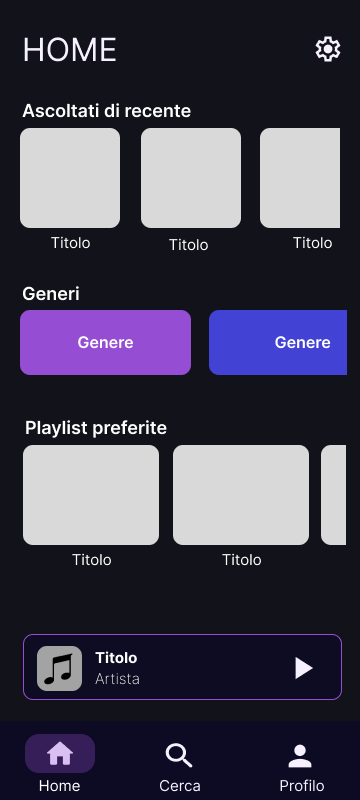
\includegraphics[width=\textwidth]{Immagini/home_page}
					\caption{Prototipo iniziale della schermata di home}
					\label{fig:home_page}
				\end{minipage}%
				\hspace{0.1\textwidth}
				\begin{minipage}[t]{0.2\textwidth}
					\centering
					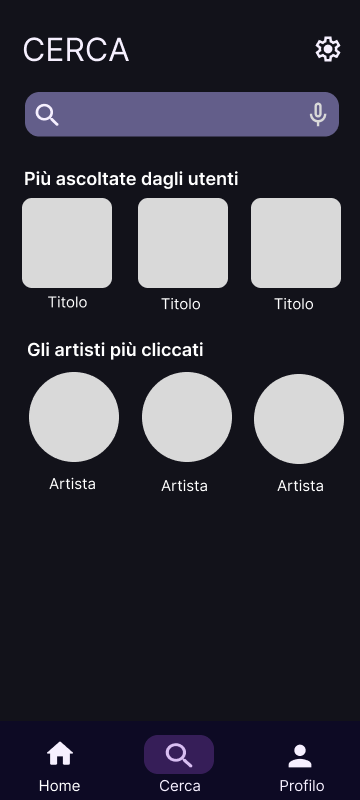
\includegraphics[width=\textwidth]{Immagini/search_page}
					\caption{Prototipo iniziale della pagina di ricerca}
					\label{fig:search_page}
				\end{minipage}
			\end{figure}
		\end{center}
		\newpage
		
			\subsubsection{Mockup}
			Il mockup è una rappresentazione visiva del prodotto o dell’idea, utilizzata per valutarne l’aspetto e l’organizzazione. È un modello statico e illustra l’aspetto e il funzionamento previsto di un prodotto, per esempio.\\
			Esso comprende elementi, come per esempio l’aspetto grafico (i loghi, le immagini, i colori, le visualizzazioni della navigazione, ecc.), che saranno utilizzati nel design finale e nell’esperienza dell’utente.
			In sostanza, un mockup serve a mostrare agli stakeholder e agli utenti come potrebbe essere il progetto o il prodotto finito, offrendone un’idea visiva chiara e dettagliata del design e delle funzionalità.\\
			I mockup sono stati fatti utilizzando come tool-case \textbf{Figma}. Di seguito, una prima versione del \textit{mockup}\footnote{L'applicativo finale rispecchia in pieno i mockup iniziali. Tuttavia, bisogna specificare che in fase di sviluppo alcune scelte stilistiche sono state modificate per favorire la user experience}.
			\begin{figure}[htbp]
				\centering
				\begin{minipage}{0.18\textwidth}
					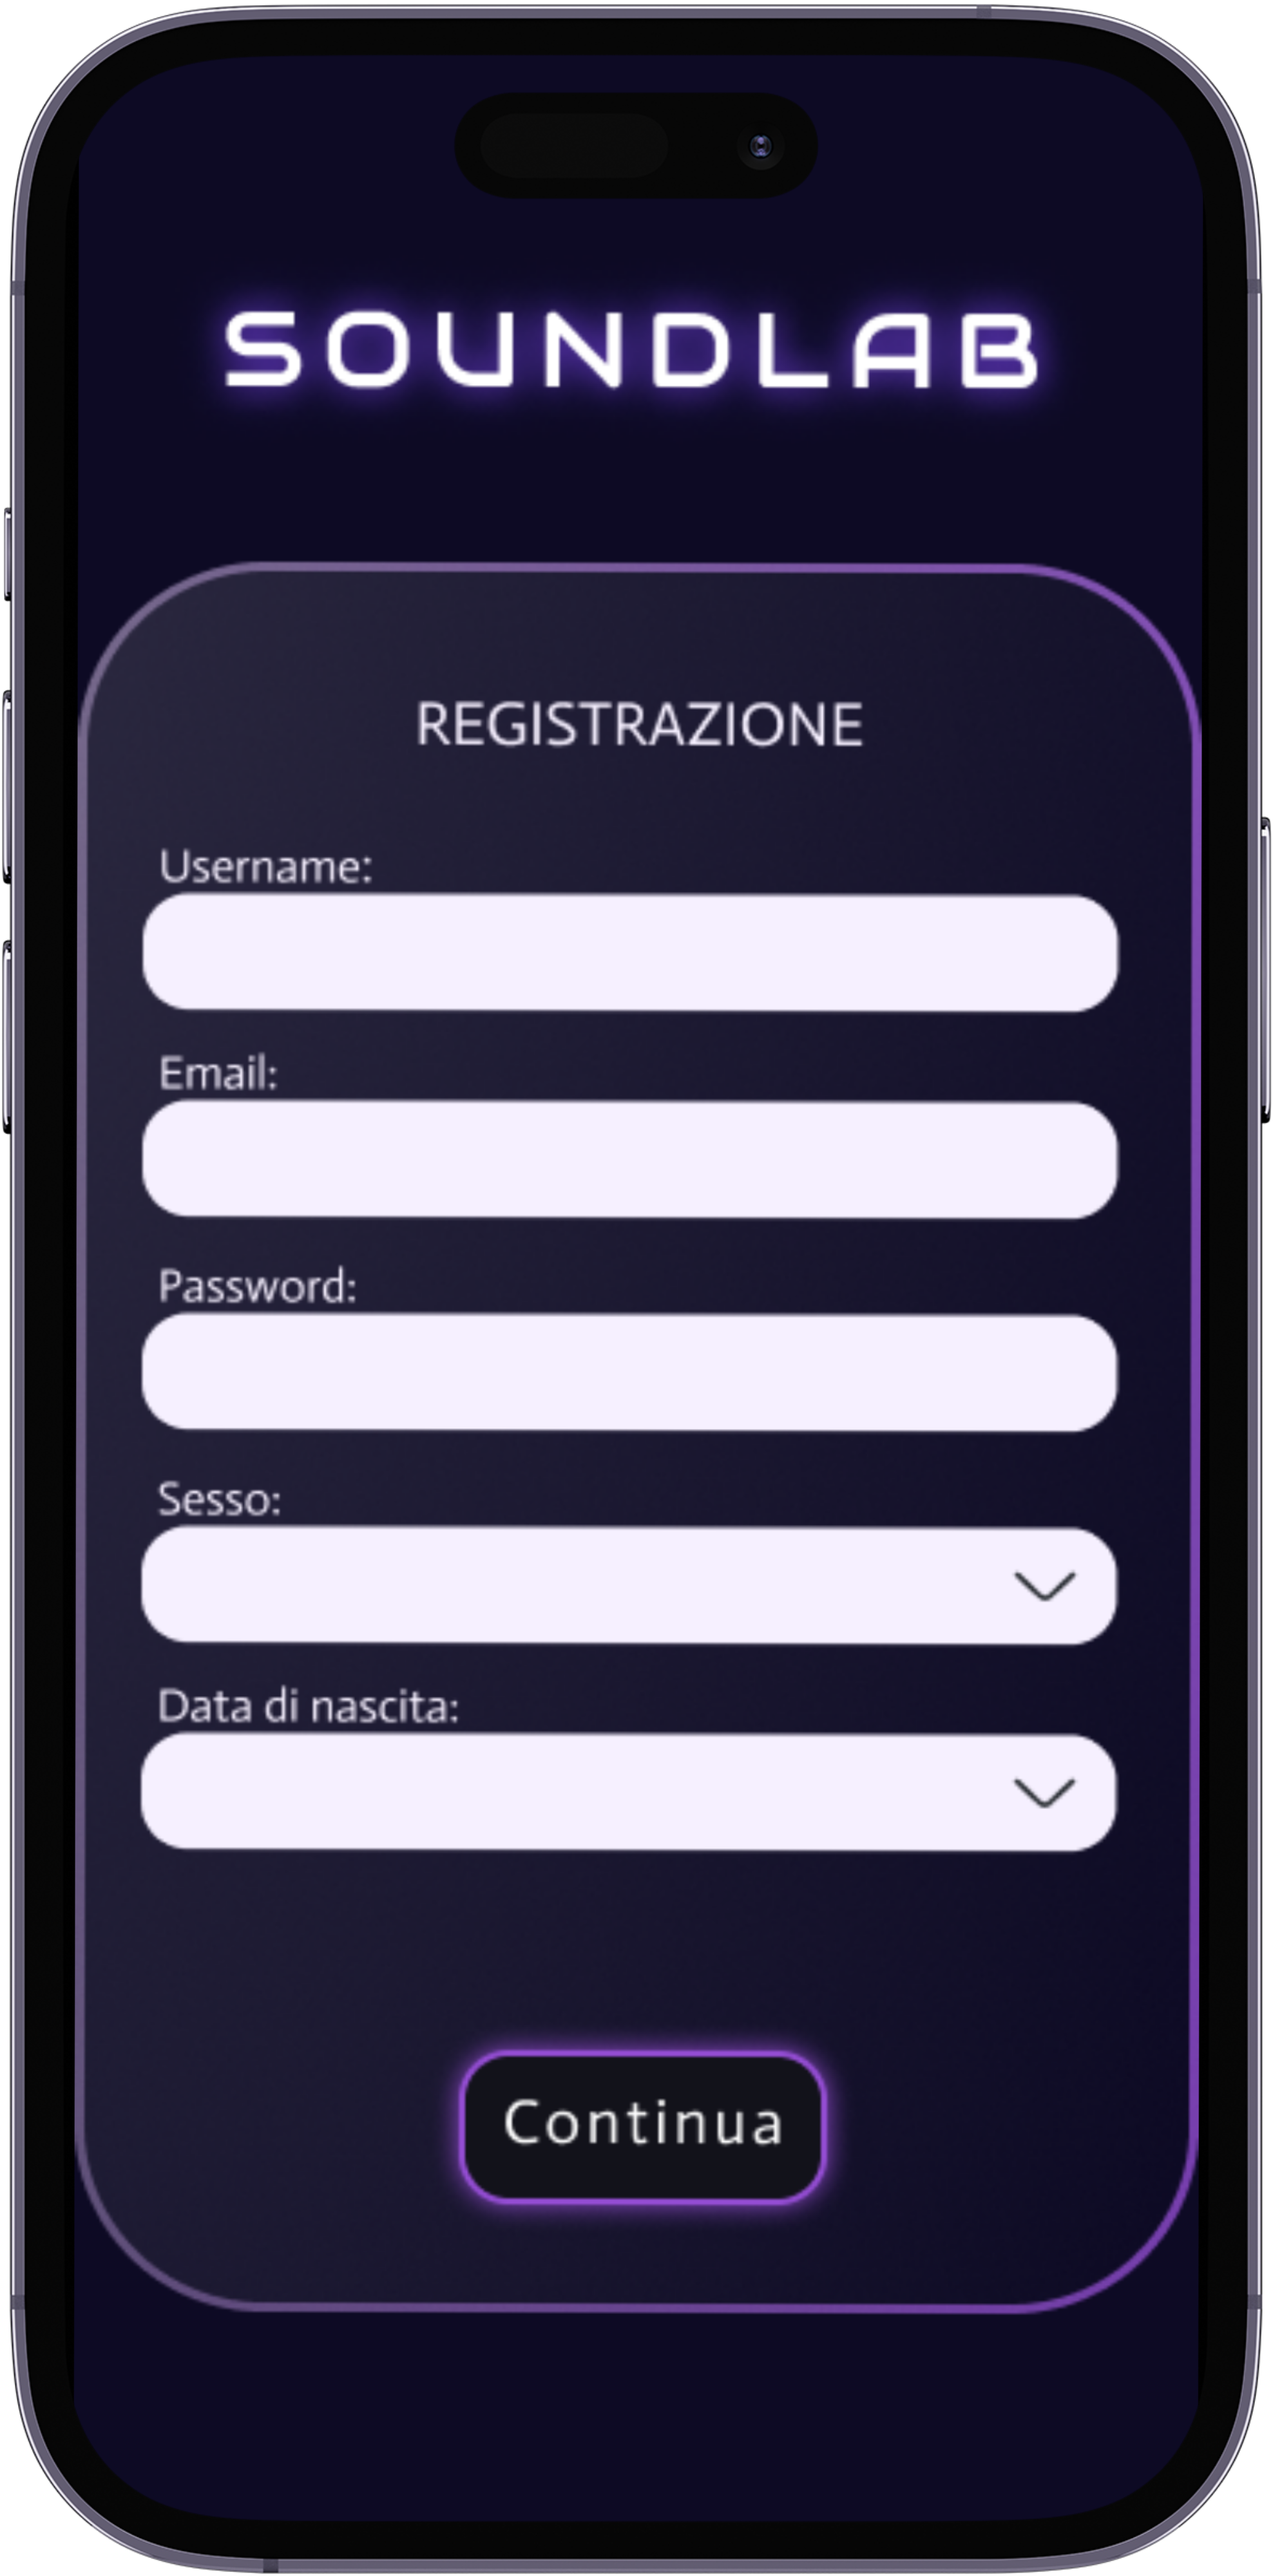
\includegraphics[width=\textwidth]{Immagini/foto1}
				\end{minipage}
				\hfill
				\begin{minipage}{0.18\textwidth}
					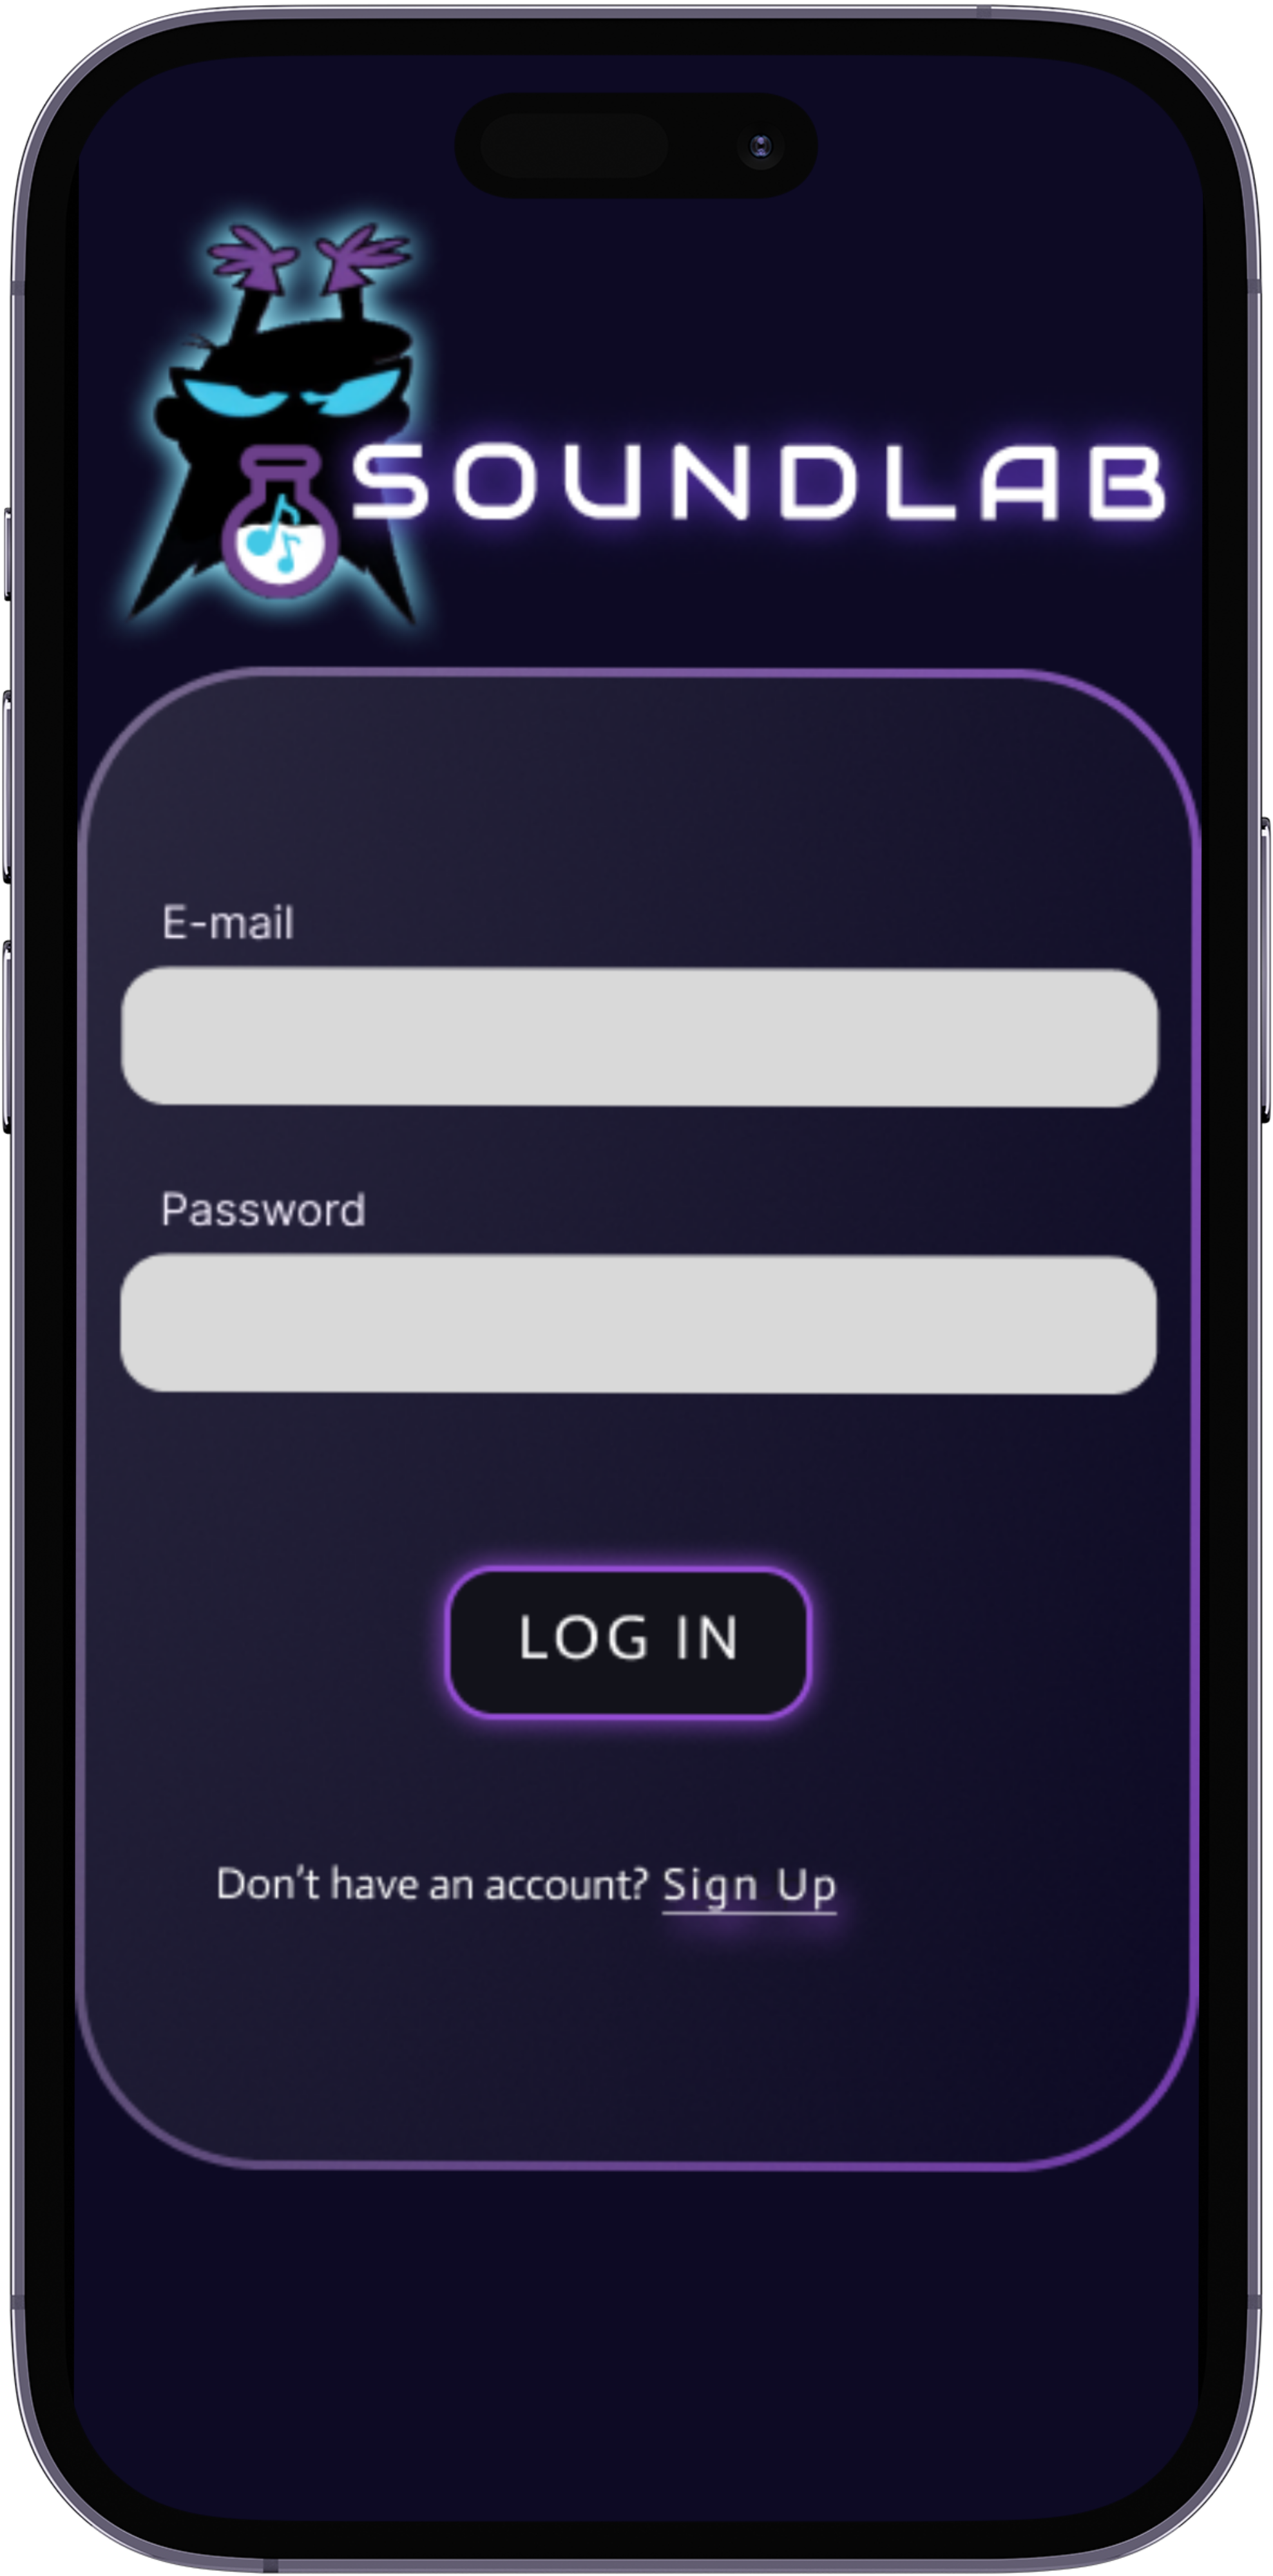
\includegraphics[width=\textwidth]{Immagini/foto2}
				\end{minipage}
				\hfill
				\begin{minipage}{0.18\textwidth}
					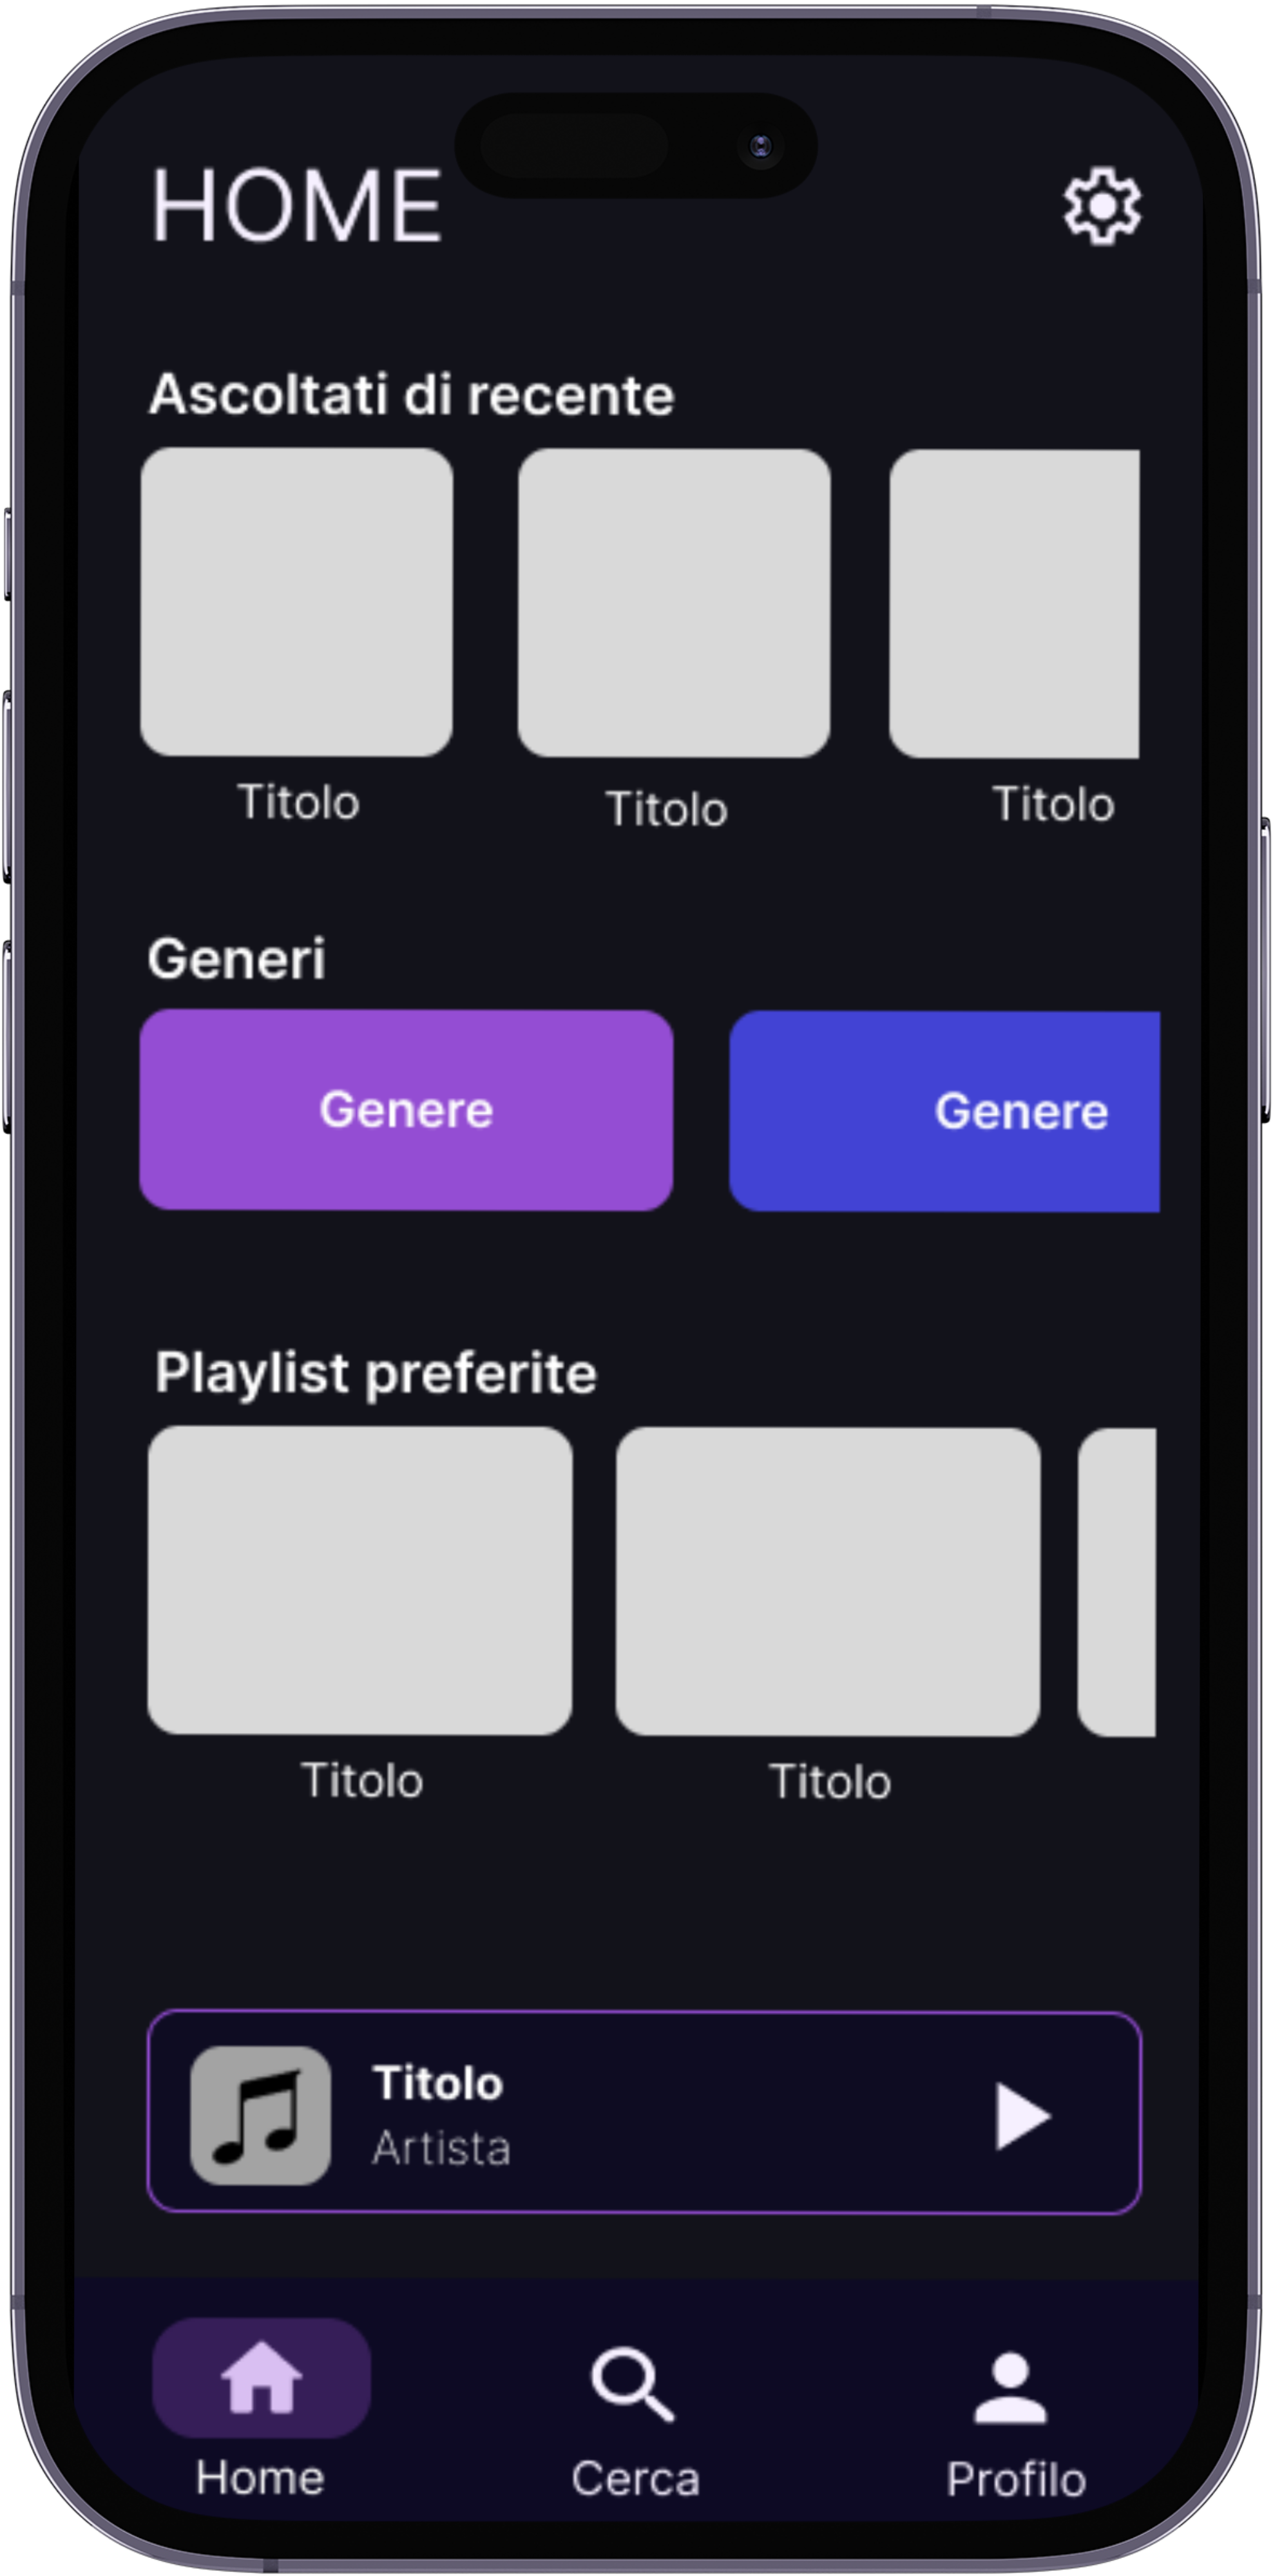
\includegraphics[width=\textwidth]{Immagini/foto3}
				\end{minipage}
				\hfill
				\begin{minipage}{0.18\textwidth}
					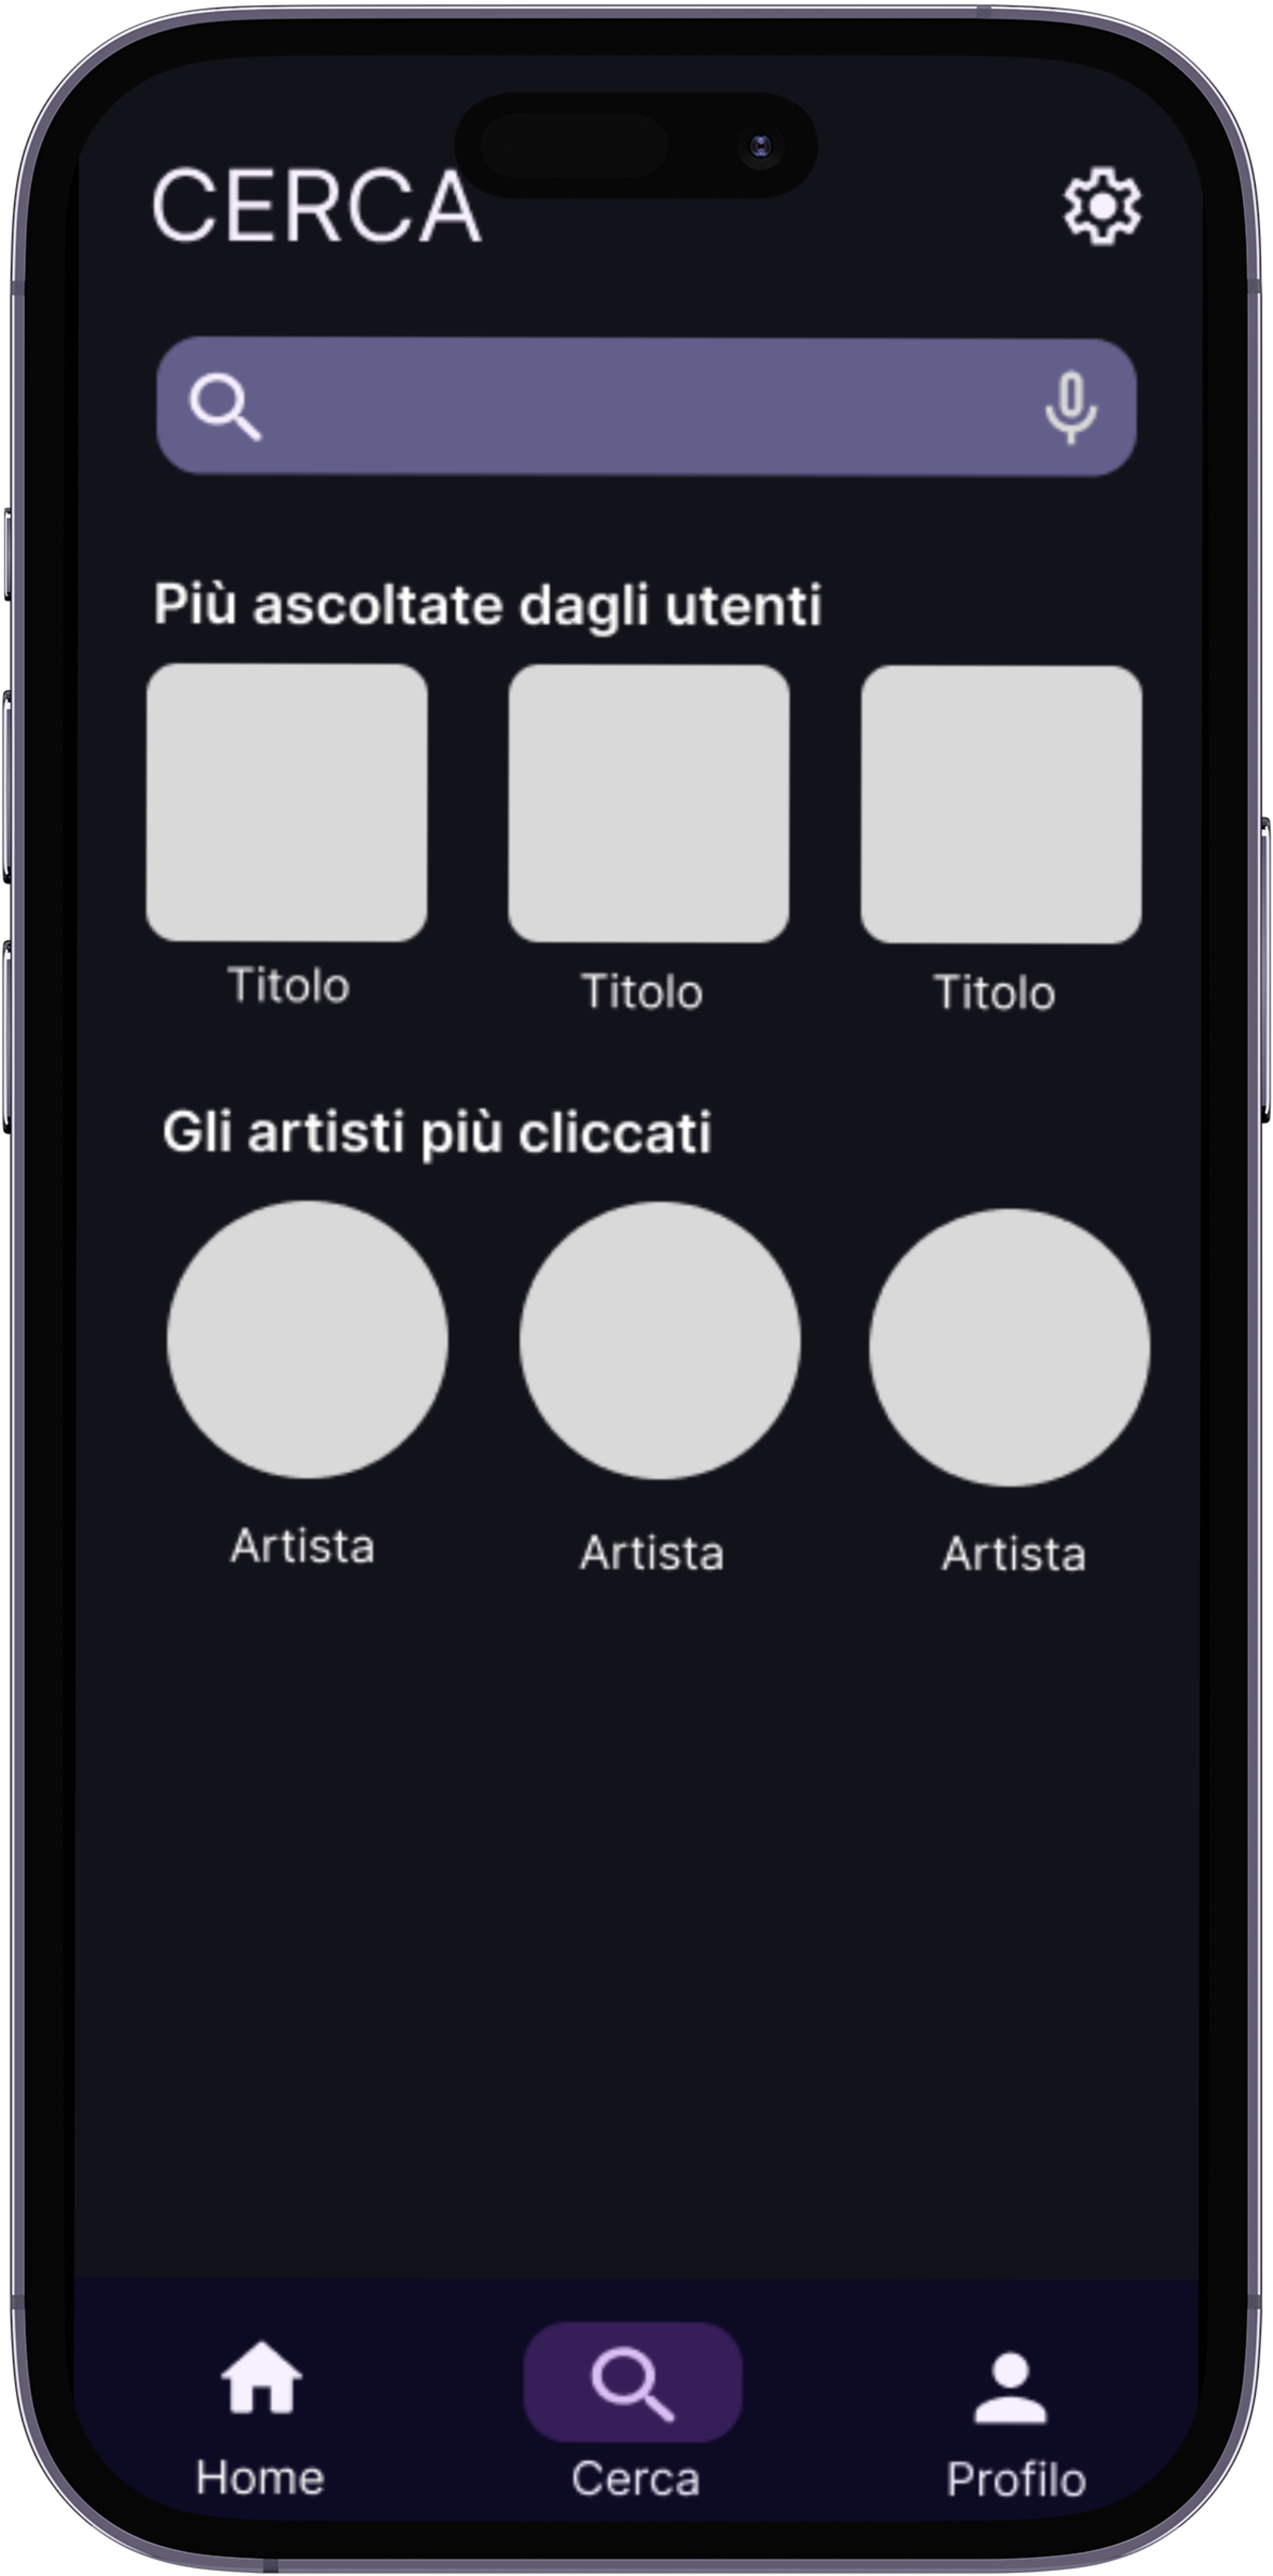
\includegraphics[width=\textwidth]{Immagini/foto4}
				\end{minipage}
				\hfill
				\begin{minipage}{0.18\textwidth}
					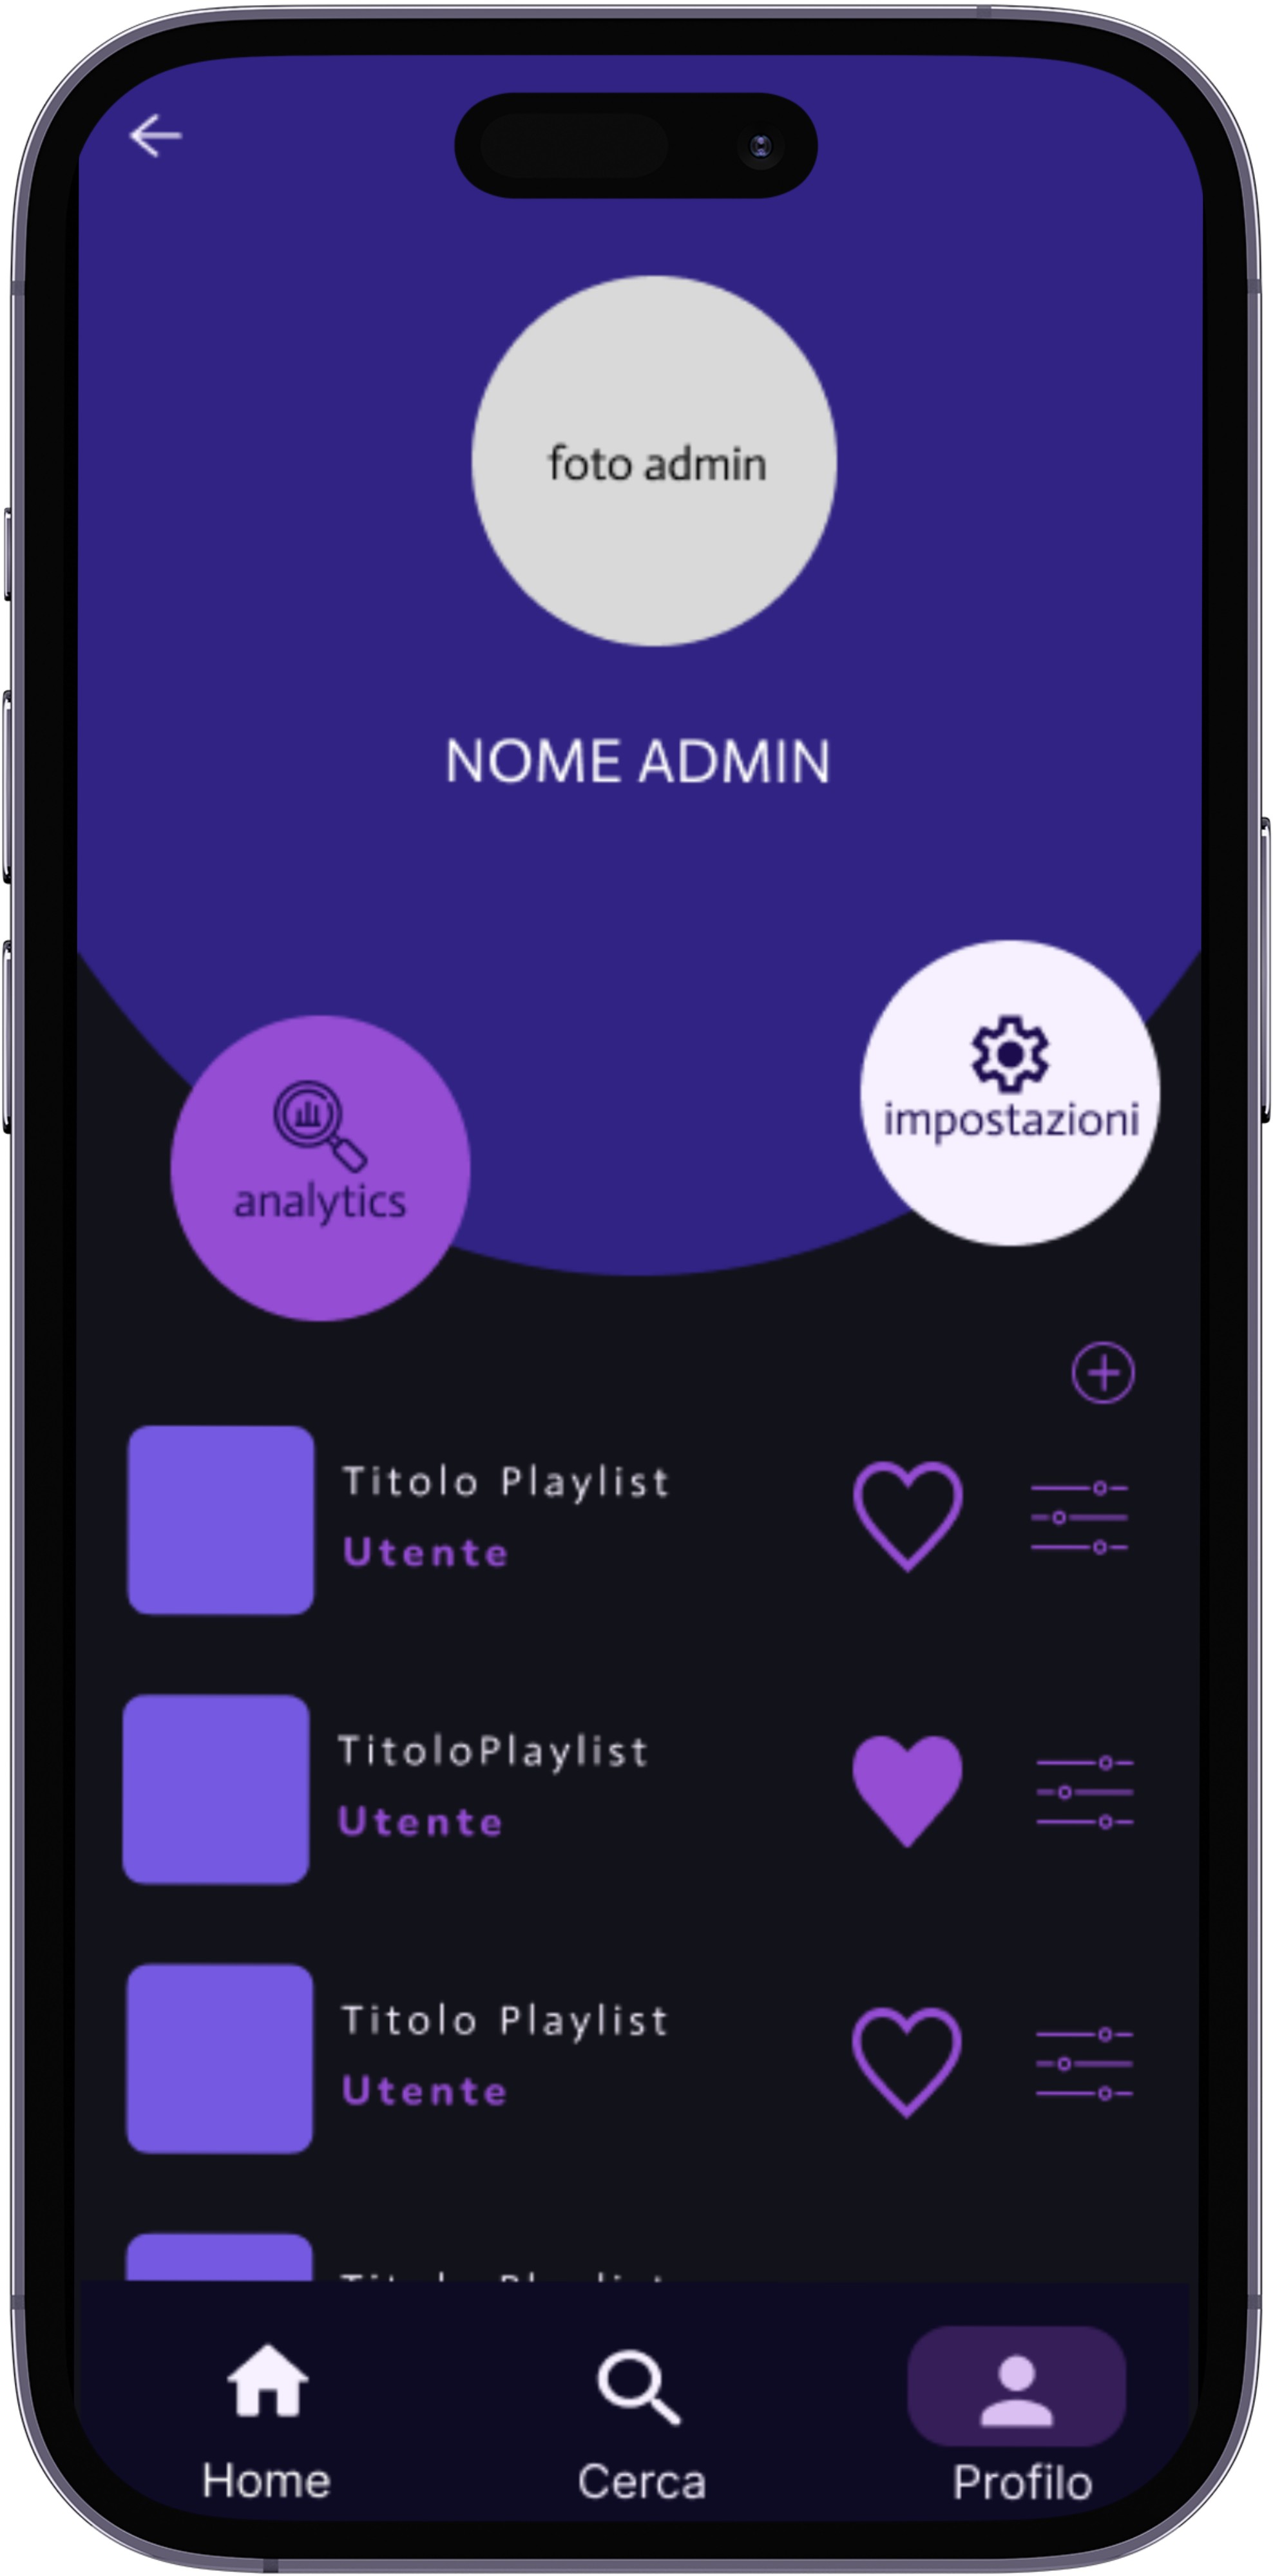
\includegraphics[width=\textwidth]{Immagini/foto6}
				\end{minipage}
				\hfill
				\begin{minipage}{0.18\textwidth}
					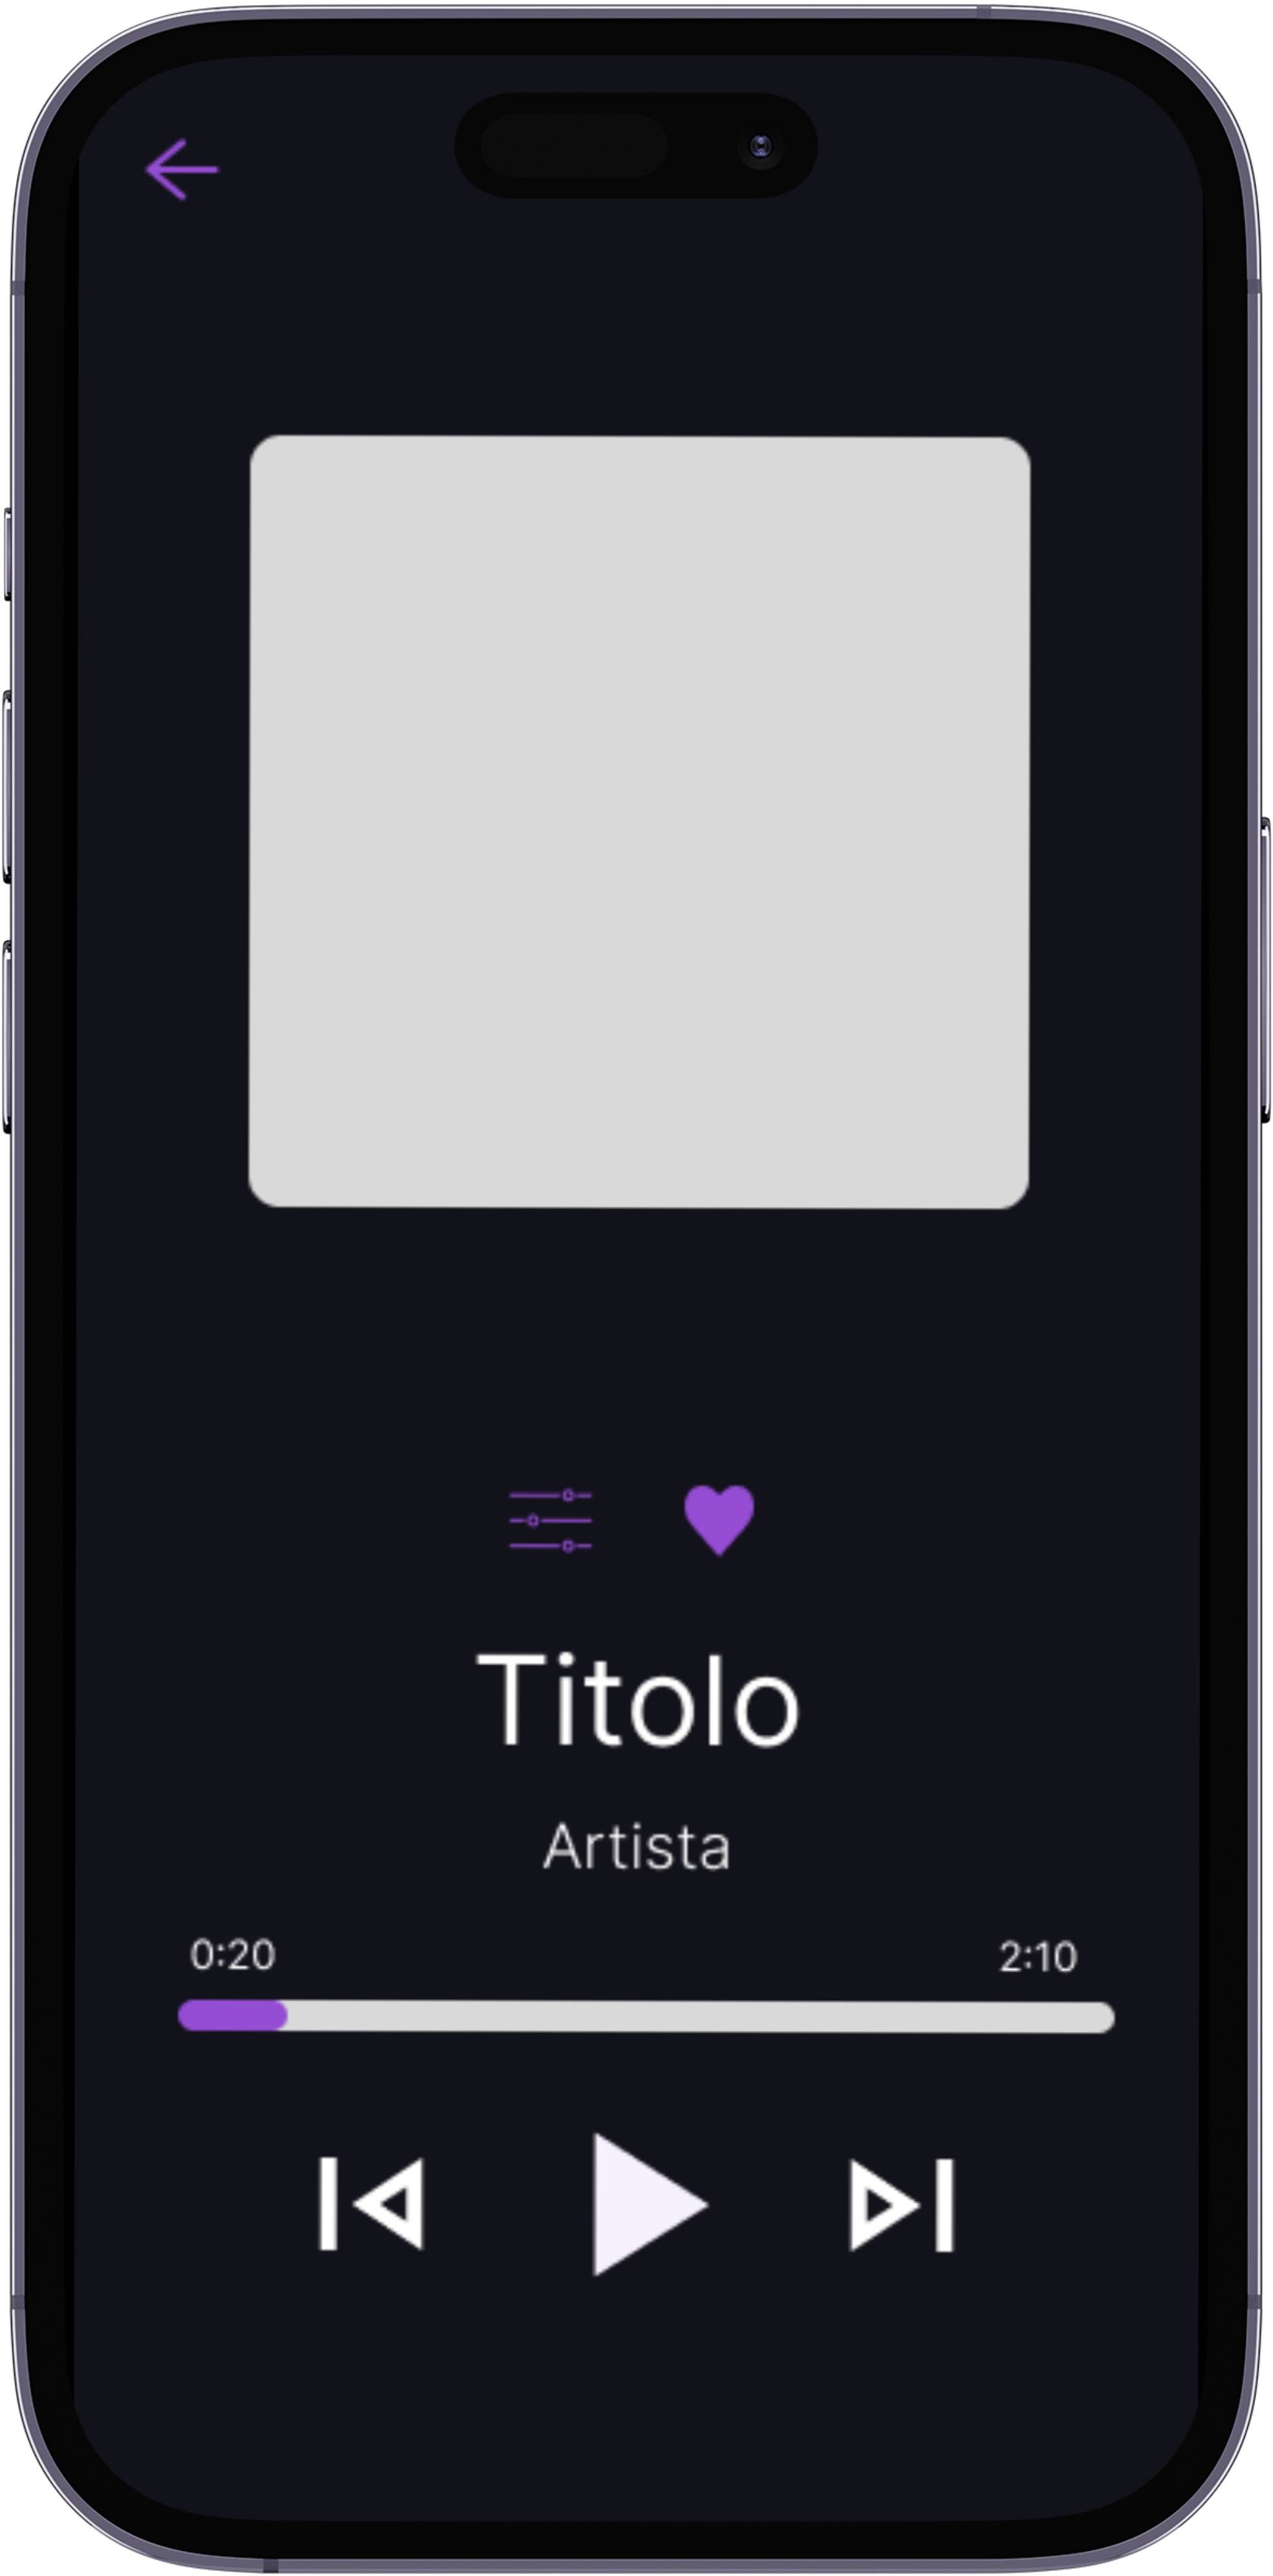
\includegraphics[width=\textwidth]{Immagini/foto7}
				\end{minipage}
			\end{figure}
			\newpage
		Verranno mostrati, di seguito, i\textit{ mockup finali} di due metodi scelti ovvero: \textbf{visualizzazione analitiche} e \textbf{aggiunta traccia musicale ad una playlist}.
			\subsubsection{Mockup Visualizzazione analitiche}
			\textit{NOTA: è stato ritenuto opportuno riportare anche un caso d'errore.}
			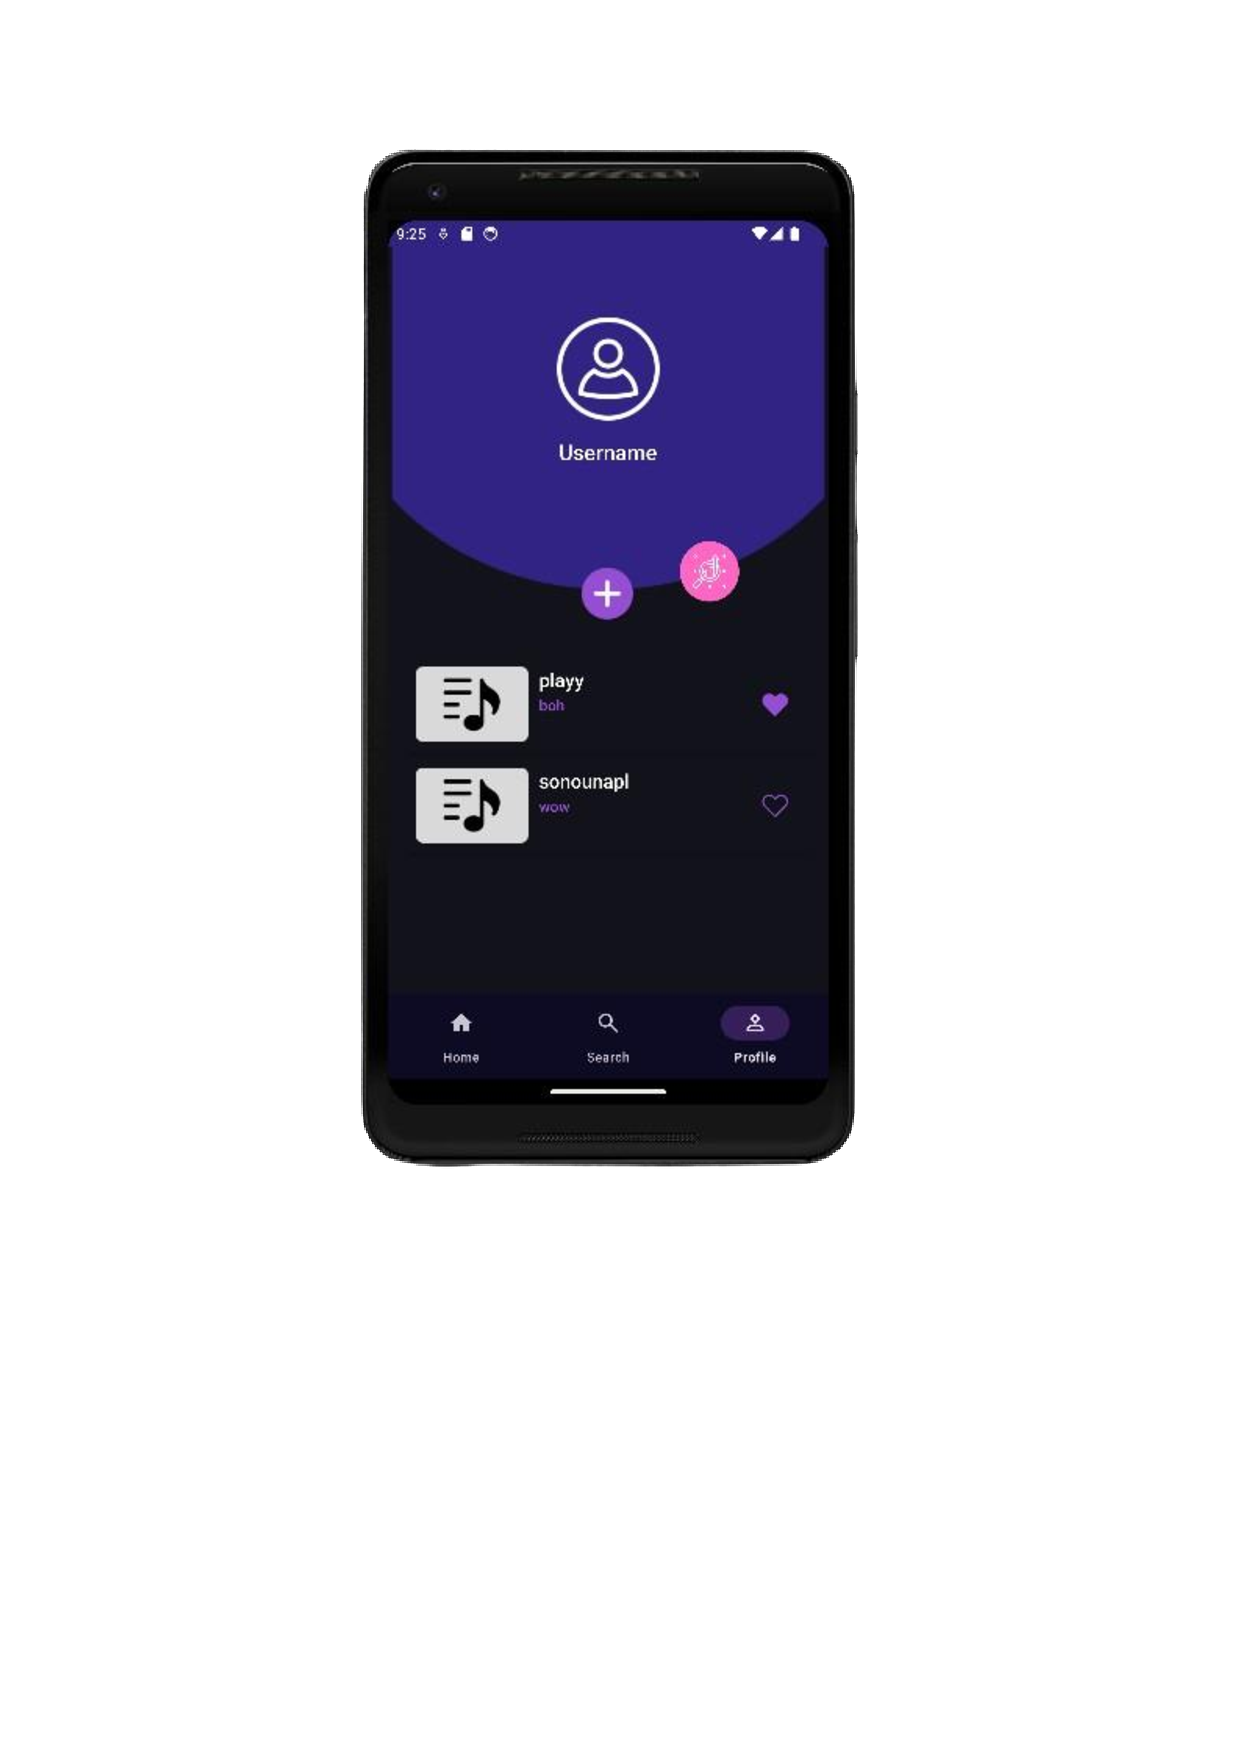
\includepdf[pages={1,2,3,4,5,6,7}]{Documenti/mockupanalitiche}
			
			\subsubsection{Mockup Aggiunta traccia musicale ad una playlist}
			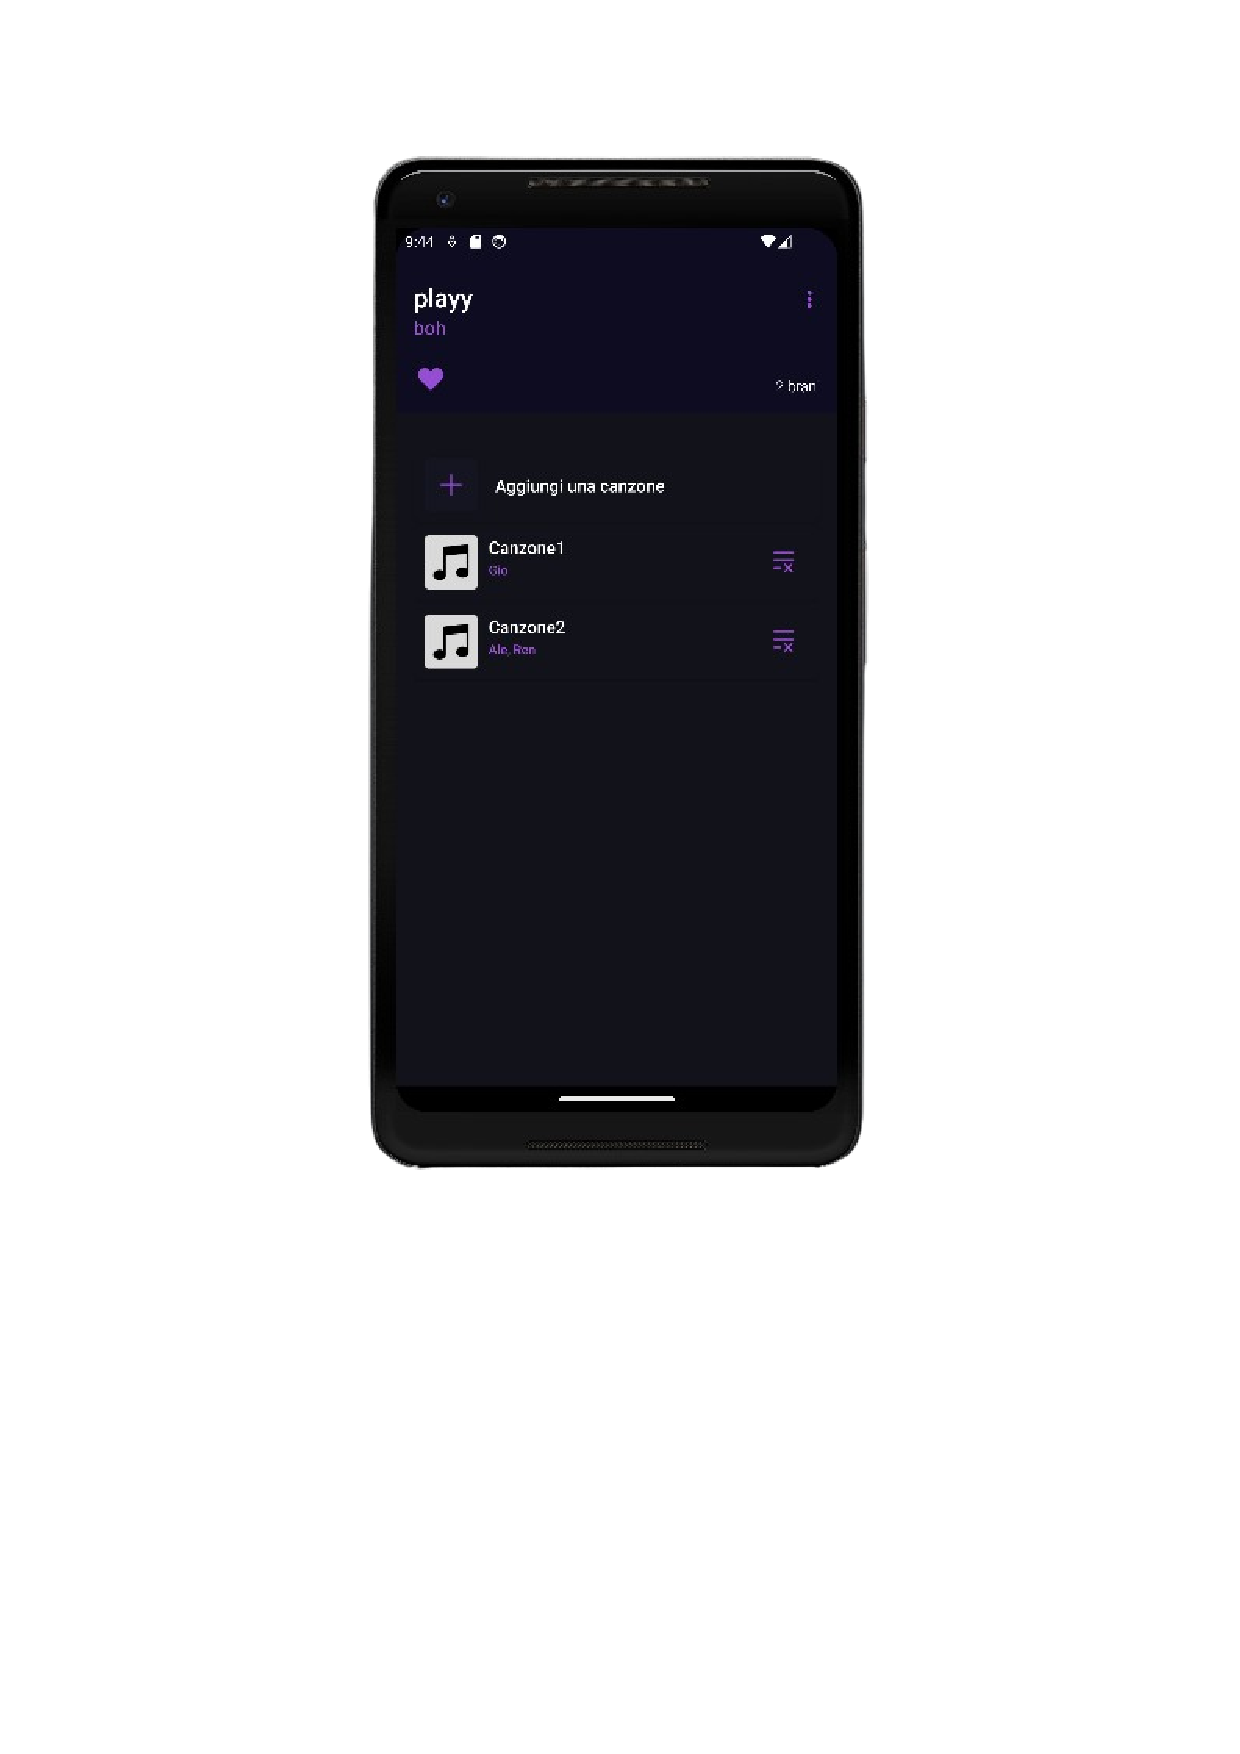
\includepdf[pages={1,2,3,4}]{Documenti/mockupadd}
		\subsection{Presentazione dell'idea progettuale}
		\textbf{\textit{\textcolor{dark_purple}{Soundlab}}} nasce dall'esigenza di creare una piattaforma di streaming musicale che offra condizioni più vantaggiose per gli artisti, garantendo una remunerazione più equa e trasparente. Inoltre, si propone di migliorare significativamente l'esperienza dell'utente attraverso un'interfaccia più intuitiva e funzionalità innovative che permettano una maggiore personalizzazione dei contenuti.\\
		\textbf{\textit{\textcolor{dark_purple}{Soundlab}}} mira anche a differenziarsi con un catalogo musicale unico, promuovendo così una maggiore diversità musicale. Infine, una priorità fondamentale è garantire una maggiore tutela della privacy e sicurezza dei dati degli utenti, rispondendo alle crescenti preoccupazioni riguardo alla gestione delle informazioni personali.
		
			\subsubsection{Perchè abbiamo deciso di lavorare con la musica?}
			Al giorno d'oggi, lavorare con la musica o attraverso piattaforme ad essa dedicate offre numerosi vantaggi.\\ Innanzitutto, la \textbf{crescente diffusione della tecnologia} e \textbf{l'accesso a Internet} hanno reso la musica più facilmente fruibile a livello globale, ampliando il pubblico potenziale e le opportunità di mercato per artisti e imprenditori. \\Le piattaforme digitali consentono di \textbf{raggiungere rapidamente un vasto numero di ascoltatori}, superando le barriere geografiche e culturali.\\Inoltre, l'analisi dei dati e gli algoritmi di raccomandazione permettono di \textbf{comprendere meglio le preferenze degli utenti}, offrendo esperienze musicali personalizzate e aumentando l'engagement. Questo può tradursi in un maggior numero di stream, vendite e visibilità per gli artisti.\\
			Infine, lavorare con la musica attraverso piattaforme dedicate offre l'opportunità di \textbf{innovare costantemente}, sperimentando nuove tecnologie e format, come la realtà virtuale e aumentata, per arricchire l'esperienza dell'ascoltatore e mantenere un vantaggio competitivo in un settore in continua evoluzione.
			\subsubsection{Analisi delle funzionalità}
			\begin{itemize}
				\item \textbf{Un utente può registrarsi:} Gli utenti possono creare un account personale fornendo le informazioni necessarie, come email e password, per accedere alle funzionalità avanzate dell'app.
				\item \textbf{Un utente registrato può creare la propria playlist:} Dopo la registrazione, gli utenti possono creare playlist personalizzate, dando loro un nome e aggiungendo i brani preferiti.
				\item \textbf{Un utente registrato può eliminare una playlist:} Gli utenti hanno la possibilità di eliminare le playlist che non desiderano più mantenere.
				\item \textbf{Un utente registrato può aggiungere o rimuovere un brano dalla playlist:} Gli utenti possono modificare le loro playlist aggiungendo nuovi brani o rimuovendo quelli esistenti in base ai propri gusti.
				\item \textbf{Un utente registrato può ricercare un brano musicale e/o una playlist:} Gli utenti possono utilizzare la funzione di ricerca per trovare specifici brani musicali o playlist, facilitando l'accesso ai contenuti desiderati.
				\item \textbf{L'admin può visualizzare le analitiche dell'applicativo:} Gli amministratori hanno accesso alle statistiche e alle analitiche dell'app, come la fascia oraria in cui l'applicazione è più utilizzata, e altre metriche utili per monitorare e migliorare il servizio.
				\item \textbf{Un utente, sia esso admin o no, può modificare le impostazioni del proprio profilo:} Tutti gli utenti, inclusi gli amministratori, possono personalizzare le impostazioni del proprio profilo, come aggiornare le informazioni personali, modificare la password, modifcare l'email o cancellare il proprio profilo.
			\end{itemize}
			\subsubsection{Stato di sviluppo delle funzionalità}
			Nelle seguenti tabelle è stato rappresentato lo stato di sviluppo delle funzionalità ad oggi:
			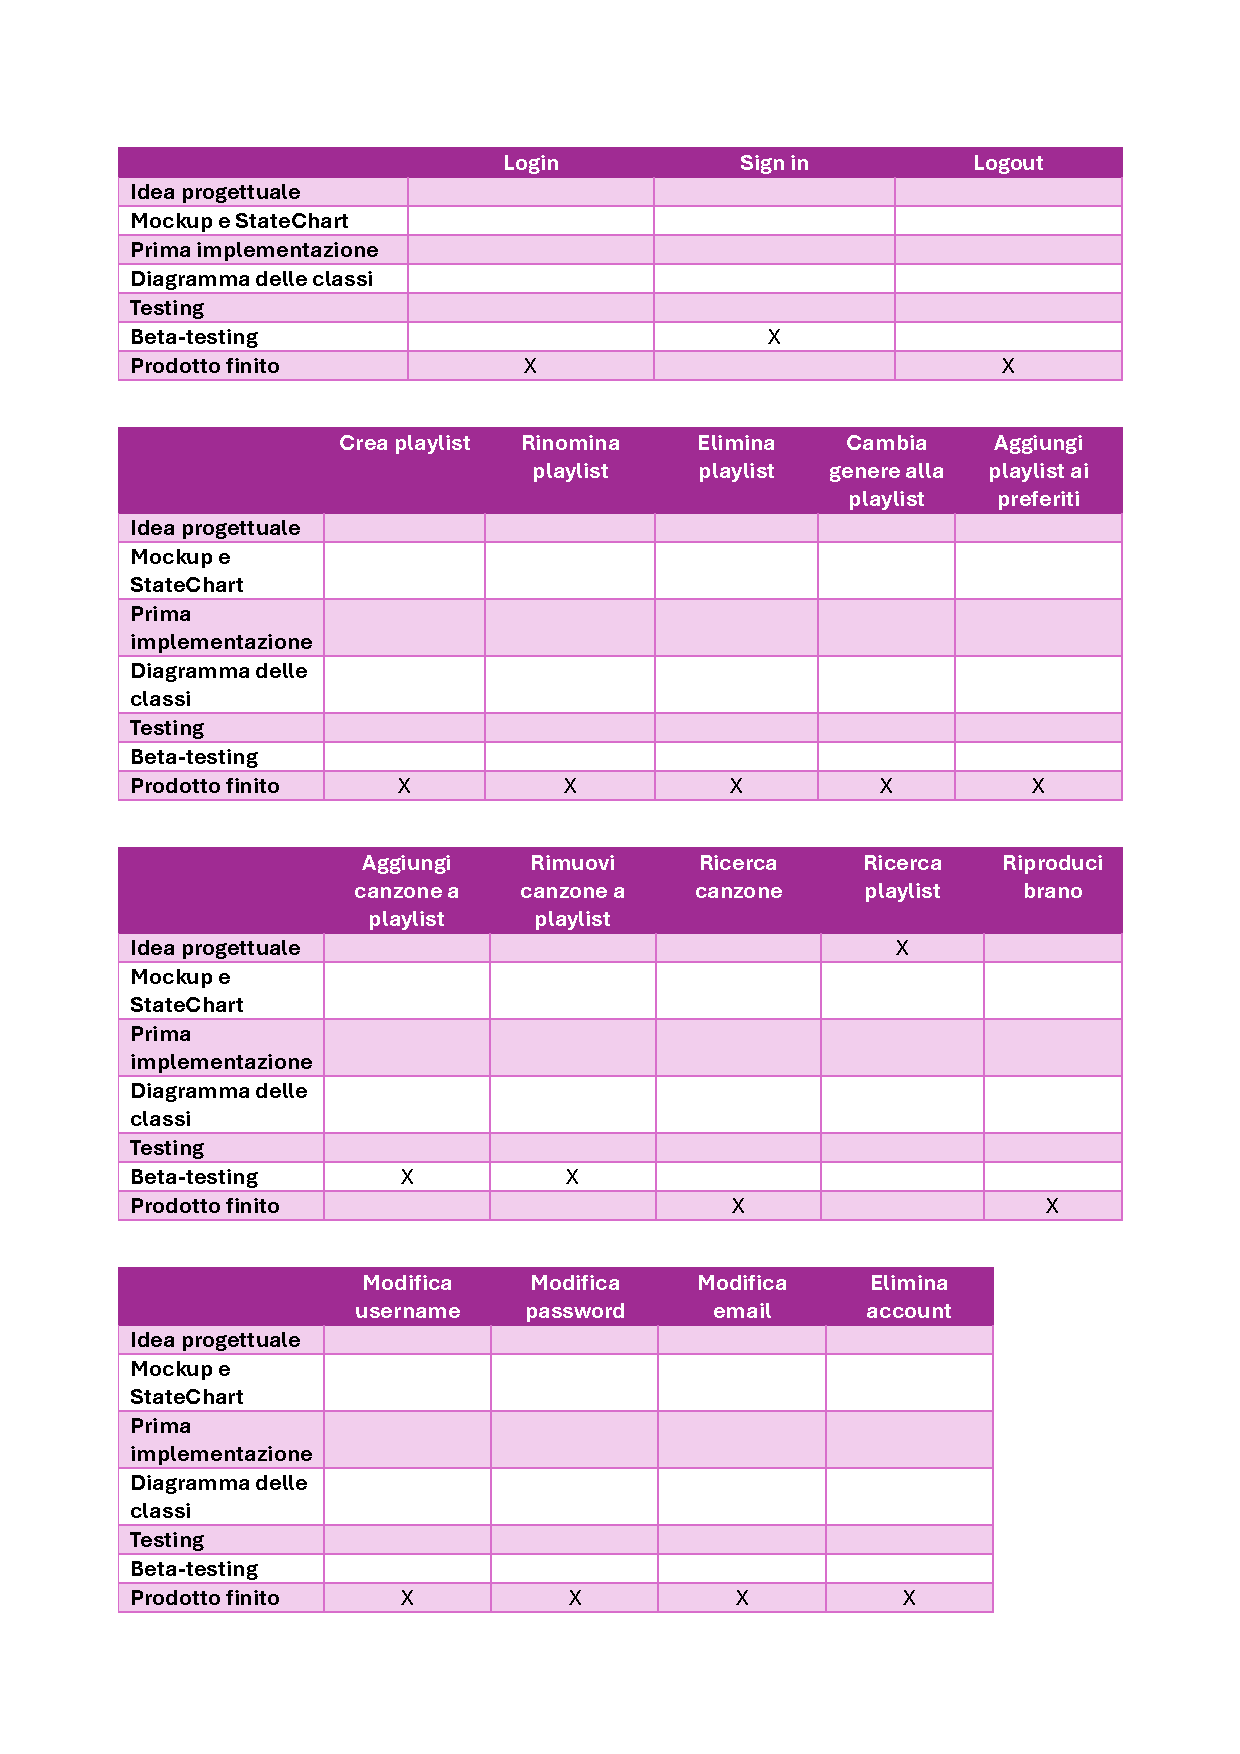
\includepdf[pages={1,2}]{Documenti/tabelle.pdf}
		\subsection{Individuazione del target di utenti}
		Il target di utenti che si può definire da una prima (e relativa) analisi dei casi d’uso sono ovviamente:
		\begin{itemize}
			\item Utenti appassionati di musica
			\item Utenti che utilizzano piattaforme digitali
			\item Utenti interessati alla personalizzazione della loro esperienza musicale
		\end{itemize}
		Dal periodo della pandemia, l'utilizzo delle piattaforme di streaming musicale ha registrato un aumento significativo. Le persone hanno cercato nuovi modi per intrattenersi a casa, e lo streaming musicale è diventato una delle attività principali.\\
		Secondo i dati, nel 2021, la media settimanale di ascolto di musica era di 18,4 ore, rispetto alle 18 ore del 2019 e alle 17,8 ore del 2018 \textbf{(Gadget Advisor)}. Questo incremento è dovuto in gran parte alla crescita delle piattaforme di streaming musicale come Apple Music e Spotify, che hanno visto un aumento significativo nel numero di utenti e nel tempo di ascolto. Ad esempio, nel primo trimestre del 2023, sono stati superati un trilione di stream audio in soli tre mesi \textbf{(Gadget Advisor)}.\\
		Le statistiche mostrano che quasi il 40\% degli utenti di età compresa tra 35 e 64 anni ha utilizzato servizi di streaming musicale nell'ultimo mese, con una crescita particolarmente forte tra le generazioni più giovani, come i Millennial e la Generazione Z \textbf{(Comparitech)}.\\ Queste fasce d'età sono le più propense a sottoscrivere abbonamenti a servizi di streaming musicale per godere di un'esperienza senza pubblicità, la possibilità di scegliere la musica da ascoltare e l'accesso a vaste librerie di brani \textbf{(Comparitech)}.\\
		L'industria della musica in streaming ha visto una crescita continua negli ultimi anni. \\Nel 2022, il numero di brani ascoltati in streaming negli Stati Uniti ha raggiunto 1,3 trilioni, un aumento del 12,2\% rispetto all'anno precedente \textbf{(Comparitech)}. Inoltre, il mercato globale dello streaming musicale è cresciuto del 10,3\% nello stesso anno, segnando l'ottavo anno consecutivo di crescita per l'industria musicale \textbf{(Comparitech)}.\\
		Questi dati evidenziano come la pandemia abbia accelerato l'adozione e l'uso delle piattaforme di streaming musicale, che continuano a crescere grazie alla crescente domanda di contenuti musicali on-demand da parte di un pubblico sempre più ampio e diversificato.
			\subsubsection{Definizione delle Personas}
			Lo studio delle \textbf{"personas"}, ovvero dei profili ideali di utenti, è fondamentale per comprendere gli elementi chiave dell'applicazione e orientare al meglio le sue funzionalità per soddisfare i desideri degli utenti.\\Nel nostro caso specifico, il focus per individuare le user-personas è stata la fascia d'età, individuando quattro categorie principali:
			
			\begin{itemize}
				\item \textbf{Gen Z:} età compresa tra i 10-23 anni
				\item \textbf{Millenials:} età compresa tra i 24-39 anni
				\item \textbf{oltre i 40 anni}
				\item \textbf{oltre i 60 anni}
			\end{itemize}
			
			\begin{center}
				\begin{figure}[H]
					\centering
					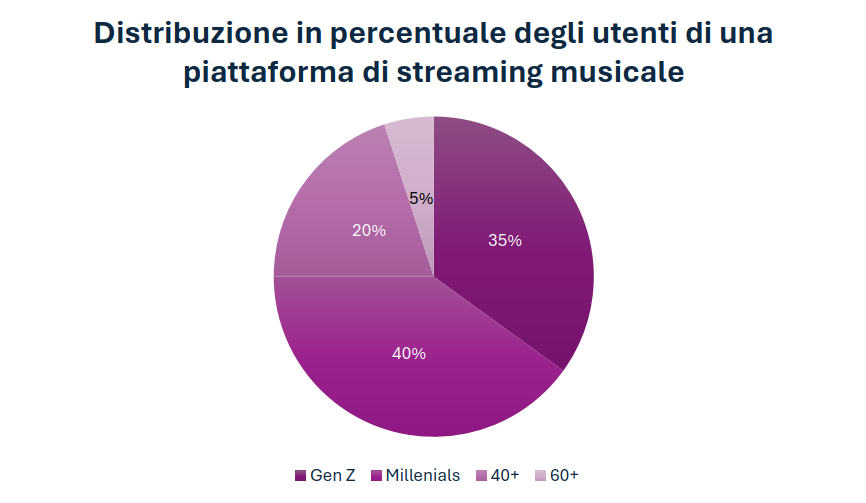
\includegraphics[width=0.9\textwidth]{Immagini/dati.png}
				\end{figure}
			\end{center}
			Di seguito, verranno illustrate le \textit{personas} ideate sulla base di quanto descritto.
			\begin{itemize}
				\item \textbf{Personas 1:} La prima user-persona appartiene alla fascia d'età denominata come Gen-Z. Studenti amanti della musica e della tecnologia che rappresentano la nuova generazione di utenti online.
				\item \textbf{Personas 2:} La seconda user-persona appartiene alla fascia d'età denominata come Millenials. Persone più affini alla tecnologia che sono appassionati di musica e che sono riusciti a farne di esse un mestiere o un'allegra compagna durante le giornate.
				\item \textbf{Personas 3:} L'ultima user-persona appartiene al range d'età più estremo che abbiamo individuato. Questa classe prevede persone che non sono esperte di tecnologia ma che vivono della loro passione.
			\end{itemize}
			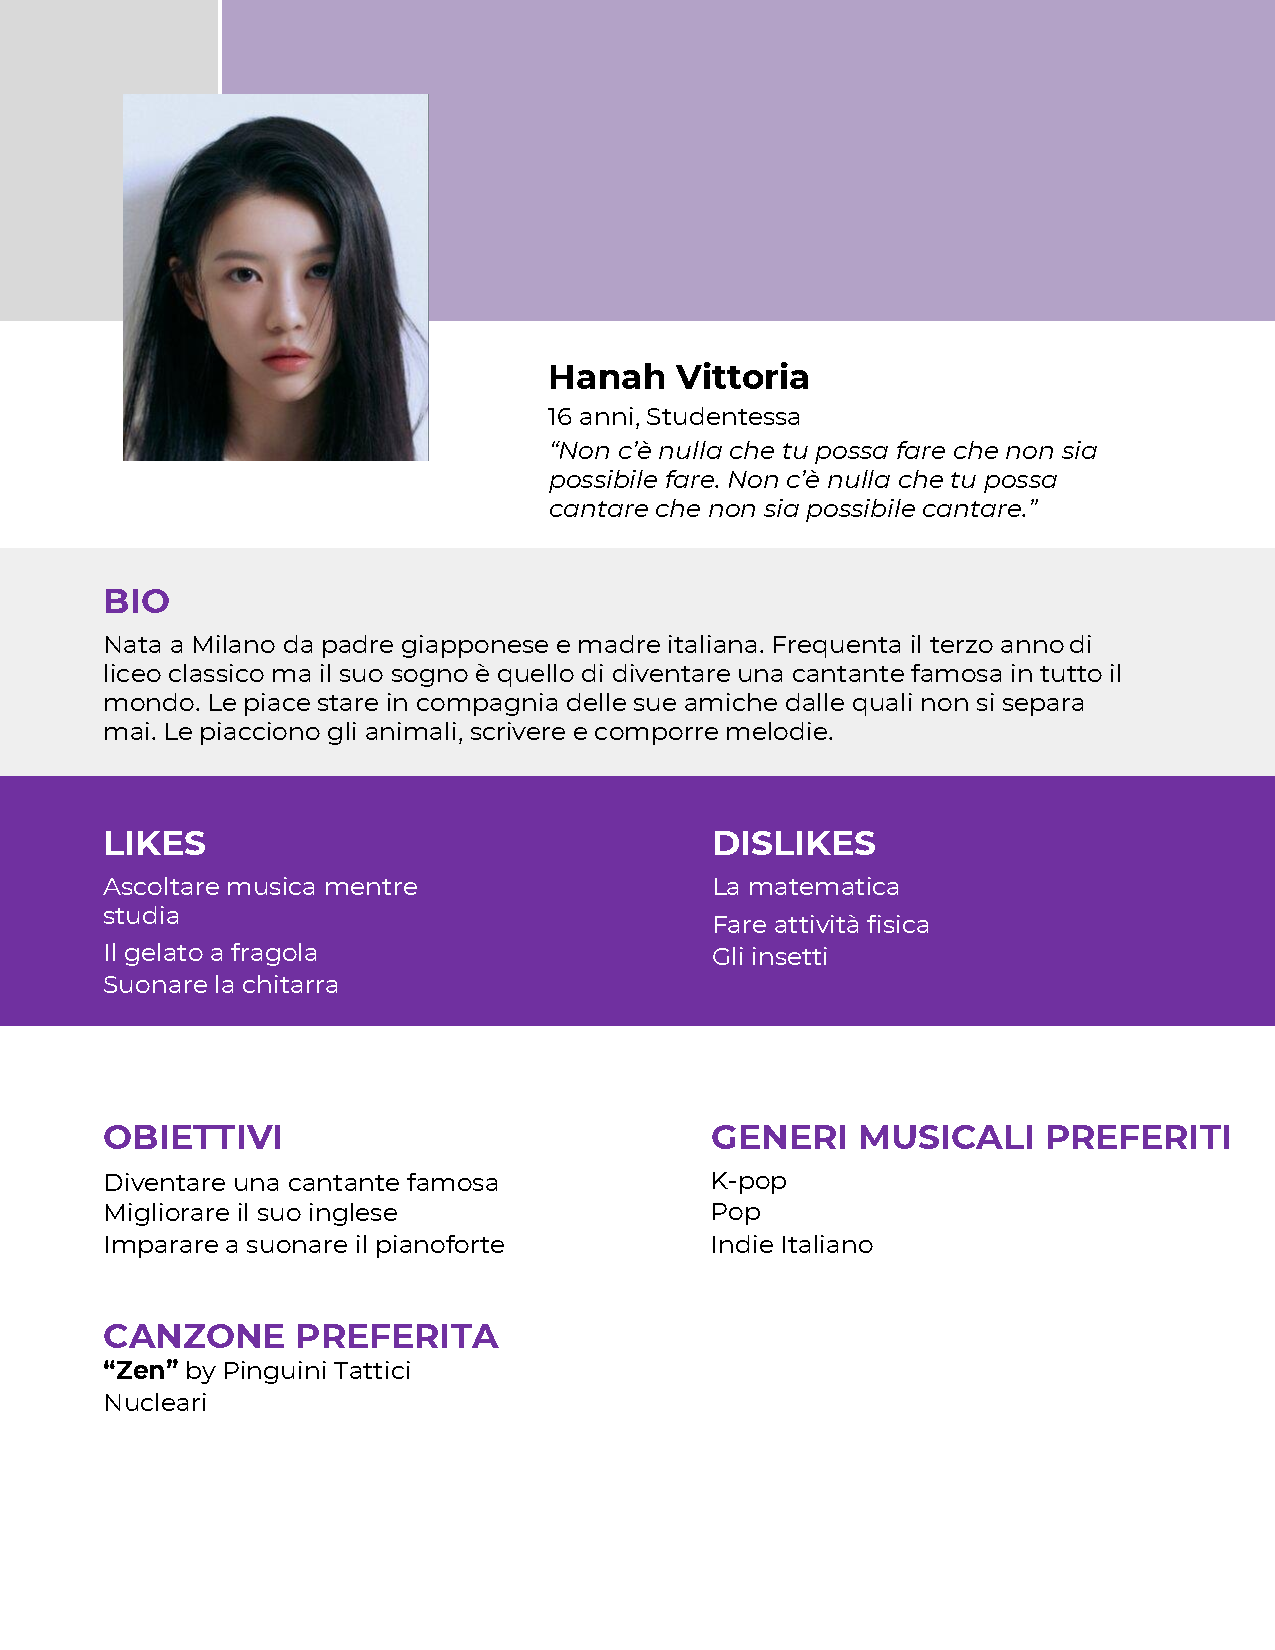
\includepdf[keepaspectratio]{Documenti/UserPersona1}
			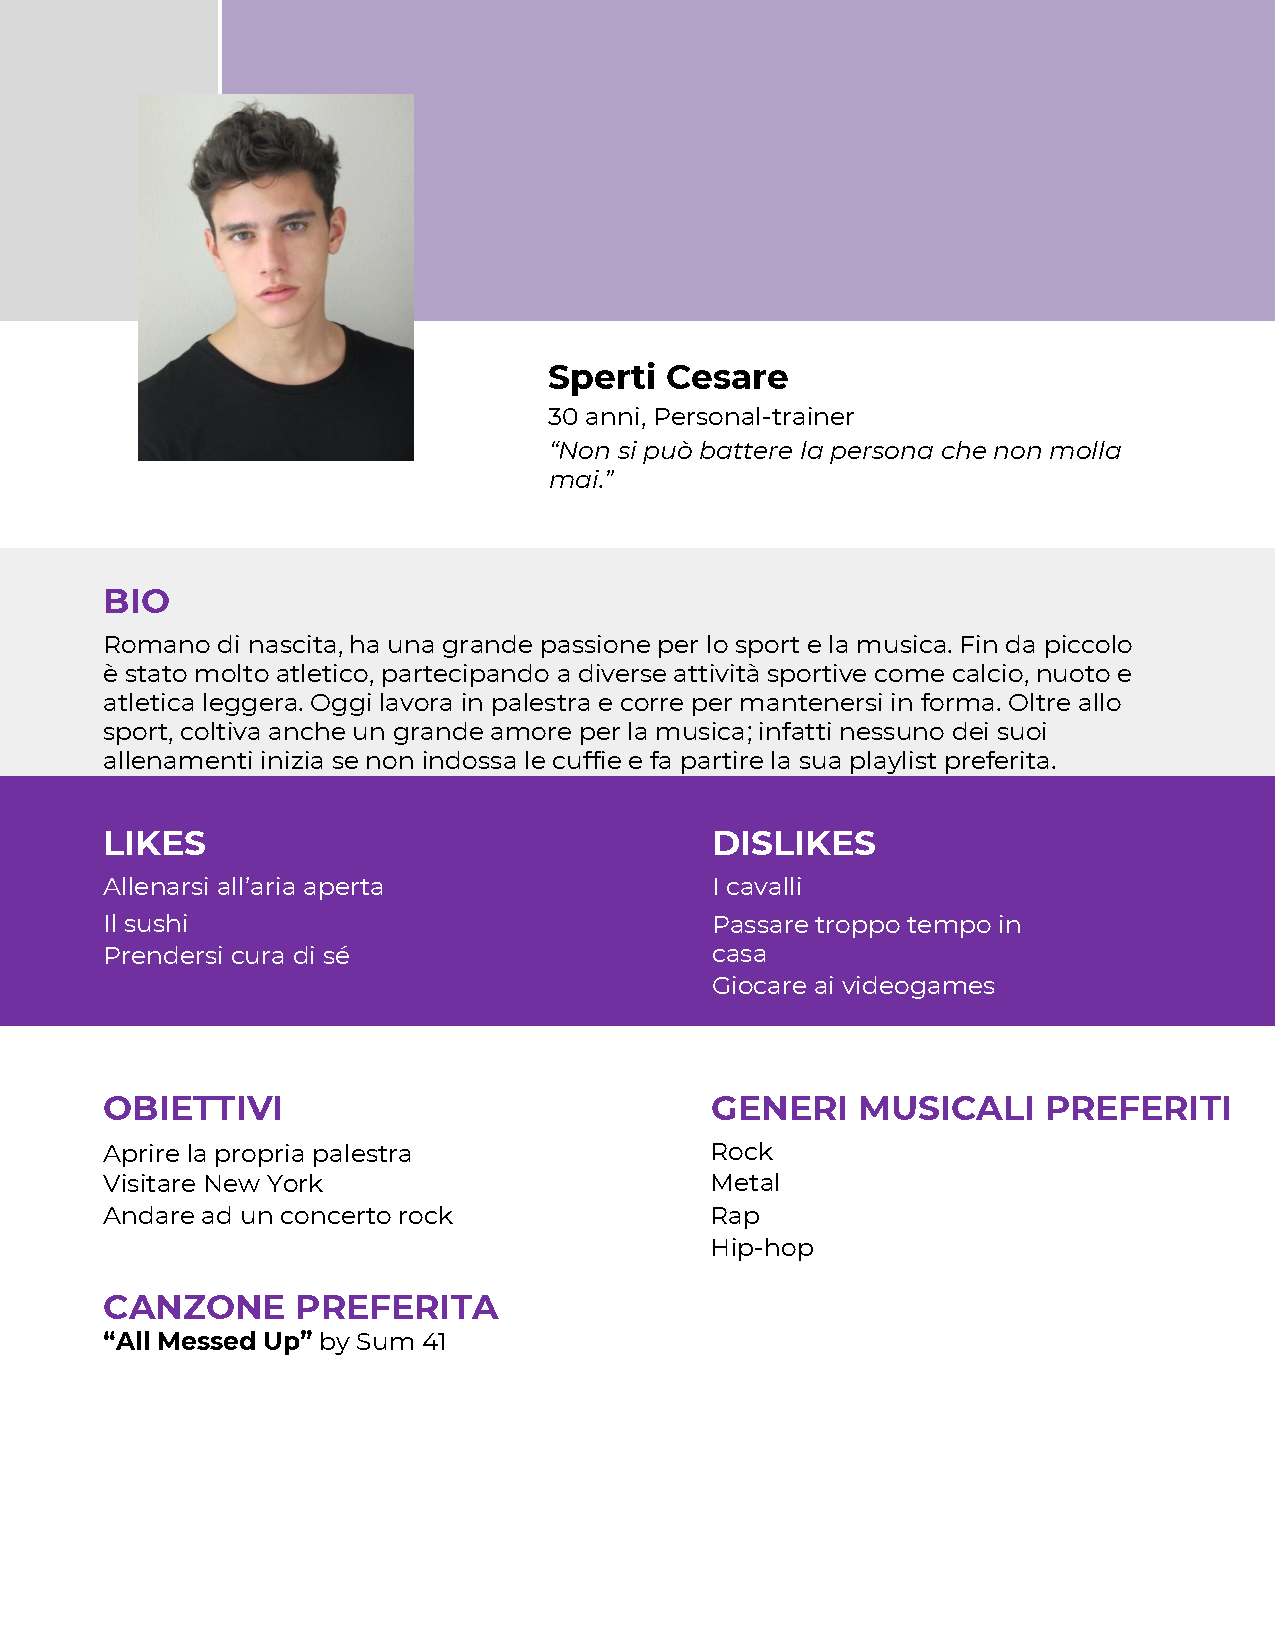
\includepdf[keepaspectratio]{Documenti/UserPersona2.pdf}
			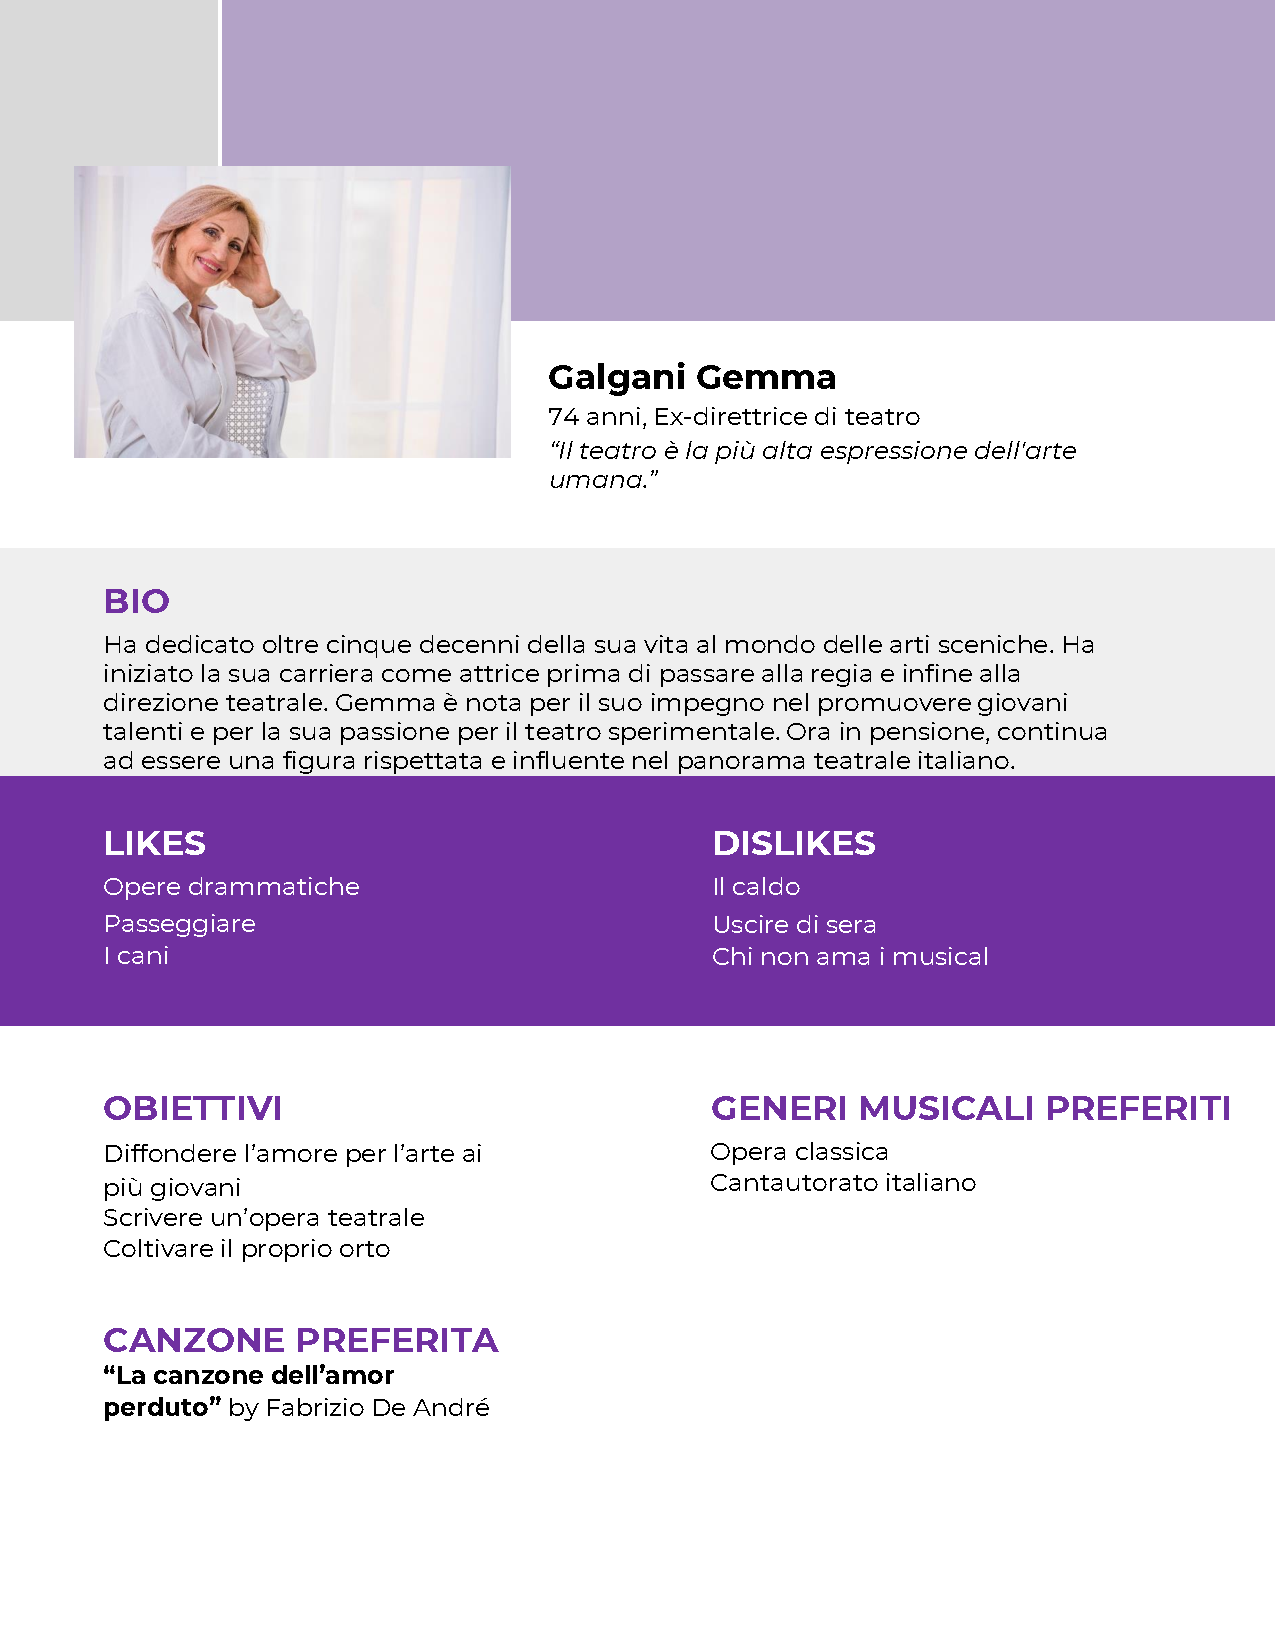
\includepdf[keepaspectratio]{Documenti/UserPersona3.pdf}
				
		\subsection{Valutazione dell'usabilità a priori}
		Per ottenere una valutazione dell'usabilità a priori più corretta possibile, si è cercato di riprodurre dei prototipi avendo le idee ben chiare sull'aspetto e sulle funzionalità che doveva avere l'applicativo. Si è deciso di restare il più fedeli possibile ai prototipi così da avere una valutazione a priori quanto più vicina a quella a posteriori in beta-testing.
		I mockup sono stati realizzati su \textbf{Figma} che consente di realizzare rapidamente prototipi interattivi, permettendo di testare e iterare facilmente le idee con gli stakeholder.
		È più semplice progettare interfacce accessibili e responsive utilizzando i potenti strumenti di layout e tipografia di Figma.\\
		I mockup, e soprattutto l’app, sono stati realizzati seguendo \textbf{le 8 regole d’oro di Shneiderman}.\\
		\textit{NOTA: I punti evidenziati sono quelli sui quali è stata posta più attenzione.}
		\begin{itemize}
			\item \textbf{Coerenza a tutti i costi}
			\item \textbf{Usabilità universale}
			\item Offrire riscontri informativi
			\item Dialogo con gli utilizzatori
			\item \textbf{Prevenire gli errori}
			\item Assicurare la reversibilità
			\item \textbf{Garantire il controllo degli utenti}
			\item \textbf{Ridurre il carico di memoria a breve termine}
		\end{itemize}
			\subsubsection{Tabelle di valutazione e tecniche utilizzate}
			Precedentemente sono state chiarite le motivazioni dietro le scelte fatte in termini di design di UI e UX per l’applicativo. Pur ritenendo queste le migliori scelte, è altrettanto importante ottenere un feedback anche dai futuri utenti.
			Si è scelto quindi di fare una valutazione a priori dell’usabilità dell’applicativo, rispettando \textbf{le regole di Nielsen}\footnote{https://aelaschool.com/en/interactiondesign/10-usability-heuristics-ui-design/}.
			Sono stati selezionati \textbf{cinque candidati} ai quali è stato richiesto di eseguire \textbf{cinque task}, con pochissime indicazioni da parte del team.
			\begin{itemize}
				\item Registrazione di un account
				\item Creazione di una playlist
				\item Aggiunta di una canzone ad una playlist
				\item Modifica password
				\item Ricerca di un brano musicale
			\end{itemize}
			La scelta dei candidati è stata invece fatta sulla base della loro età e delle loro competenze digitali.
			Questi ultimi due valori saranno classificati in tale modo:
			\begin{itemize}
				\item \textbf{Naive:} useremo \textbf{N} per indicare ciò
				\item \textbf{Abile:} useremo \textbf{A} per indicare ciò
				\item \textbf{Esperto:} useremo \textbf{E} per indicare ciò
			\end{itemize}
			L’eventuale riuscita o meno delle task sarà segnata invece come:
			\begin{itemize}
				\item \textbf{F:} per indicare che la task non è stata completata
				\item \textbf{S:} per indicare che la task è stata completata con successo
				\item \textbf{//:} per indicare che la task è stata portata a termine, ma il candidato ha avuto bisogno di qualche aiuto in più su come procedere
			\end{itemize}
			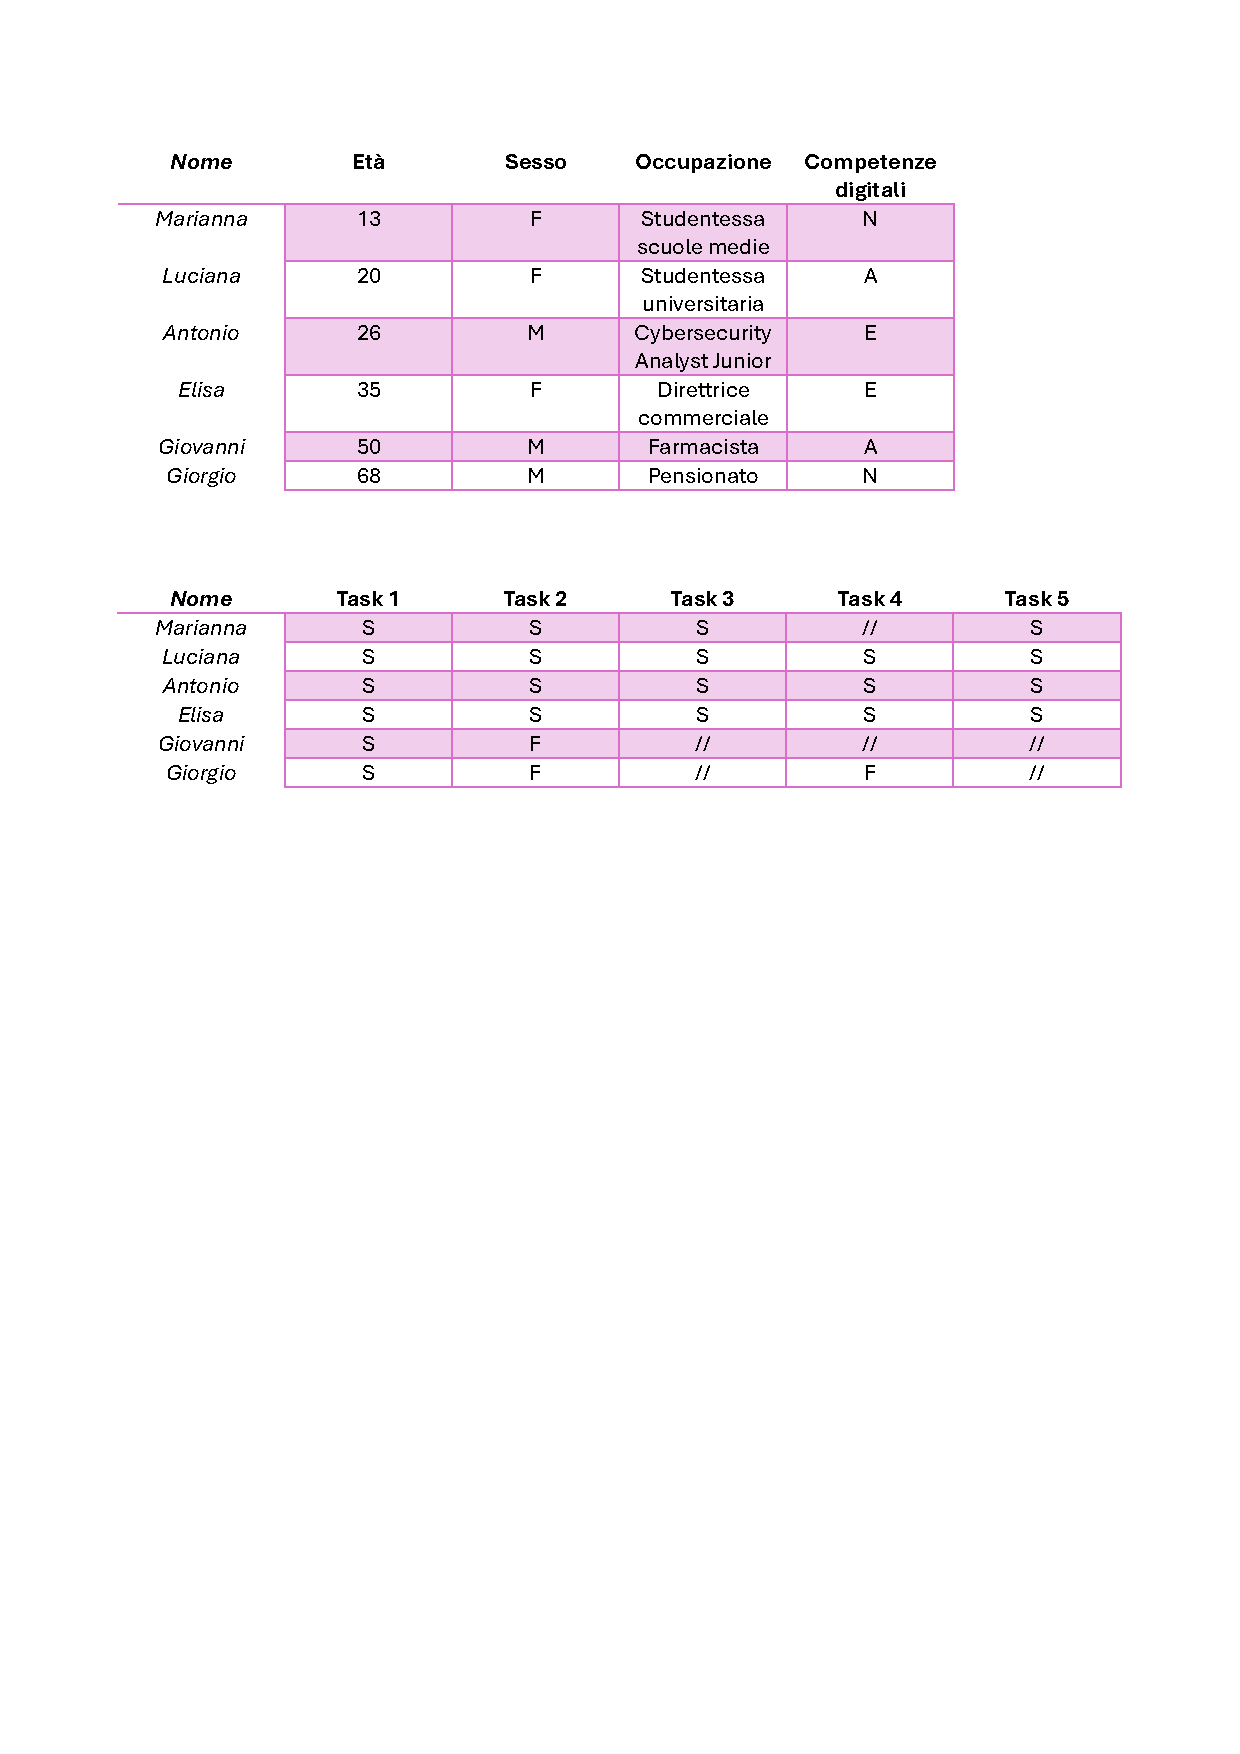
\includepdf[keepaspectratio]{Documenti/tabelleutenti}
			In generale si è piuttosto soddisfatti dei risultati. I candidati hanno tutti concordato sulla generale intuitività dell’interfaccia grafica e il numero di fallimenti è stato piuttosto limitato. 
			Molto importante per il team è stato soprattutto notare come i due candidati adulti siano riusciti comunque a stabilire più successi che fallimenti, seppur necessitando spesso di conferme su quello che stavano facendo.
			\newpage
		\subsection{Prototipazione funzionale via statechart dell’interfaccia grafica}
		Di seguito vengono rappresentate mediante statechart \textbf{l'aggiunta di una playlist alle preferite} piattaforma e \textbf{l'eliminazione di una playlist}
		\begin{figure}[H]
			\centering
			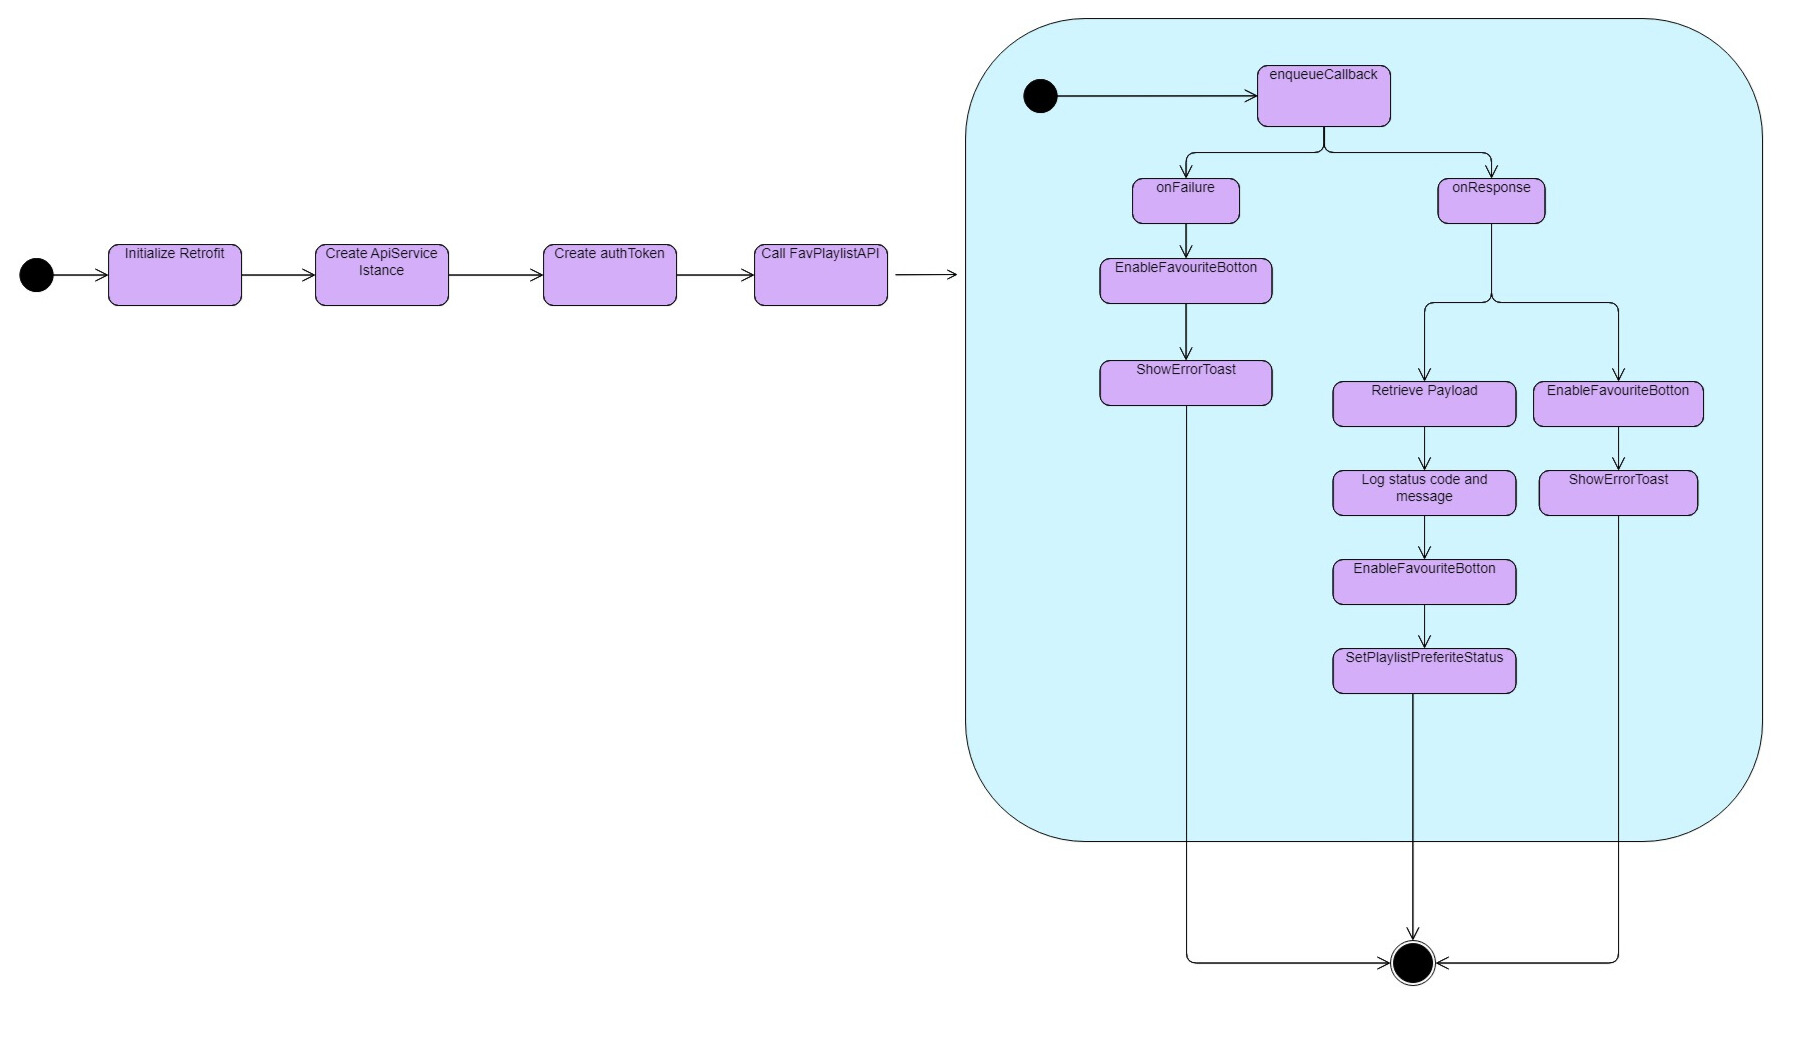
\includegraphics[width=0.9\textwidth]{Immagini/statechart1}
			\caption{Statechart Inserisci playlist ai preferiti}
		\end{figure}
		\begin{figure}[H]
			\centering
			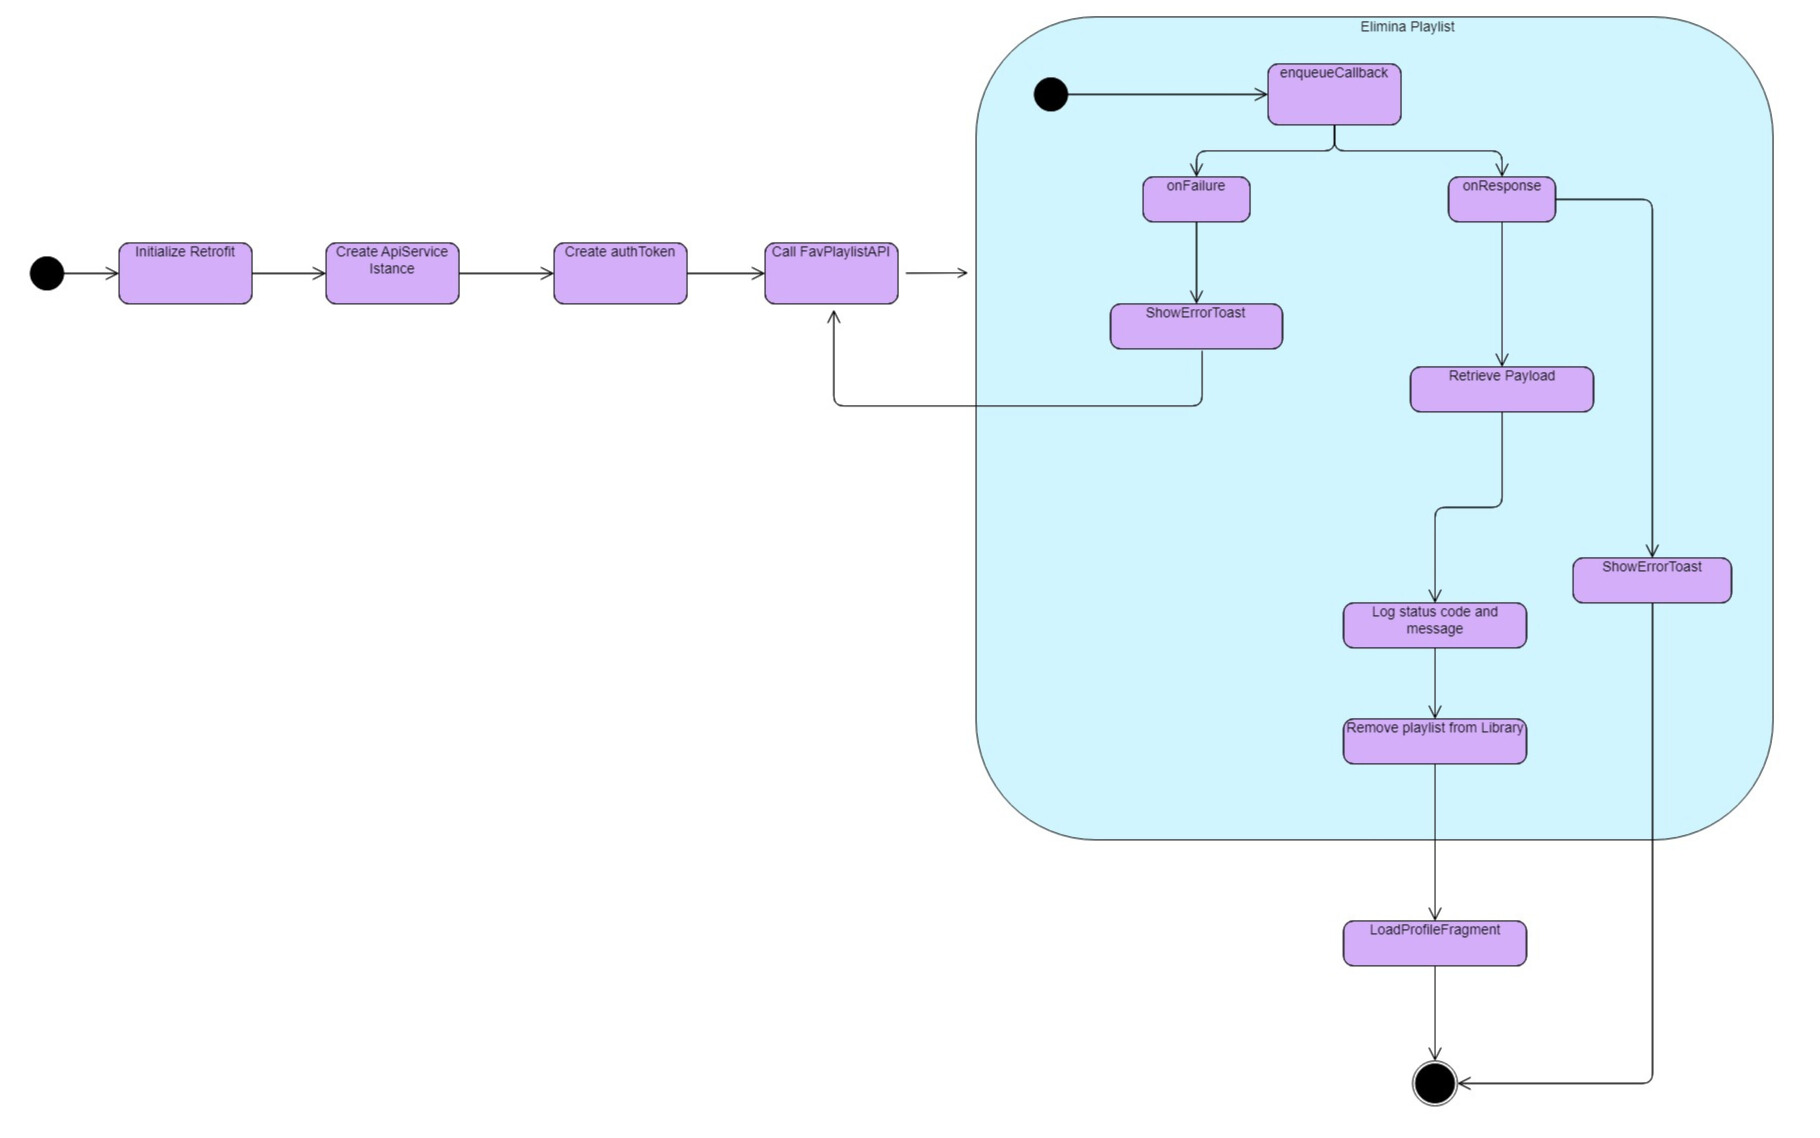
\includegraphics[width=0.9\textwidth]{Immagini/statechart2}
			\caption{Statechart Elimina playlist}
		\end{figure}
		\subsection{Glossario}
			\subsubsection{Termini}
			\begin{itemize}
				\item \textbf{\textit{\textcolor{dark_purple}{Actor}}} Nelle tabelle di Cockburn o negli Use Case Diagram, è la persona che interagisce con il sistema
				\item \textbf{\textit{\textcolor{dark_purple}{Database}}} Un archivio di dati strutturato per la memorizzazione persistente, la gestione e l’aggiornamento di informazioni utiliper il sistema
				\item \textbf{\textit{\textcolor{dark_purple}{Back-end}}} Parte di sviluppo che non opera sul client e che fornisce unservizio.
				\item \textbf{\textit{\textcolor{dark_purple}{Android}}} Sistema operativo mobile
				\item \textbf{\textit{\textcolor{dark_purple}{Mockup}}} È una rappresentazione grafica a scopo illustrativo di un oggetto o un sistema. Nel nostro caso, l’uso dei mock-up è funzionale a mostrare il funzionamento di specifiche interazioni col sistema
				\item \textbf{\textit{\textcolor{dark_purple}{Tabelle di Cockburn}}} Descrizione in linguaggio naturale delle azioni necessarie all’esecuzione di un caso d’uso
				\item \textbf{\textit{\textcolor{dark_purple}{Use Case}}} La rappresentazione di un’astrazione che descrive una classe di scenario del sistema
				\item \textbf{\textit{\textcolor{dark_purple}{Statechart}}} Un diagramma per descrivere il comportamento di entità o di classi in termini di stato (macchina a stati
				\item \textbf{\textit{\textcolor{dark_purple}{UX Design}}} Tutto ciò che afferisce l’interazione tra una persona con un prodotto, un servizio o un sistema
				\item \textbf{\textit{\textcolor{dark_purple}{Classe}}} Nella programmazione orientata a oggetti, una classe fa riferimento a un insieme di oggetti con proprietà comuni.
				\item \textbf{\textit{\textcolor{dark_purple}{Framework}}} Architettura logica di supporto sulla quale un software può essere progettato e realizzato, facilitandone lo sviluppo.
				\item \textbf{\textit{\textcolor{dark_purple}{Scalabilità}}} Capacità di un sistema di aumentare o diminuire di scala in funzione delle necessità.
				\item \textbf{\textit{\textcolor{dark_purple}{Usabilità}}} Il "grado in cui un prodotto può essere usato da particolari utenti per raggiungere certi obiettivi con efficacia, efficienza e soddisfazione in uno specifico contesto d’uso.
				\item \textbf{\textit{\textcolor{dark_purple}{Elasticità}}} Si riferisce alla capacità di un servizio cloud di offrire servizi su richiesta aumentando o diminuendo le risorse quando la domanda sale o scende.
			\end{itemize}
	\section{Modelli di dominio}
	In questa sezione verranno analizzati i modelli di dominio dell'applicazione ancora in fase di analisi dei requisiti.
	In particolare utilizzeremo per tale analisi:
	\begin{itemize}
		\item \textbf{Class Diagram}
		\item \textbf{Sequence Diagram}
		\item \textbf{Diagramma di attività}
	\end{itemize}
	Per far si che ci sia una facile comprensione e per individuare classi ed entità in gioco è stata ritenuta fondamentale l’euristica\textbf{ Three Object-Type} o anche conosciuta con tre acronimi:
	\begin{itemize}
		\item \textbf{ Entity:} entità o modelli che sono in gioco
		\item \textbf{Boundary:} rappresentano le interazioni tra sistema ed utente
		\item \textbf{Control:} rappresentano i controller o meglio definita la logica del sistema che si occupa di definire gli use case sotto sviluppo
	\end{itemize}
		\subsection{Classi, oggetti e relazioni di analisi}
			\subsubsection{Classi ed entità}
			Di seguito verrà riportata una rappresentazione delle entità che sono state individuate e che saranno esse stesso gli oggetti in gioco per i vari use case assegnati.
			\begin{figure}[H]
				\centering
				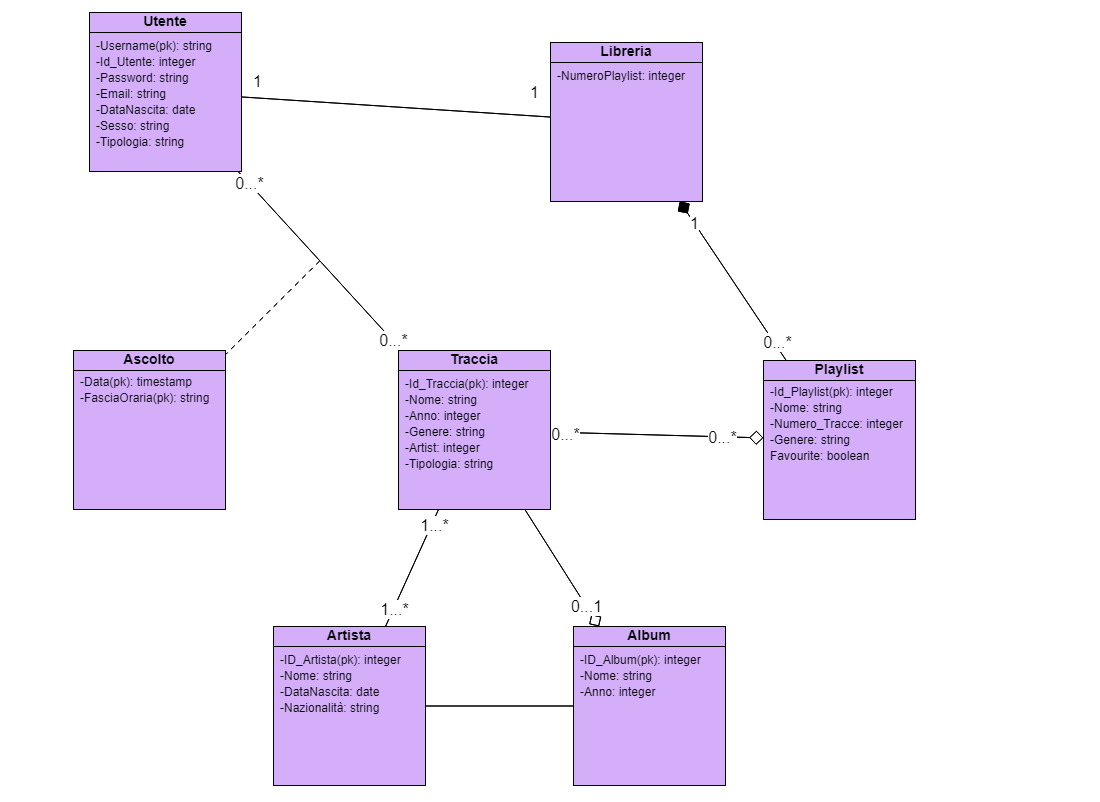
\includegraphics[width=0.9\textwidth]{Immagini/classdiagramgenerale}
				\caption{Class Diagram generale}
			\end{figure}
			\subsubsection{Class diagram delle funzionalità}
			In questa sezione elencheremo tutti i classdiagram suddivisi.\\
			\textit{NOTA: Per una questione puramente stilistica volta ad una comprensione facilitata dei class diagram, si è optato per utilizzare bianco e nero, piuttosto che il viola.}
			\begin{figure}[H]
				\centering
				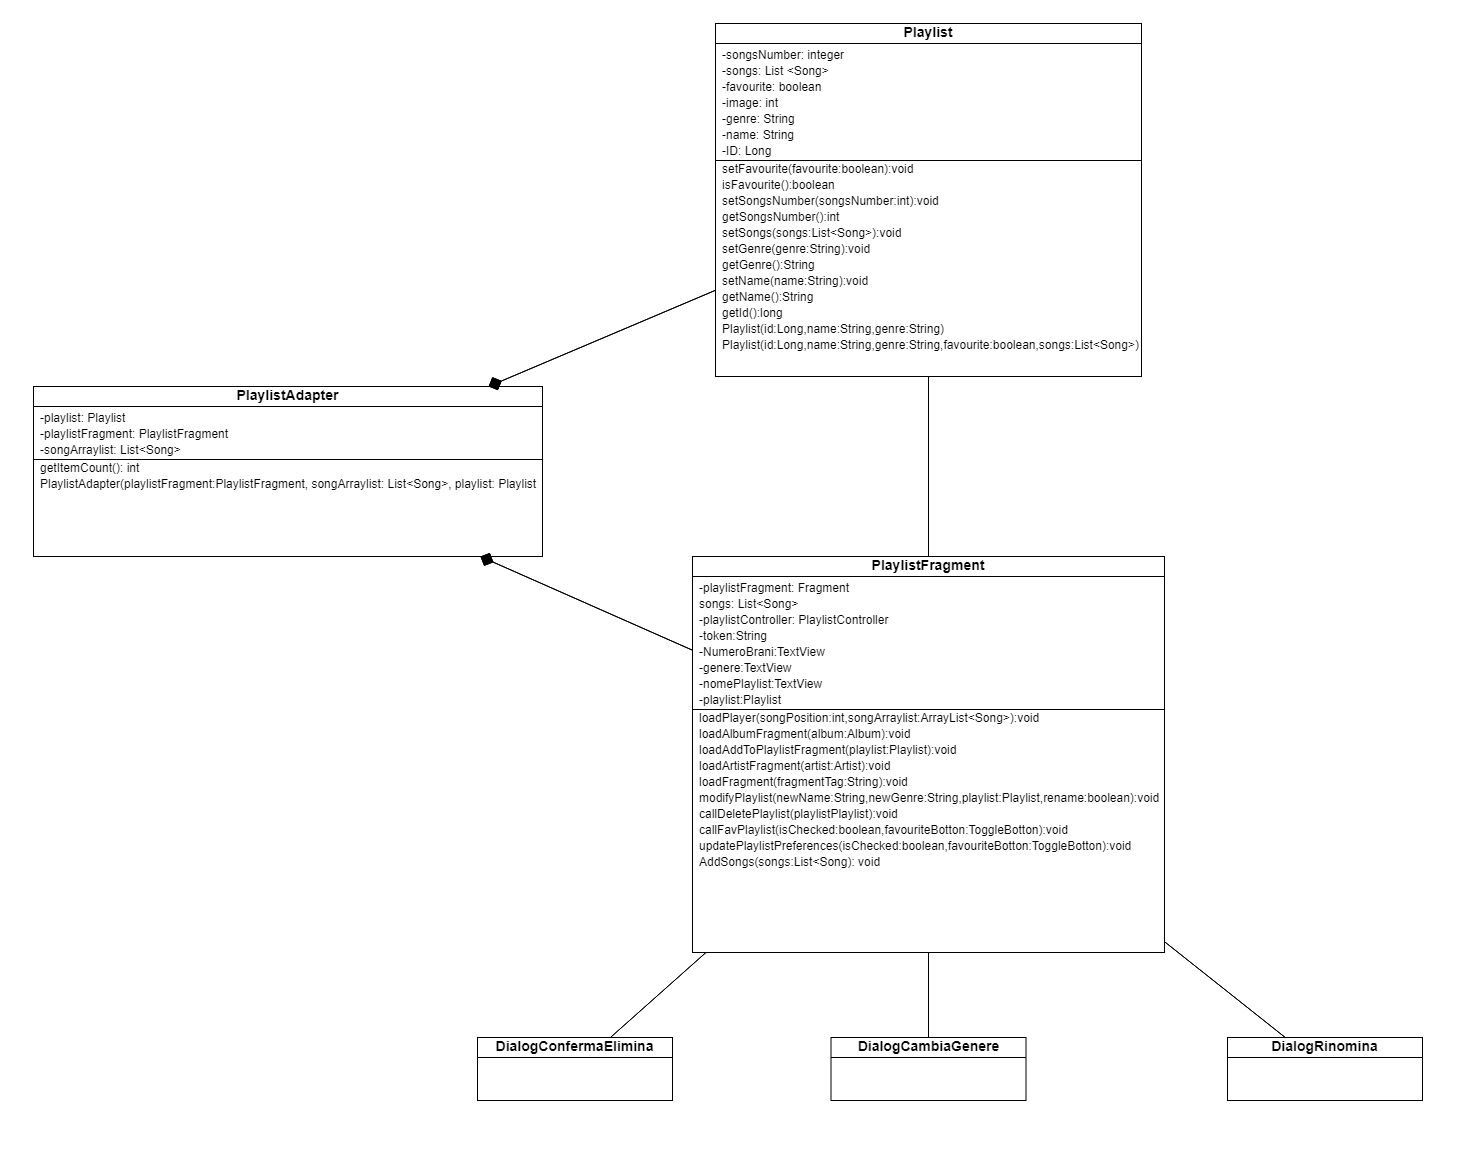
\includegraphics[width=0.9\textwidth]{Immagini/classdiagramplaylist}
				\caption{Class Diagram Playlist}
			\end{figure}
			\vspace{0.9cm}
			\begin{figure}[H]
				\centering
				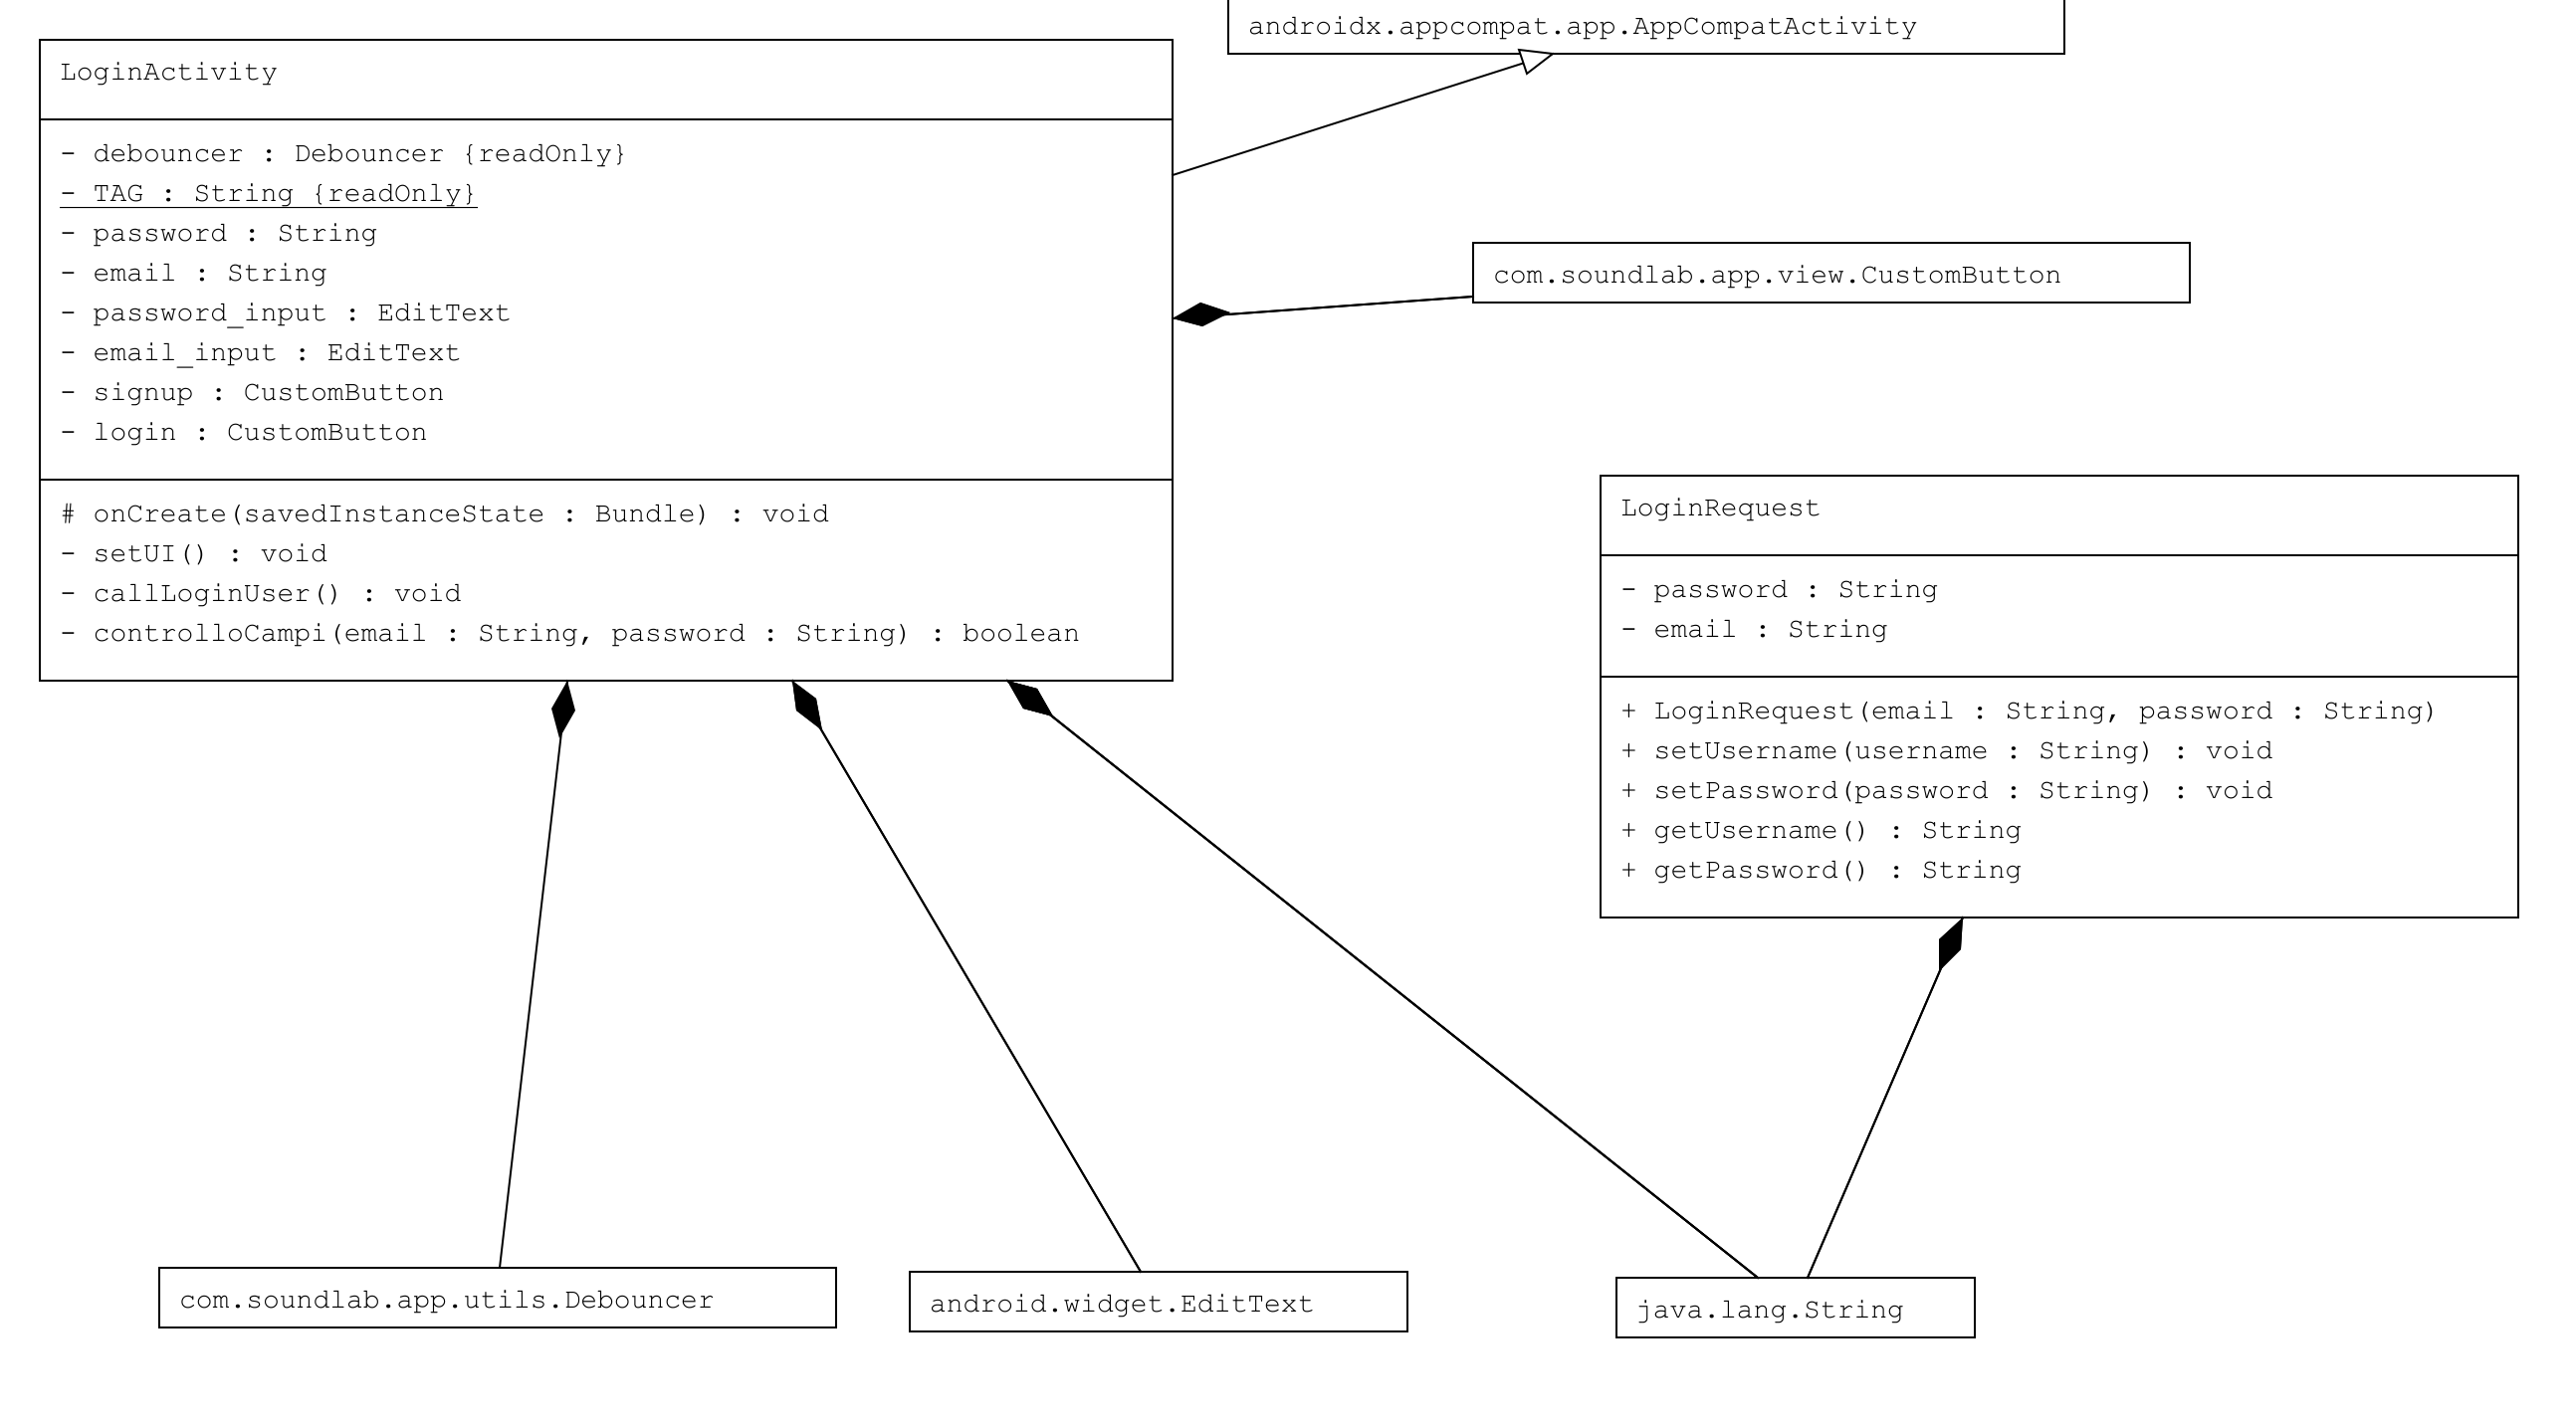
\includegraphics[width=0.9\textwidth]{Immagini/classdiagramlogin}
				\caption{Class Diagram Login}
			\end{figure}
			\vspace{0.9cm}
			\begin{figure}[H]
				\centering
				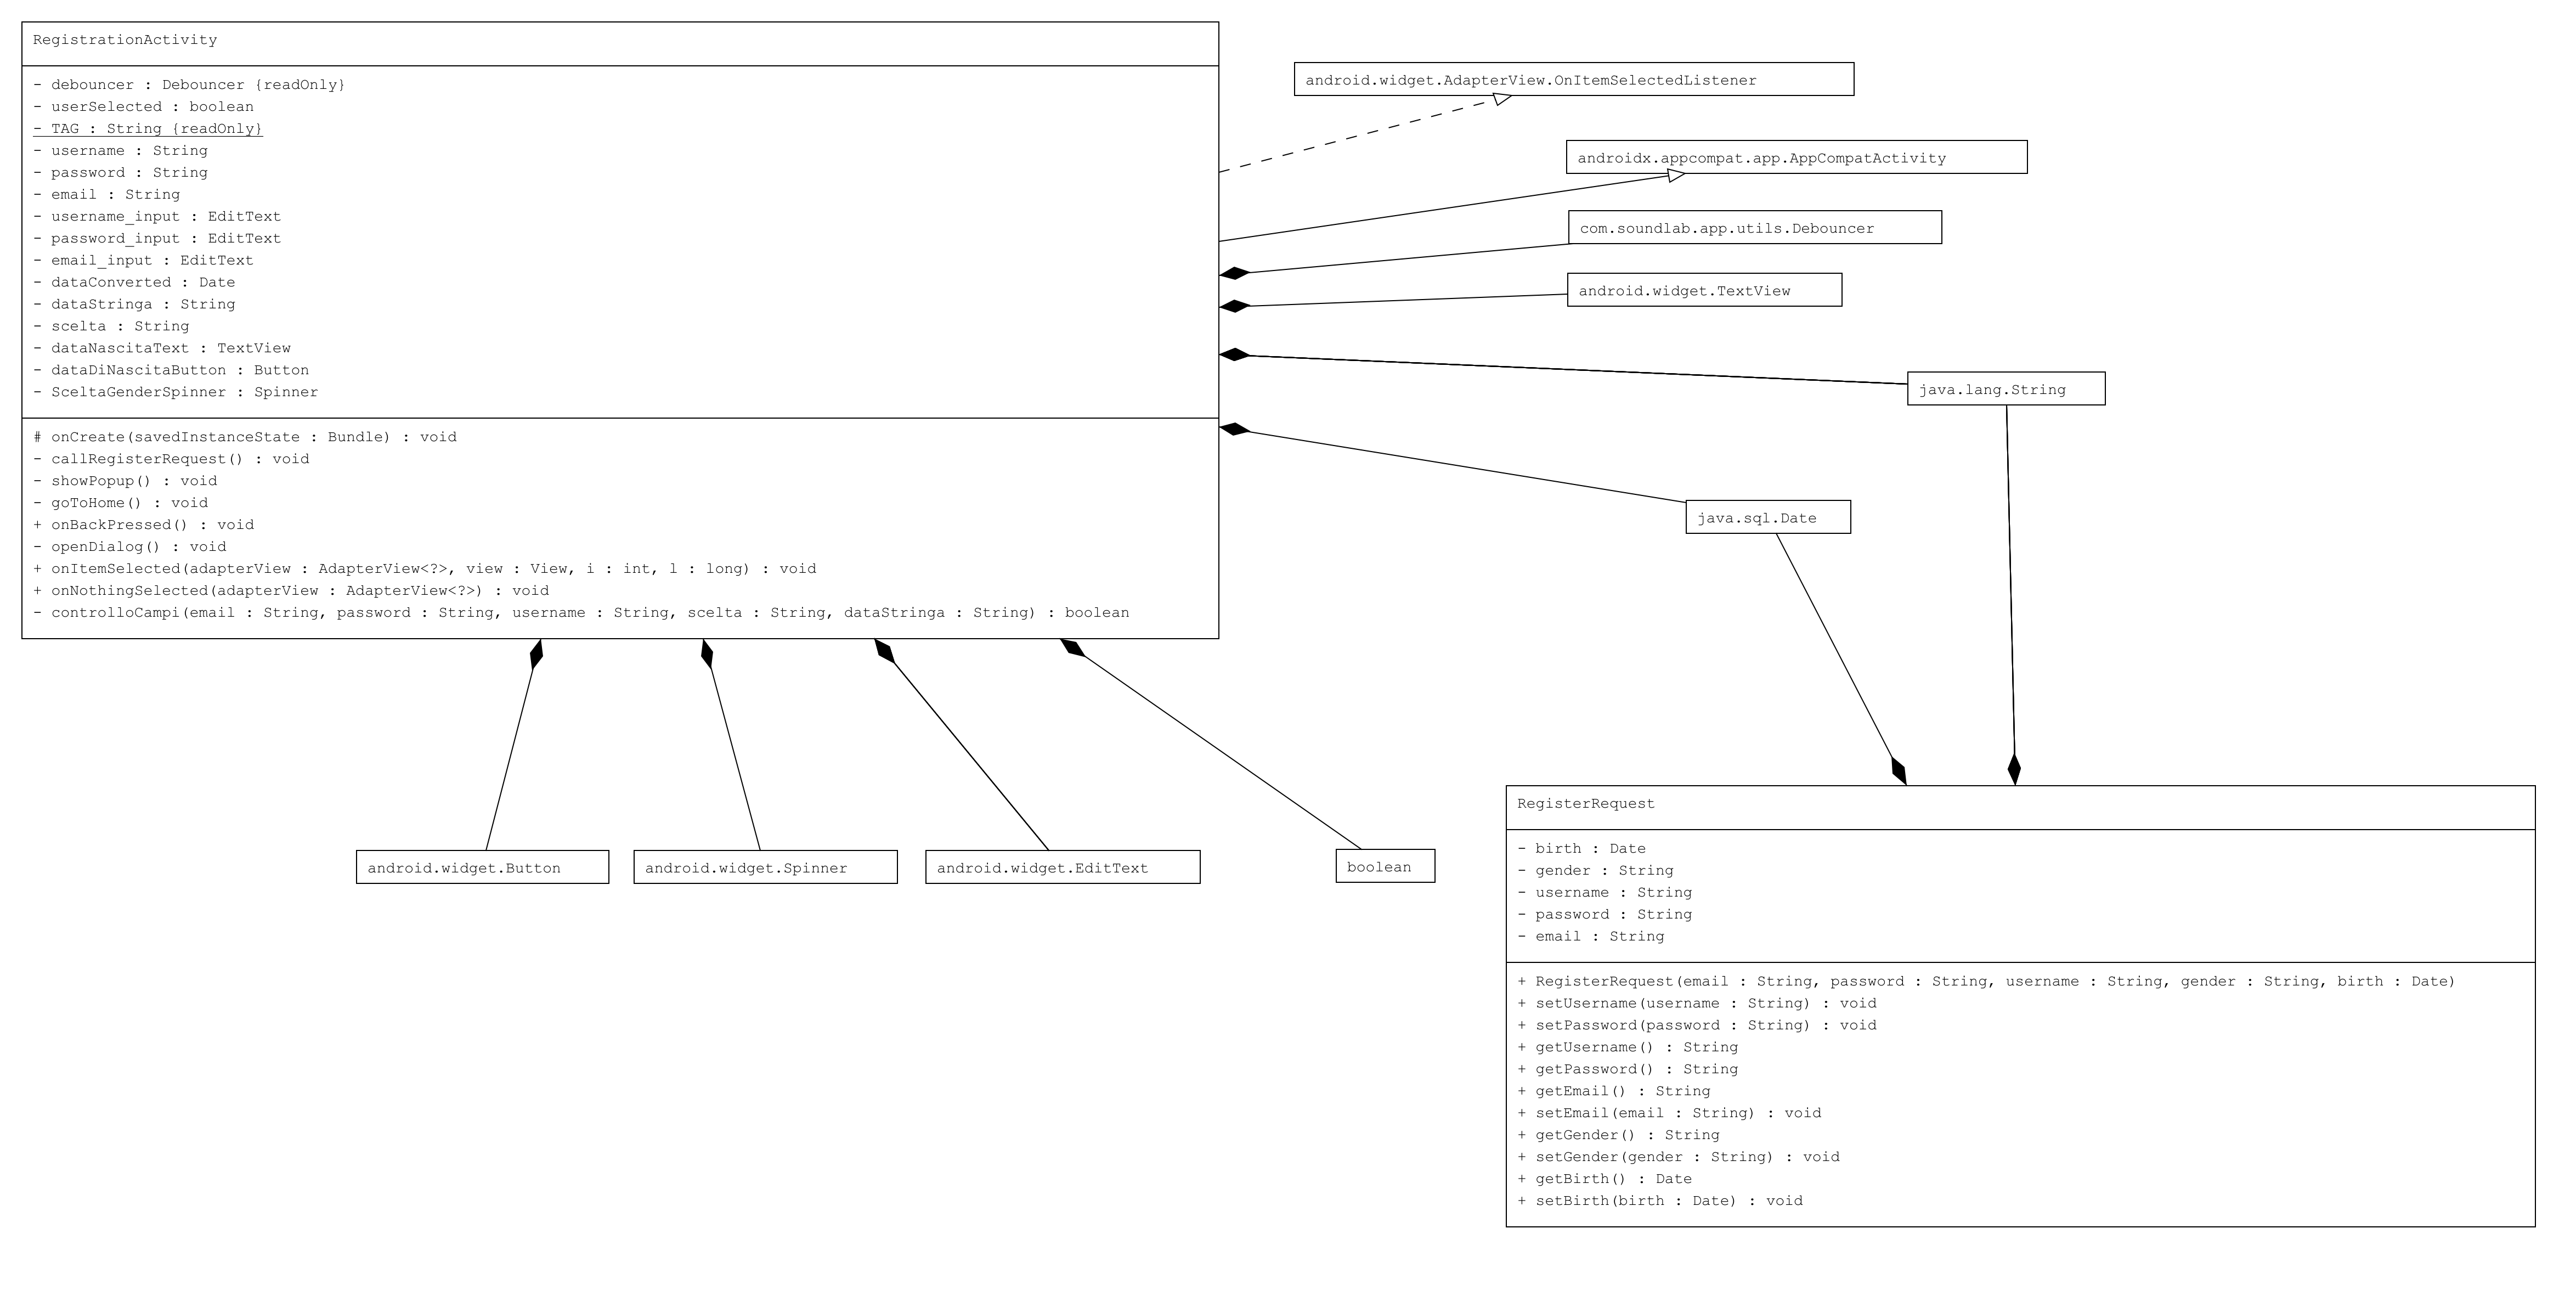
\includegraphics[width=0.9\textwidth]{Immagini/classdiagramregistrazione}
				\caption{Class Diagram Registrazione}
			\end{figure}
			\vspace{0.9cm}
			\begin{figure}[H]
				\centering
				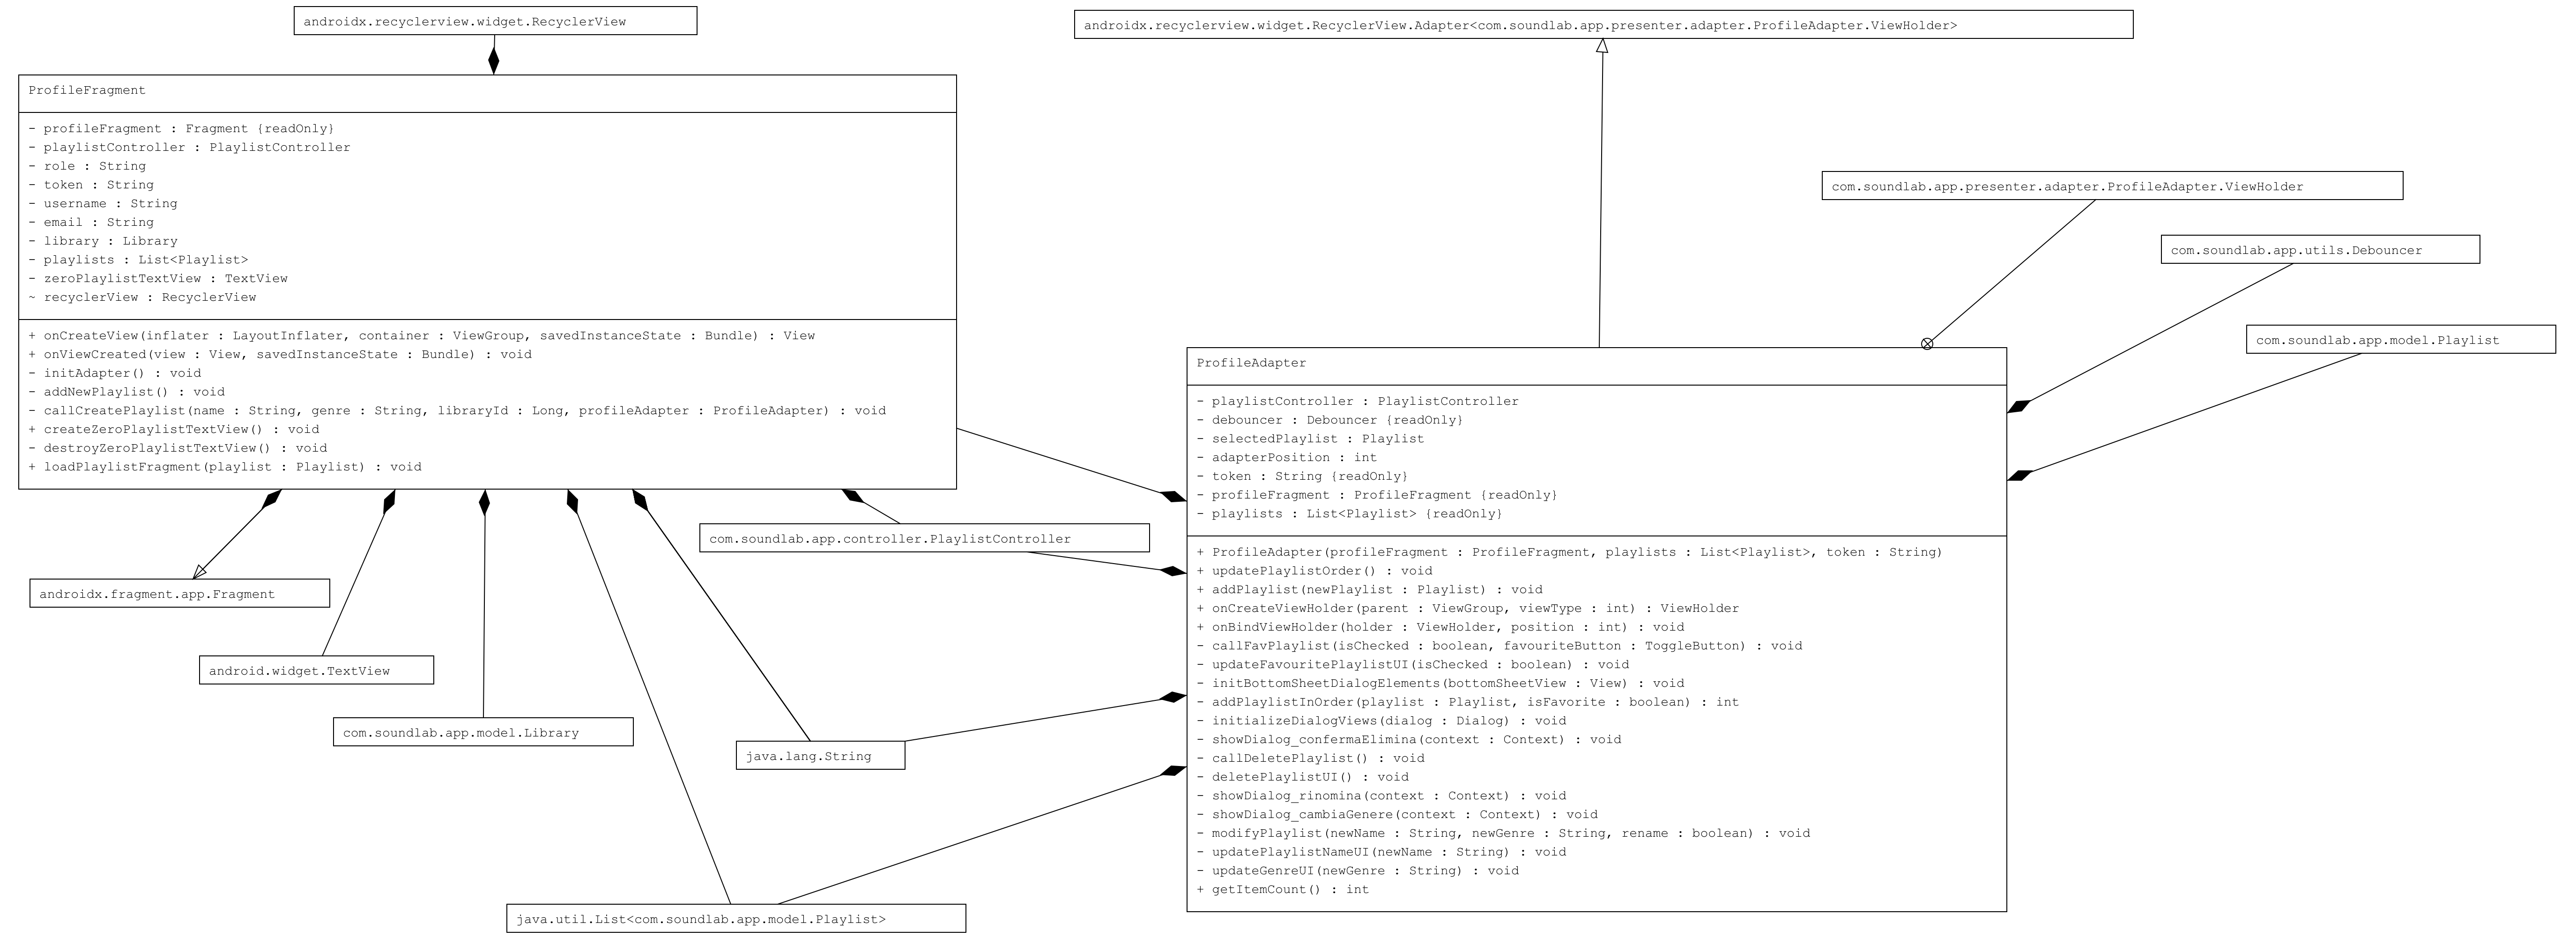
\includegraphics[width=0.9\textwidth]{Immagini/classdiagramprofilo}
				\caption{Class Diagram Profilo}
			\end{figure}
			\vspace{0.9cm}
			\begin{figure}[H]
				\centering
				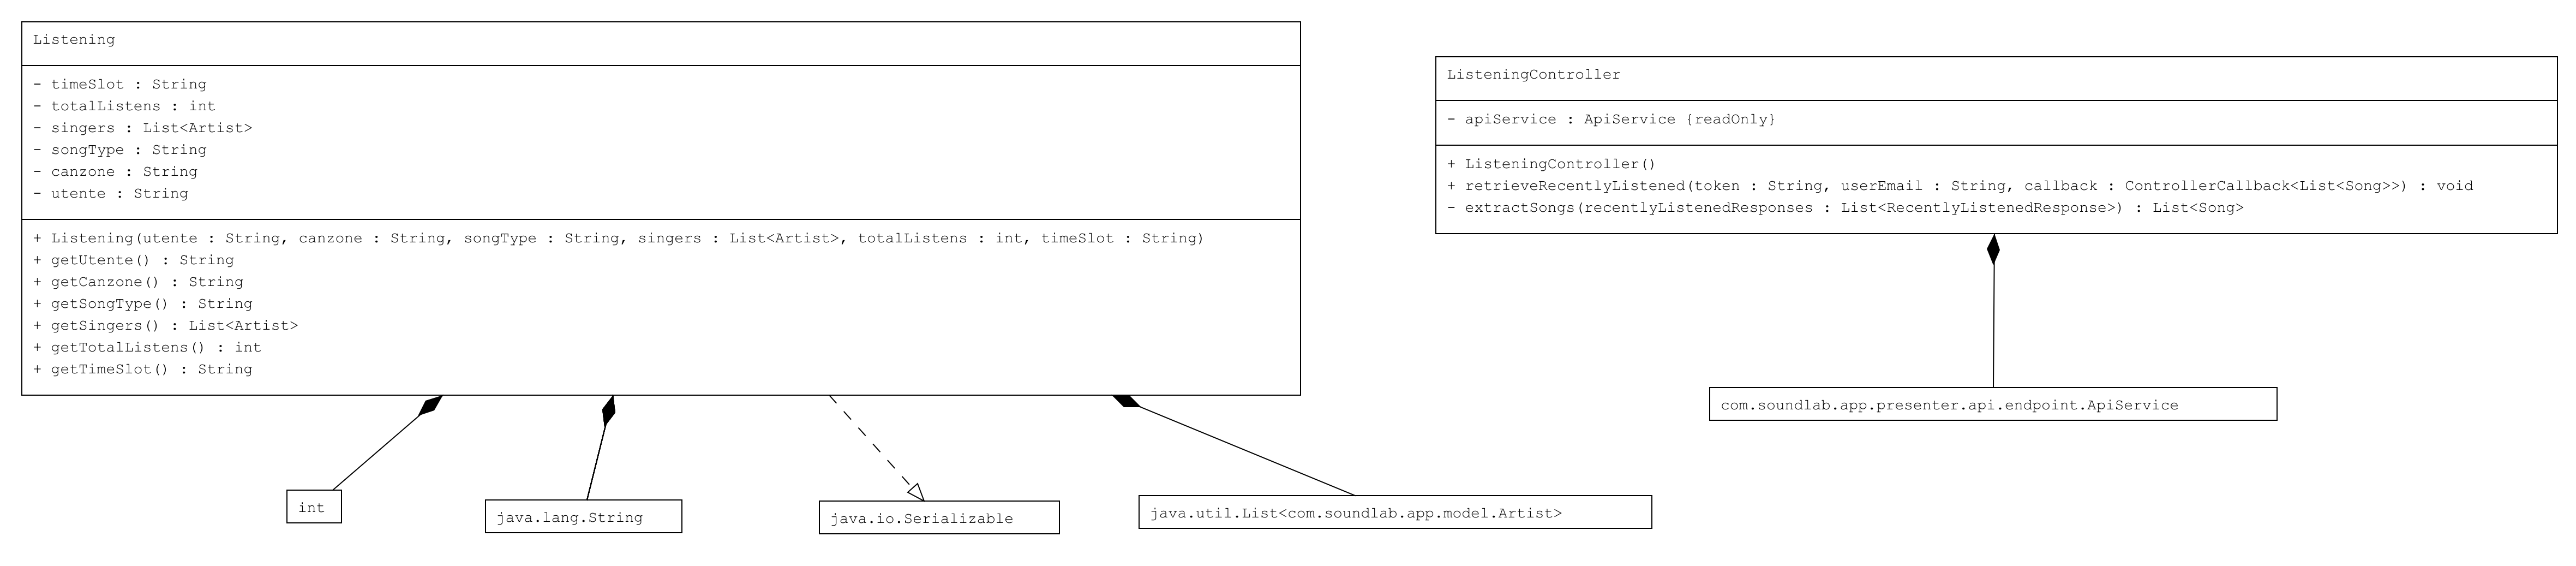
\includegraphics[width=0.9\textwidth]{Immagini/classdiagramlistening}
				\caption{Class Diagram Listening}
			\end{figure}
			\vspace{0.9cm}
			\begin{figure}[H]
				\centering
				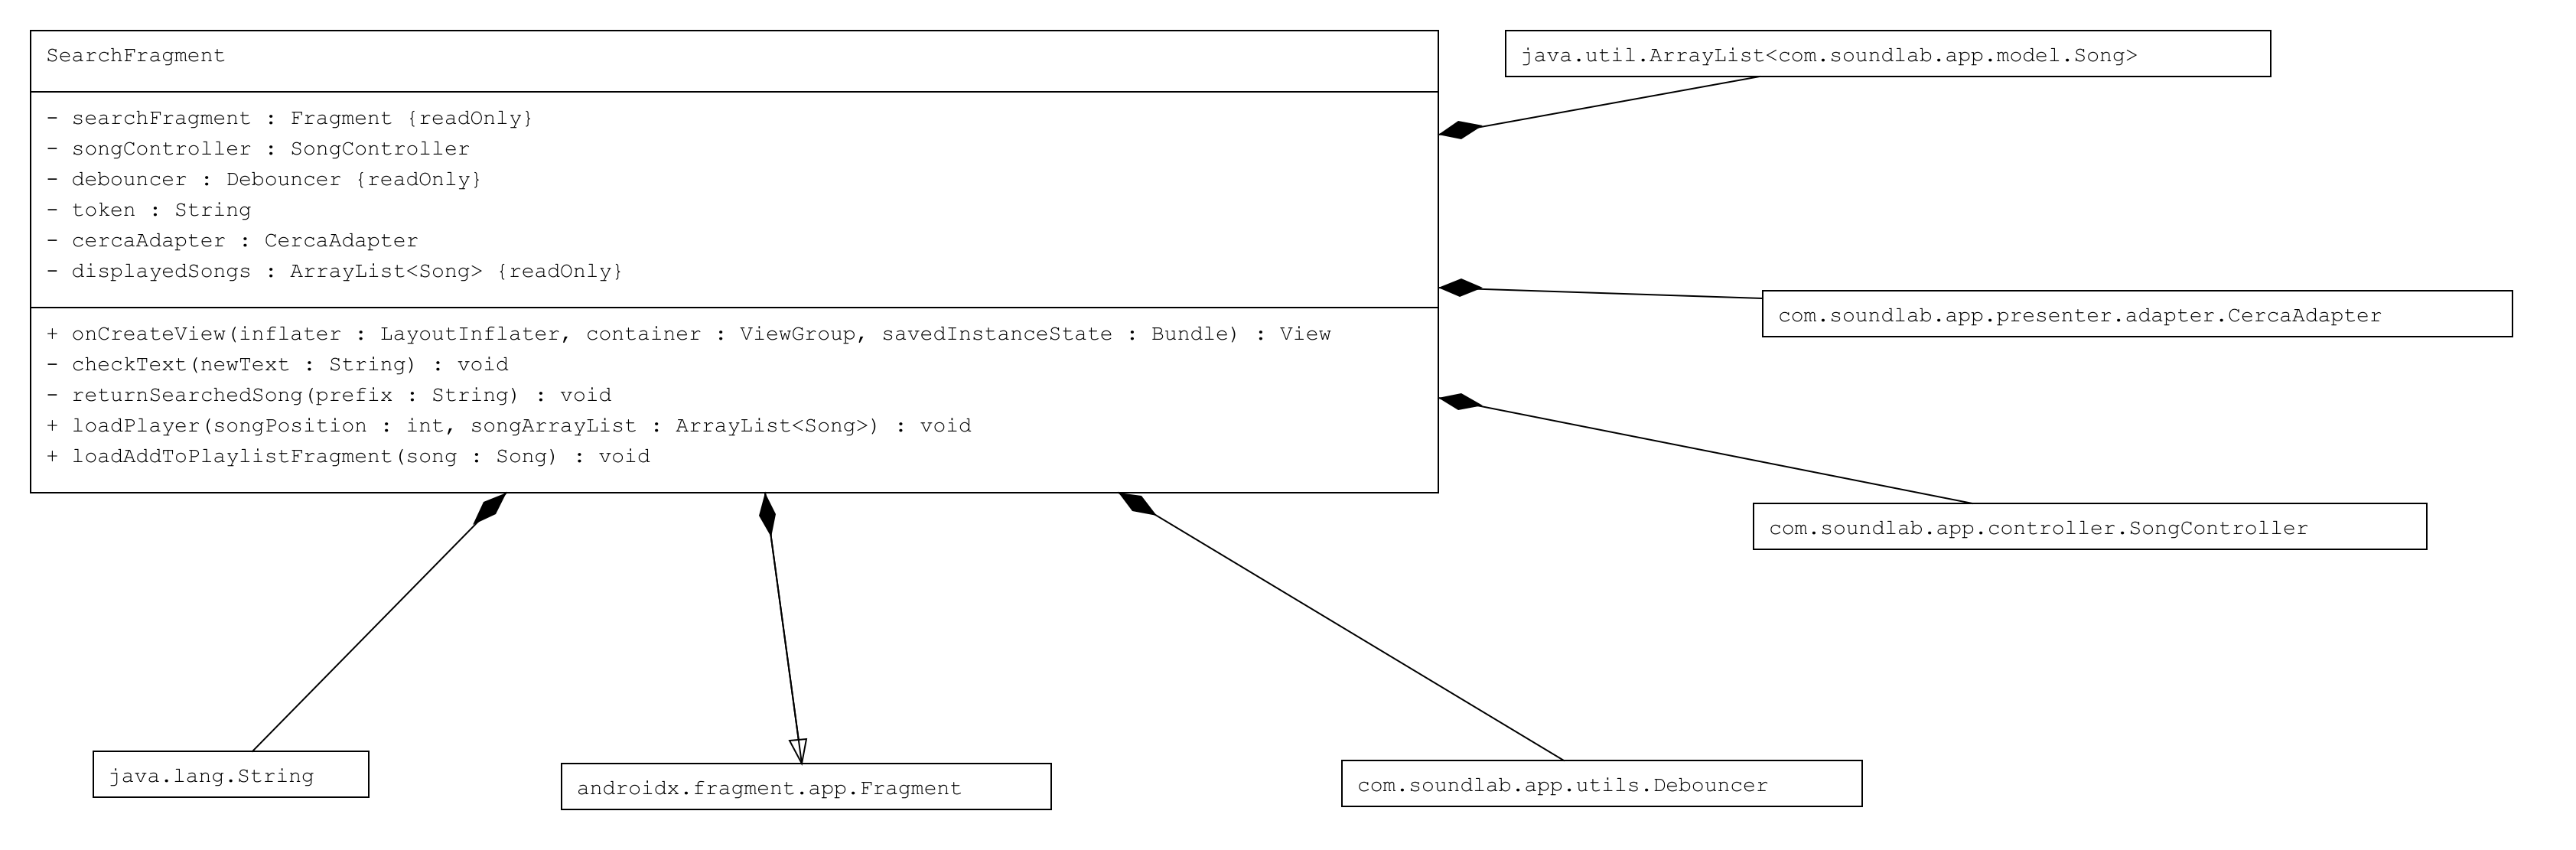
\includegraphics[width=0.9\textwidth]{Immagini/classdiagramsearch}
				\caption{Class Diagram Search}
			\end{figure}
		\subsection{Sequence diagram}
		Un \textbf{Sequence Diagram} è un diagramma previsto dall'UML utilizzato per descrivere uno \textbf{scenario}. \\Uno scenario è una determinata sequenza di azioni in cui tutte le scelte sono state già effettuate.
			\subsubsection{Sequence Diagram Aggiungi playlist}
			\begin{figure}[H]
				\centering
				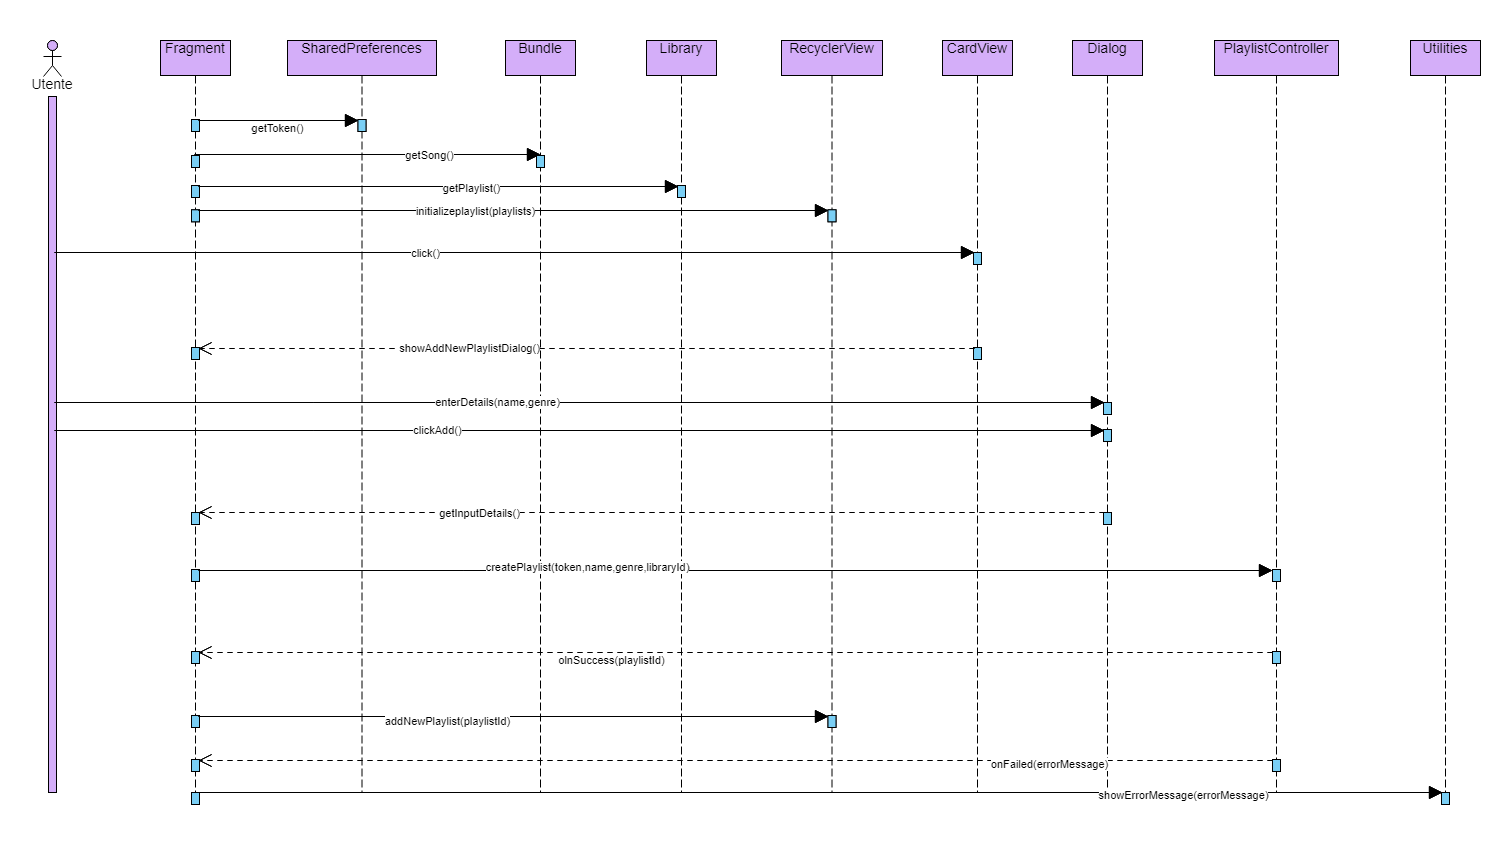
\includegraphics[width=0.9\textwidth]{Immagini/sequencediagramaggiungi}
				\caption{Class Diagram Aggiungi playlist}
			\end{figure}
			\subsubsection{Sequence Diagram Elimina profilo}
			\begin{figure}[H]
				\centering
				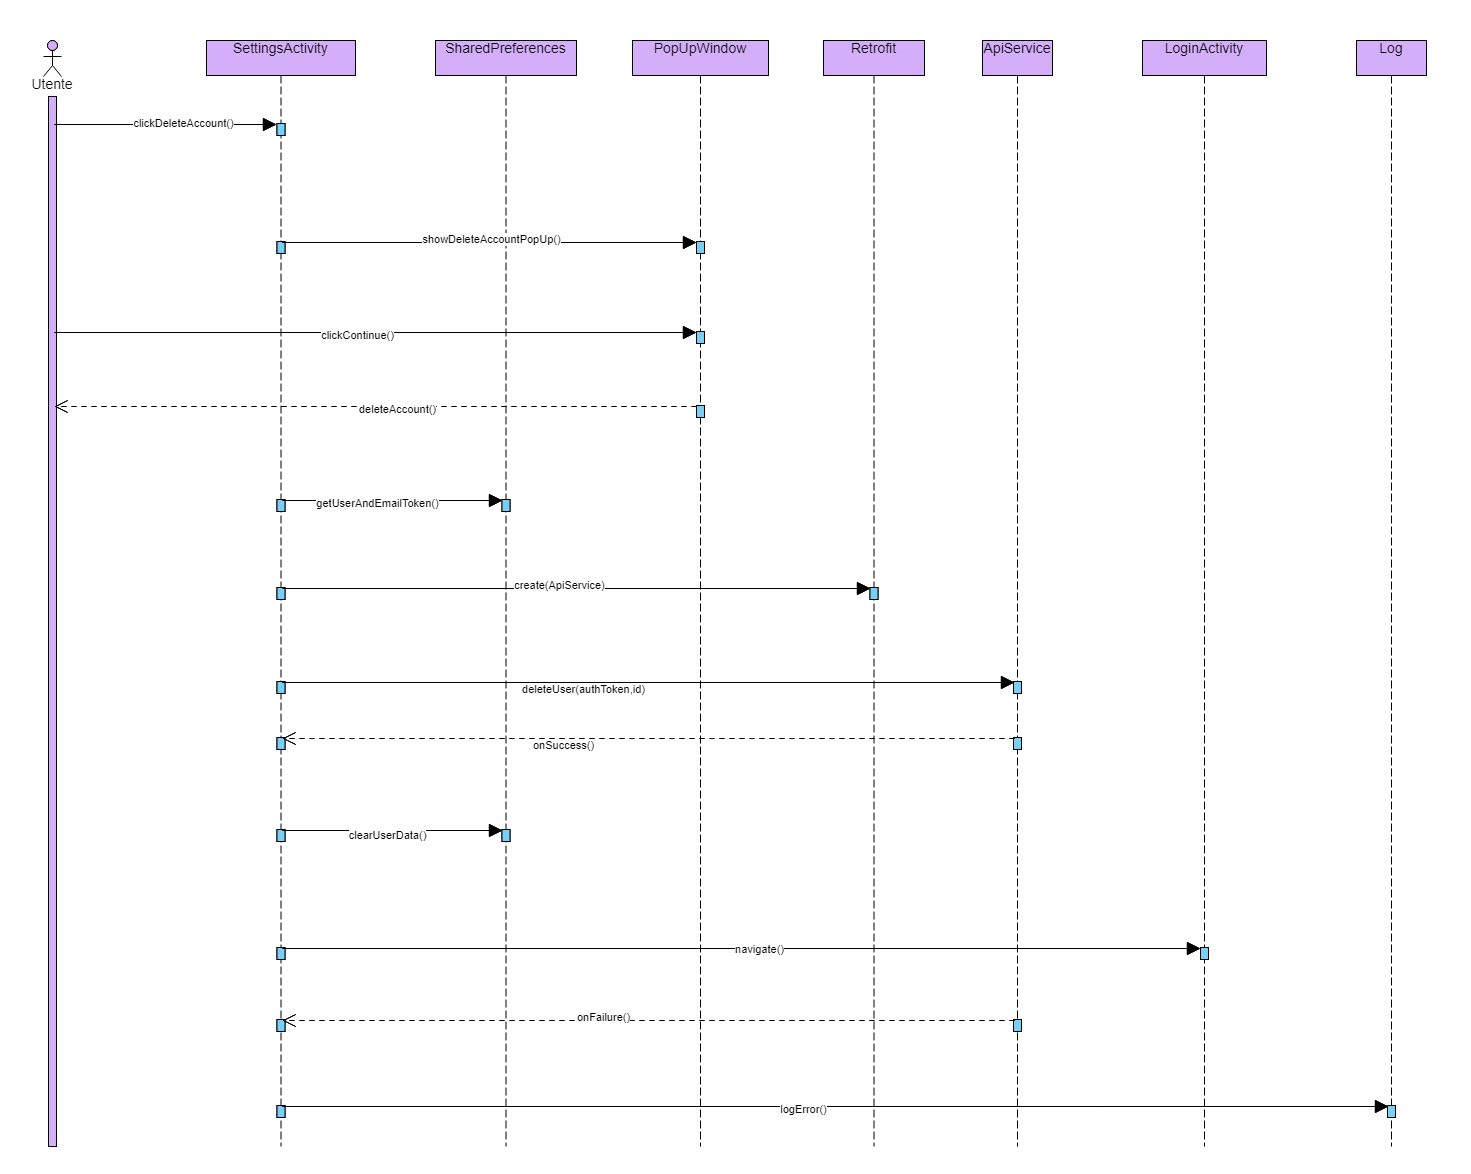
\includegraphics[width=0.9\textwidth]{Immagini/sequencediagramcancella}
				\caption{Class Diagram Elimina Profilo}
			\end{figure}
		\subsection{Activity diagram}
		Il \textbf{diagramma di attività} è un tipo di diagramma che permette di descrivere un processo attraverso dei grafi in cui i nodi rappresentano le attività e gli archi l'ordine con cui vengono eseguite.
			\subsubsection{Activity diagram}
			\begin{figure}[H]
				\centering
				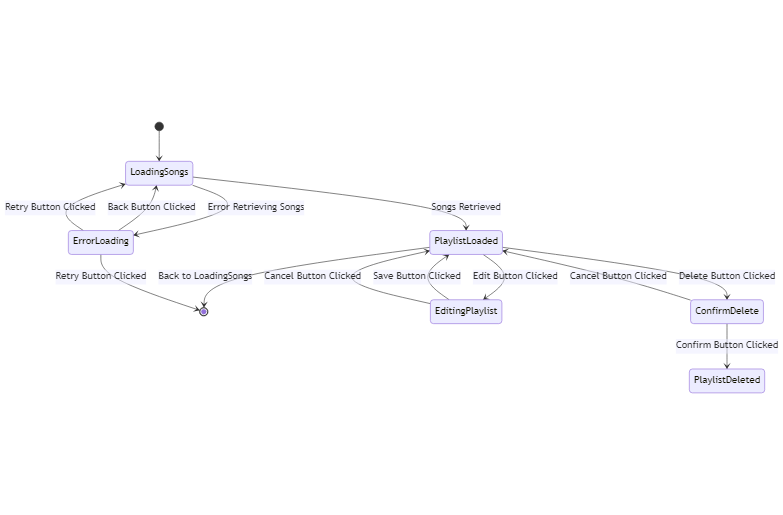
\includegraphics[width=0.9\textwidth]{Immagini/activitydiagramplaylist}
				\caption{Activity Diagram funzioni playlist}
			\end{figure}
			\vspace{0.9cm}
			\begin{figure}[H]
				\centering
				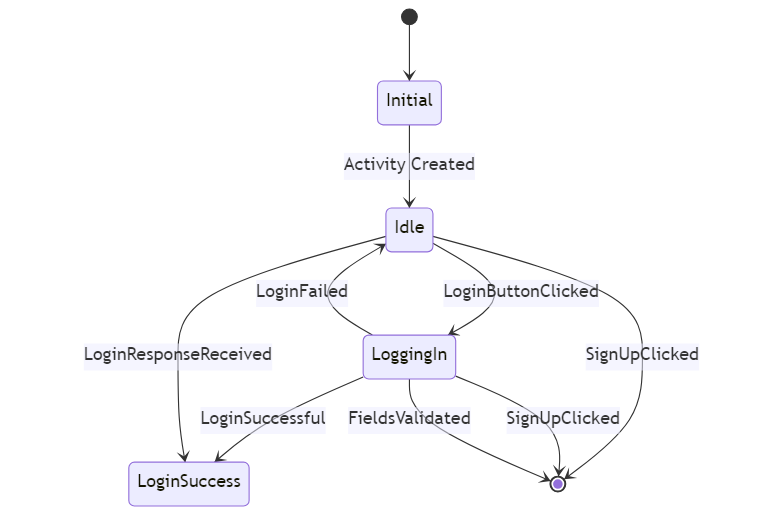
\includegraphics[width=0.9\textwidth]{Immagini/activitydiagramlogin}
				\caption{Activity Diagram Login}
			\end{figure}
			\vspace{0.9cm}
			\begin{figure}[H]
				\centering
				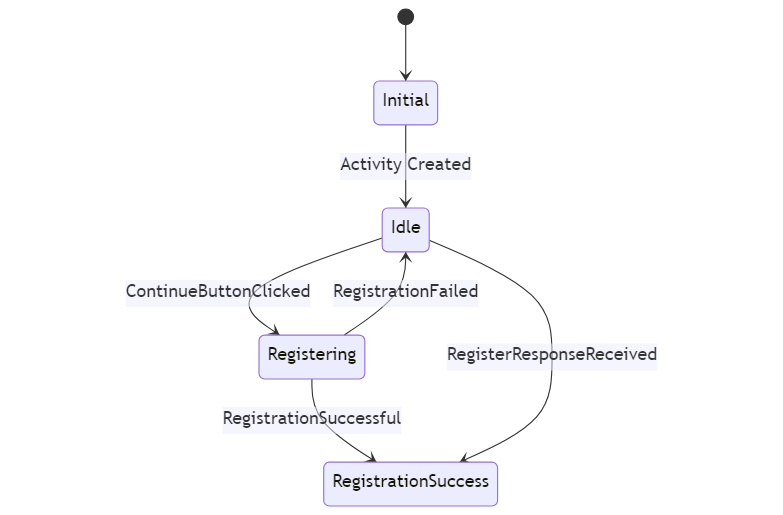
\includegraphics[width=0.9\textwidth]{Immagini/activitydiagramregistration}
				\caption{Activity Diagram Registrazione}
			\end{figure}
			\vspace{0.9cm}
			\begin{figure}[H]
				\centering
				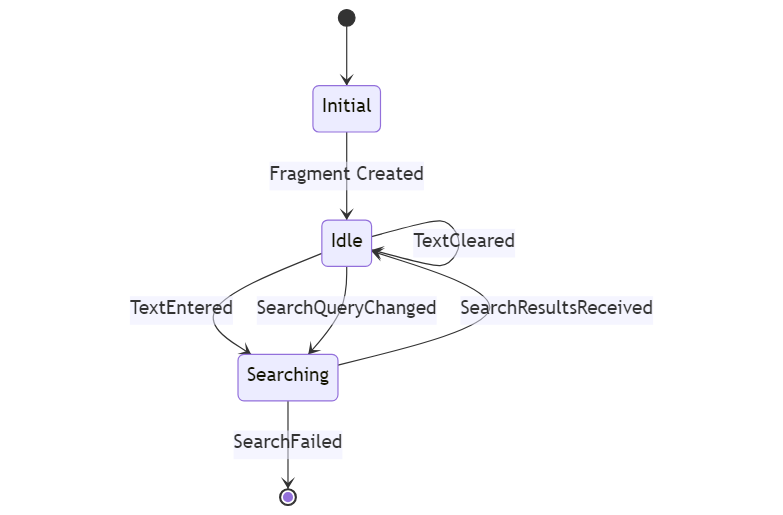
\includegraphics[width=0.9\textwidth]{Immagini/activitydiagramsearch}
				\caption{Activity Diagram Ricerca}
			\end{figure}
			\vspace{0.9cm}
			\begin{figure}[H]
				\centering
				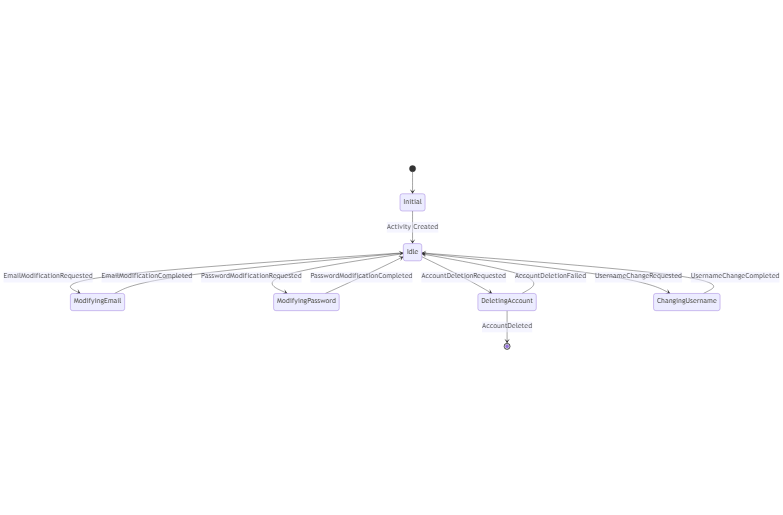
\includegraphics[width=1.0\textwidth]{Immagini/activitydiagramsettings}
				\caption{Activity Diagram azioni settings}
			\end{figure}
			\newpage
			
	\section{Design di sistema}
		\subsection{Analisi architetturale}
		L'architettura usata per questo progetto comprende un insieme di soluzioni e strategie di famosi \textbf{design pattern}.
		\\
		In particolare, in questa sezione del documento, verrà analizzata l'\textbf{architettura client-server} utilizzata.
		\\
		Con la parola \textit{client}, indichiamo i dispositivi android mobile mentre con la parola \textit{server}, indichiamo il backend utilizzato per gestire i servizi offerti ai clienti dal nostro applicativo.
		\begin{figure}[H]
			\centering
			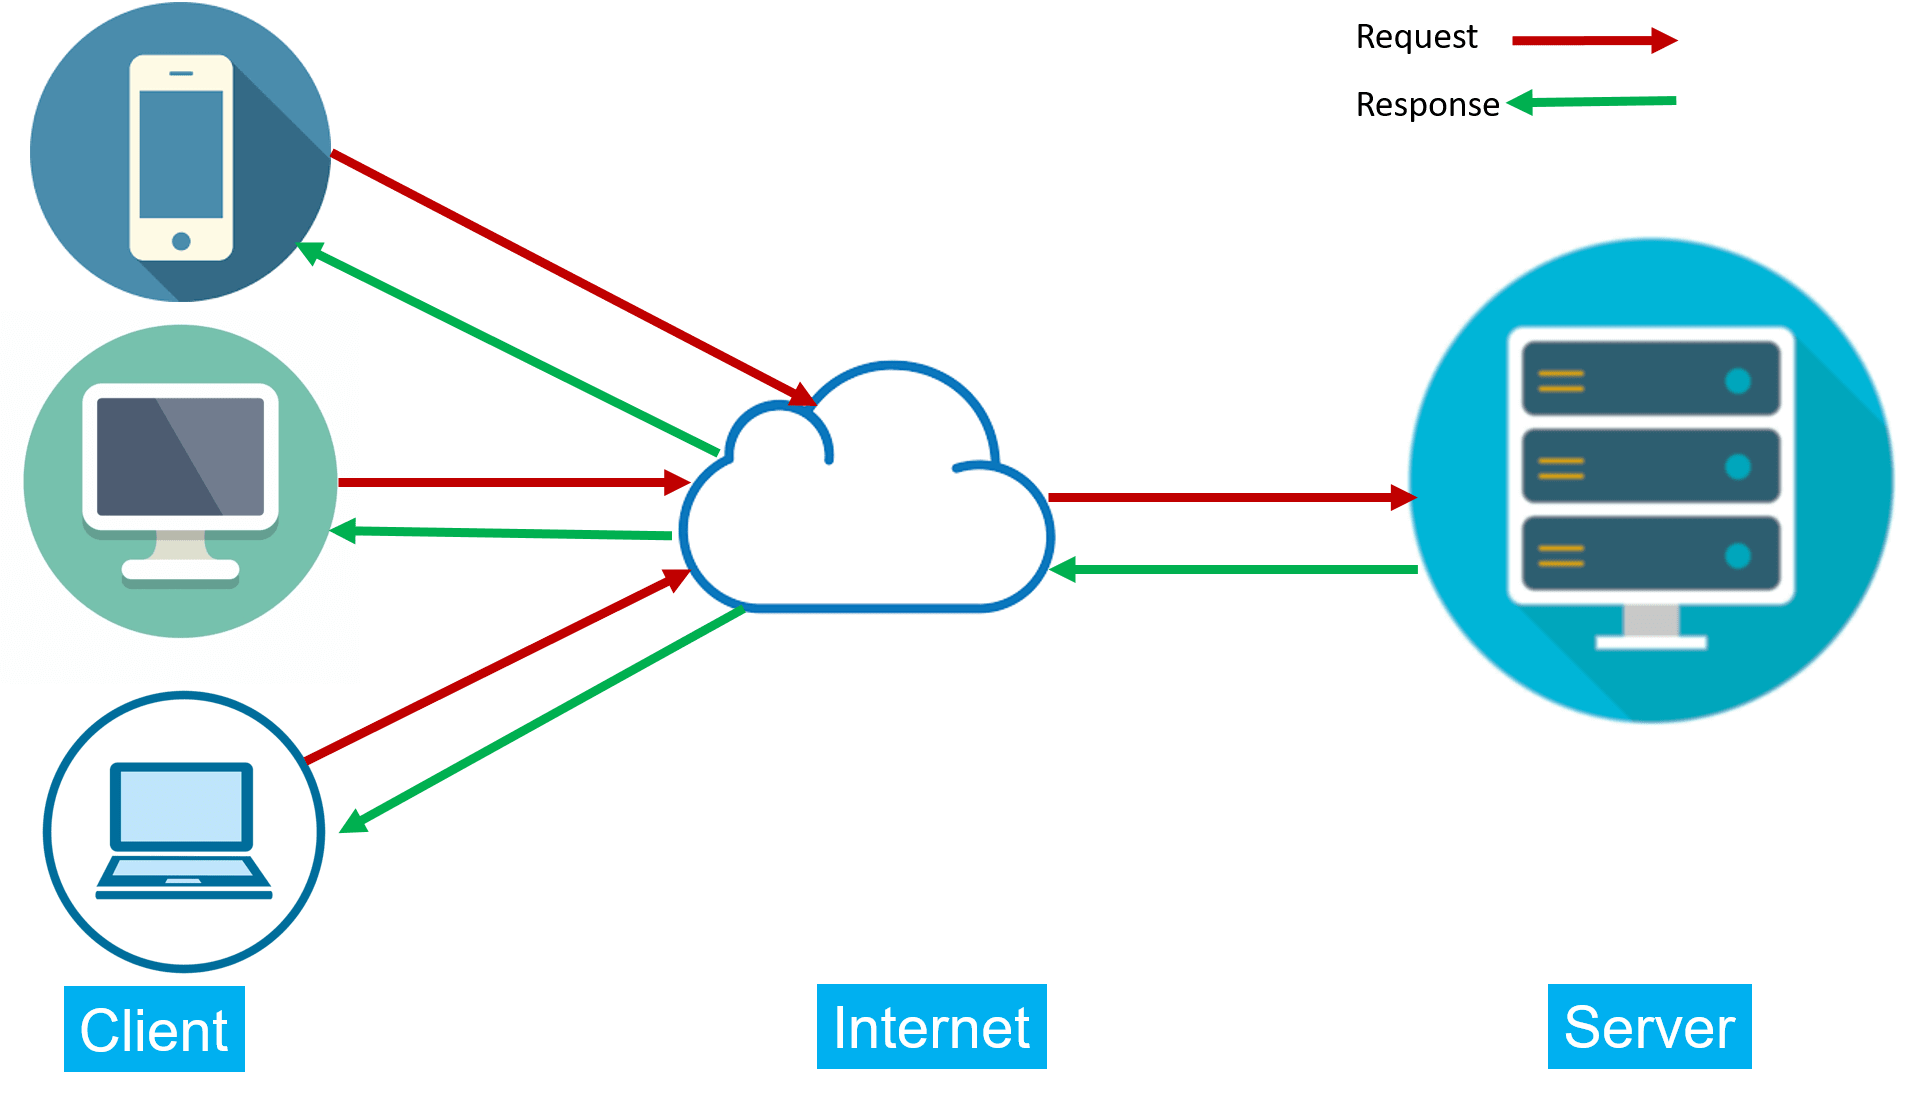
\includegraphics[width=0.9\textwidth]{Immagini/model}
			\caption{Client-server model}
		\end{figure}
		\subsubsection{Descrizione architettura cloud}
		SoundLab offre un back-end con le seguenti caratteristiche:
		\begin{itemize}
			\item \textbf{\textit{\textcolor{dark_purple}{Elasticità}}}
			\item \textbf{\textit{\textcolor{dark_purple}{Scalabilità}}}
			\item \textbf{\textit{\textcolor{dark_purple}{Economicità}}}
			\item \textbf{\textit{\textcolor{dark_purple}{Astrazione}}}
			\item \textbf{\textit{\textcolor{dark_purple}{Sicurezza}}}
			\item \textbf{\textit{\textcolor{dark_purple}{Virtualizzazione}}}
		\end{itemize}
		Tali servizi sono stati offerti grazie all'utilizzo dei \textbf{servizi on demand in Cloud di AWS}\footnote{\textit{Amazon Web Services, Inc.} è una sussidiaria di Amazon, che fornisce servizi di cloud computing su un'omonima piattaforma on demand}, applicando la seguente architettura:
		\begin{figure}[H]
			\centering
			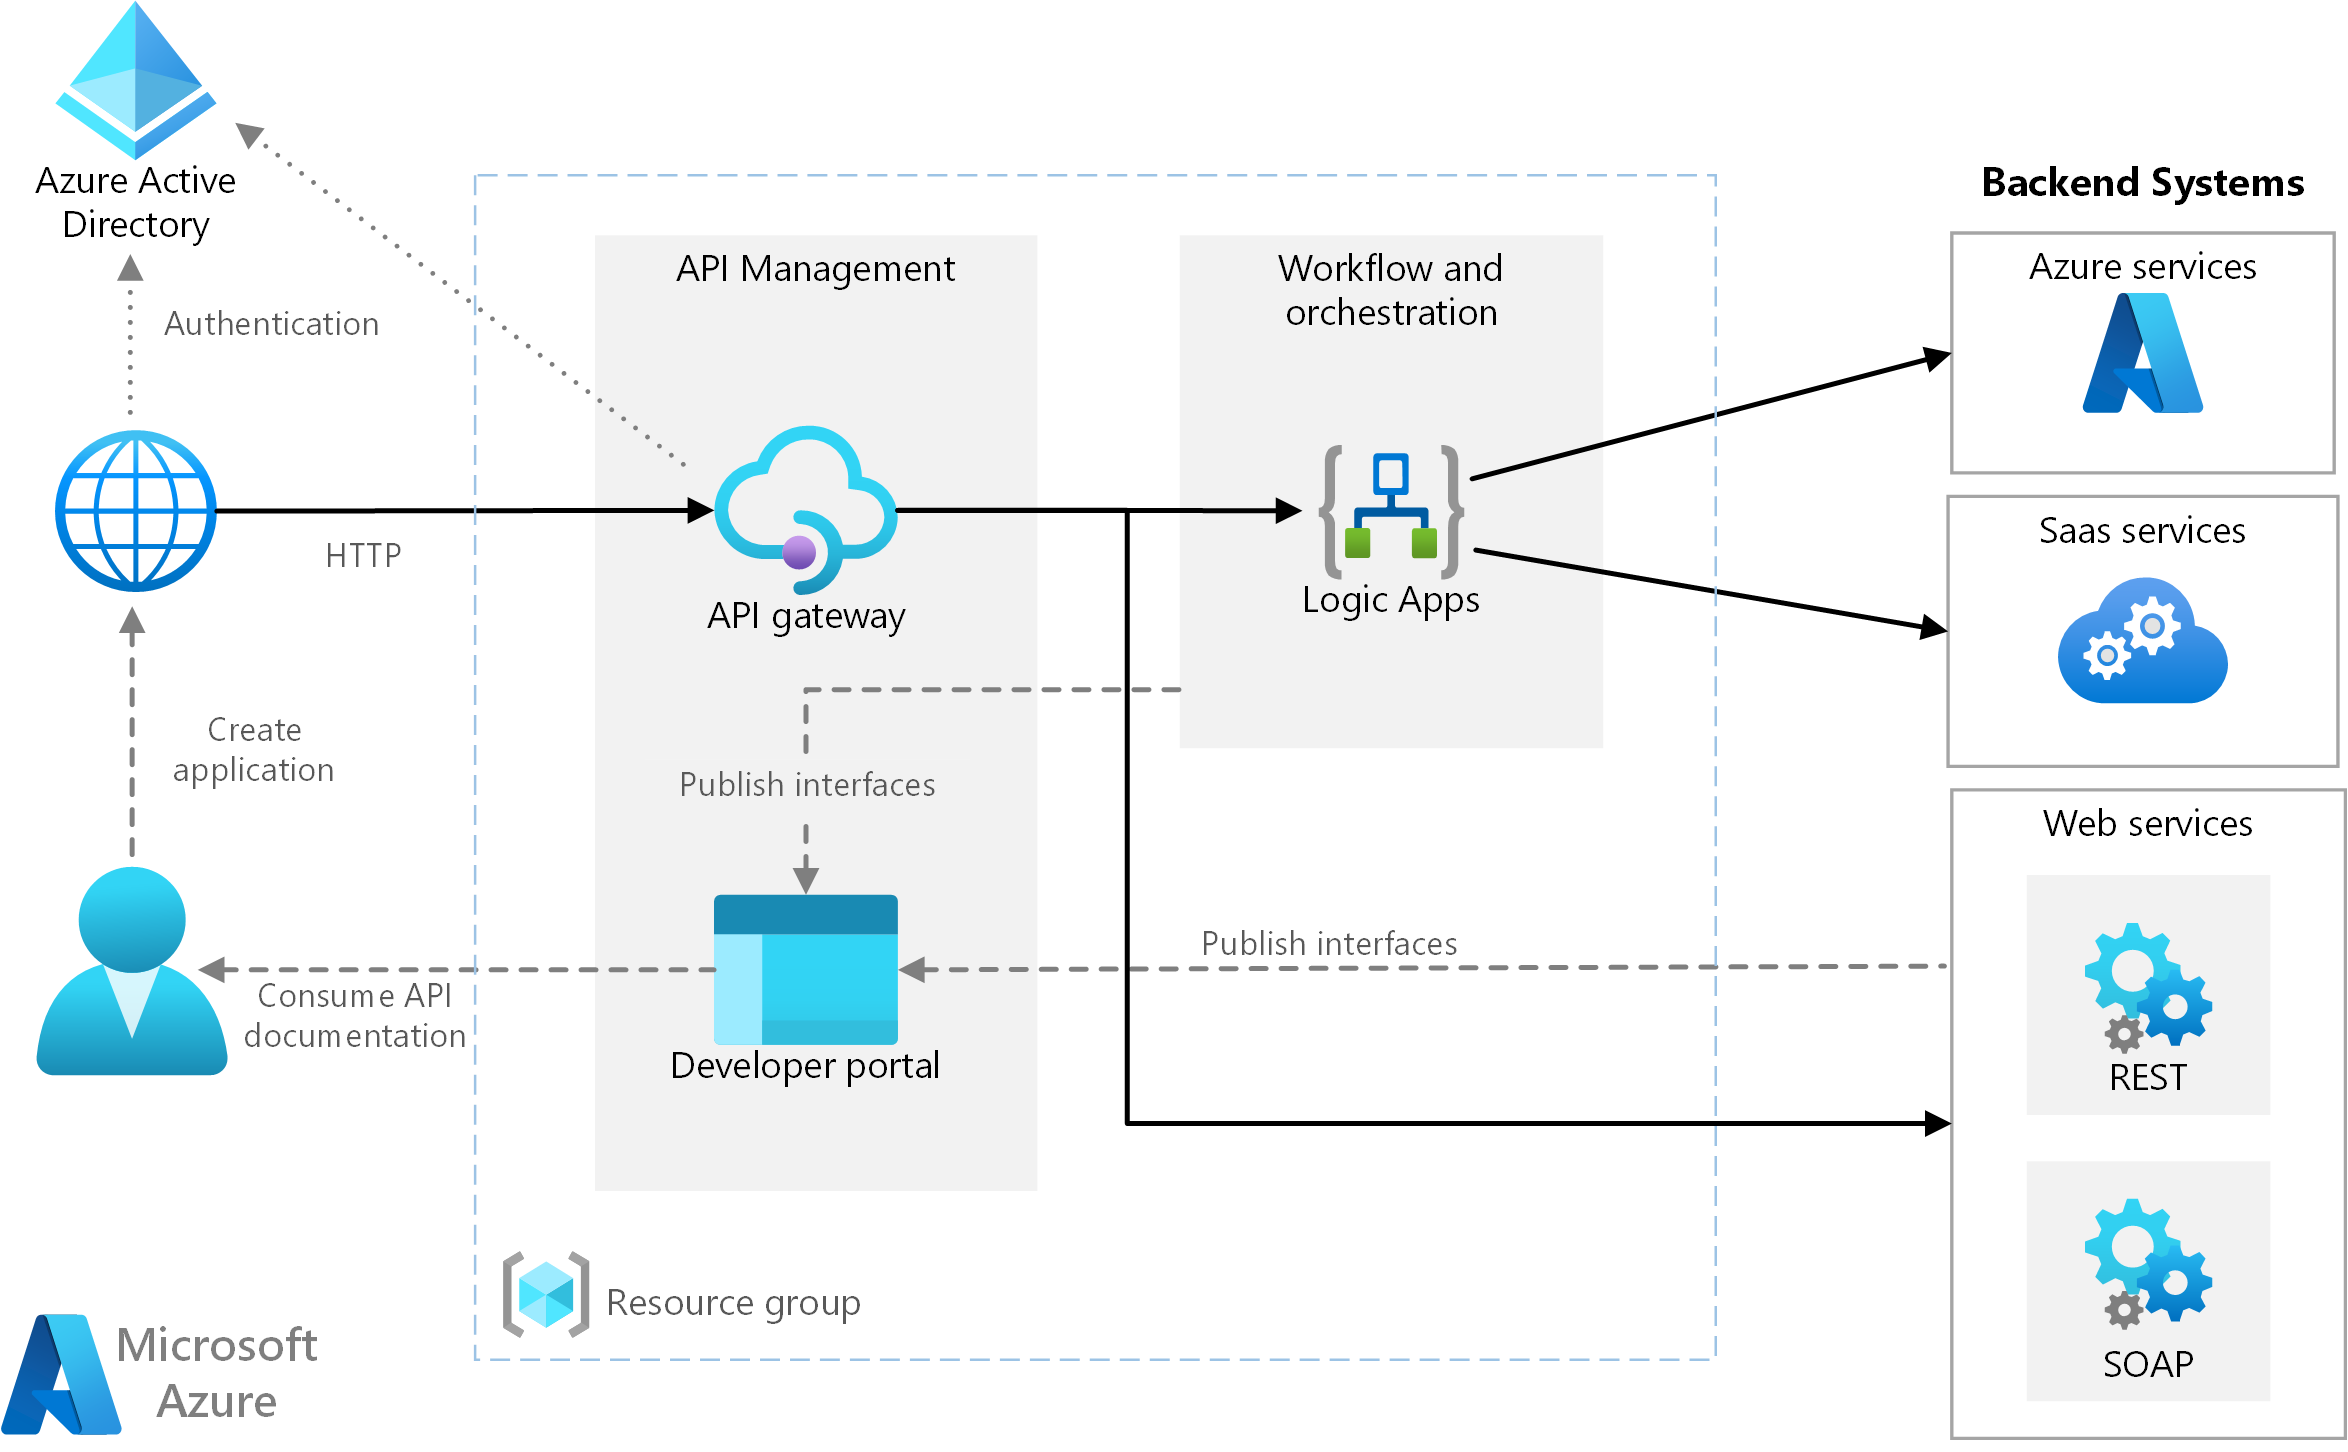
\includegraphics[width=0.9\textwidth]{Immagini/springboot}
			\caption{Architettura di sistema}
		\end{figure}
		Le tecnologie adoperate sono:
		\begin{itemize}
			\item \textbf{\textit{\textcolor{dark_purple}{Springboot}}} che risulta essere un tassello importantissimo per il backend. Questo famosissimo framework di Java offre l'opportunità di creare un proprio insieme personalizzato di \textbf{route di REST API} personalizzate. Inoltre, SpringBoot è il diretto connesso al server Database tramite operazioni \textbf{CRUD}.
			\item \textbf{\textit{\textcolor{dark_purple}{Amazon AWS-RDS}}} che è un sistema che semplifica l’impostazione, il funzionamento e il dimensionamento di database relazionali nel cloud.Questo servizio fornisce una capacità ridimensionabile efficiente nei costi,automatizzando al tempo stesso le attività di amministrazione più dispendiose in termini di tempo.
			\item \textbf{\textit{\textcolor{dark_purple}{Amazon AWS-S3}}} che è un servizio di archiviazione di oggetti che offre scalabilità, disponibilità dei dati,sicurezza e prestazioni all’avanguardia nel settore. I clienti di tutte le entità e settori possono archiviare e proteggere qualsiasi quantità di dati per qualsiasi caso d’uso. Con classi di archiviazione convenienti e caratteristiche di gestione di facile utilizzo, è possibile ottimizzare i costi, organizzare i dati e configurare controlli di accesso ottimizzati per soddisfare specifici requisiti aziendali,organizzativi e di conformità.
			\item \textbf{\textit{\textcolor{dark_purple}{Amazon AWS-Amplify}}} che consiste in un set di strumenti e caratteristiche appositamente progettati per consentire agli sviluppatori front-end di applicazioni Web e per dispositivi mobili di costruire rapidamente e facilmente applicazioni full-stack in AWS,con la flessibilità di sfruttare i vari servizi AWS man mano che i casi d’uso si evolvono. Con Amplify, è possibile configurare un back-end per app Web oper dispositivi mobili, connettere l'app in pochi minuti, costruire visivamente un’interfaccia utente front-end Web e gestire facilmente i contenuti dell’app al di fuori della console AWS
		\end{itemize}
		
		\subsubsection{Il server}
		Il server è scritto interamente in \textbf{Springboot}.
		Si tratta di un framework open source di livello aziendale molto diffuso per la creazione di applicazioni autonome, adatte ad ambienti di produzione che vengono eseguite su \textbf{JVM (Java Virtual Machine)}.\\
		Per una buona gestione e per facilitare tante qualità quali il riutilizzo di codice, dependency injection e altro abbiamo optato per un famoso \textbf{DesignPattern}, ovvero \textbf{MVC}.
		\begin{figure}[H]
			\centering
			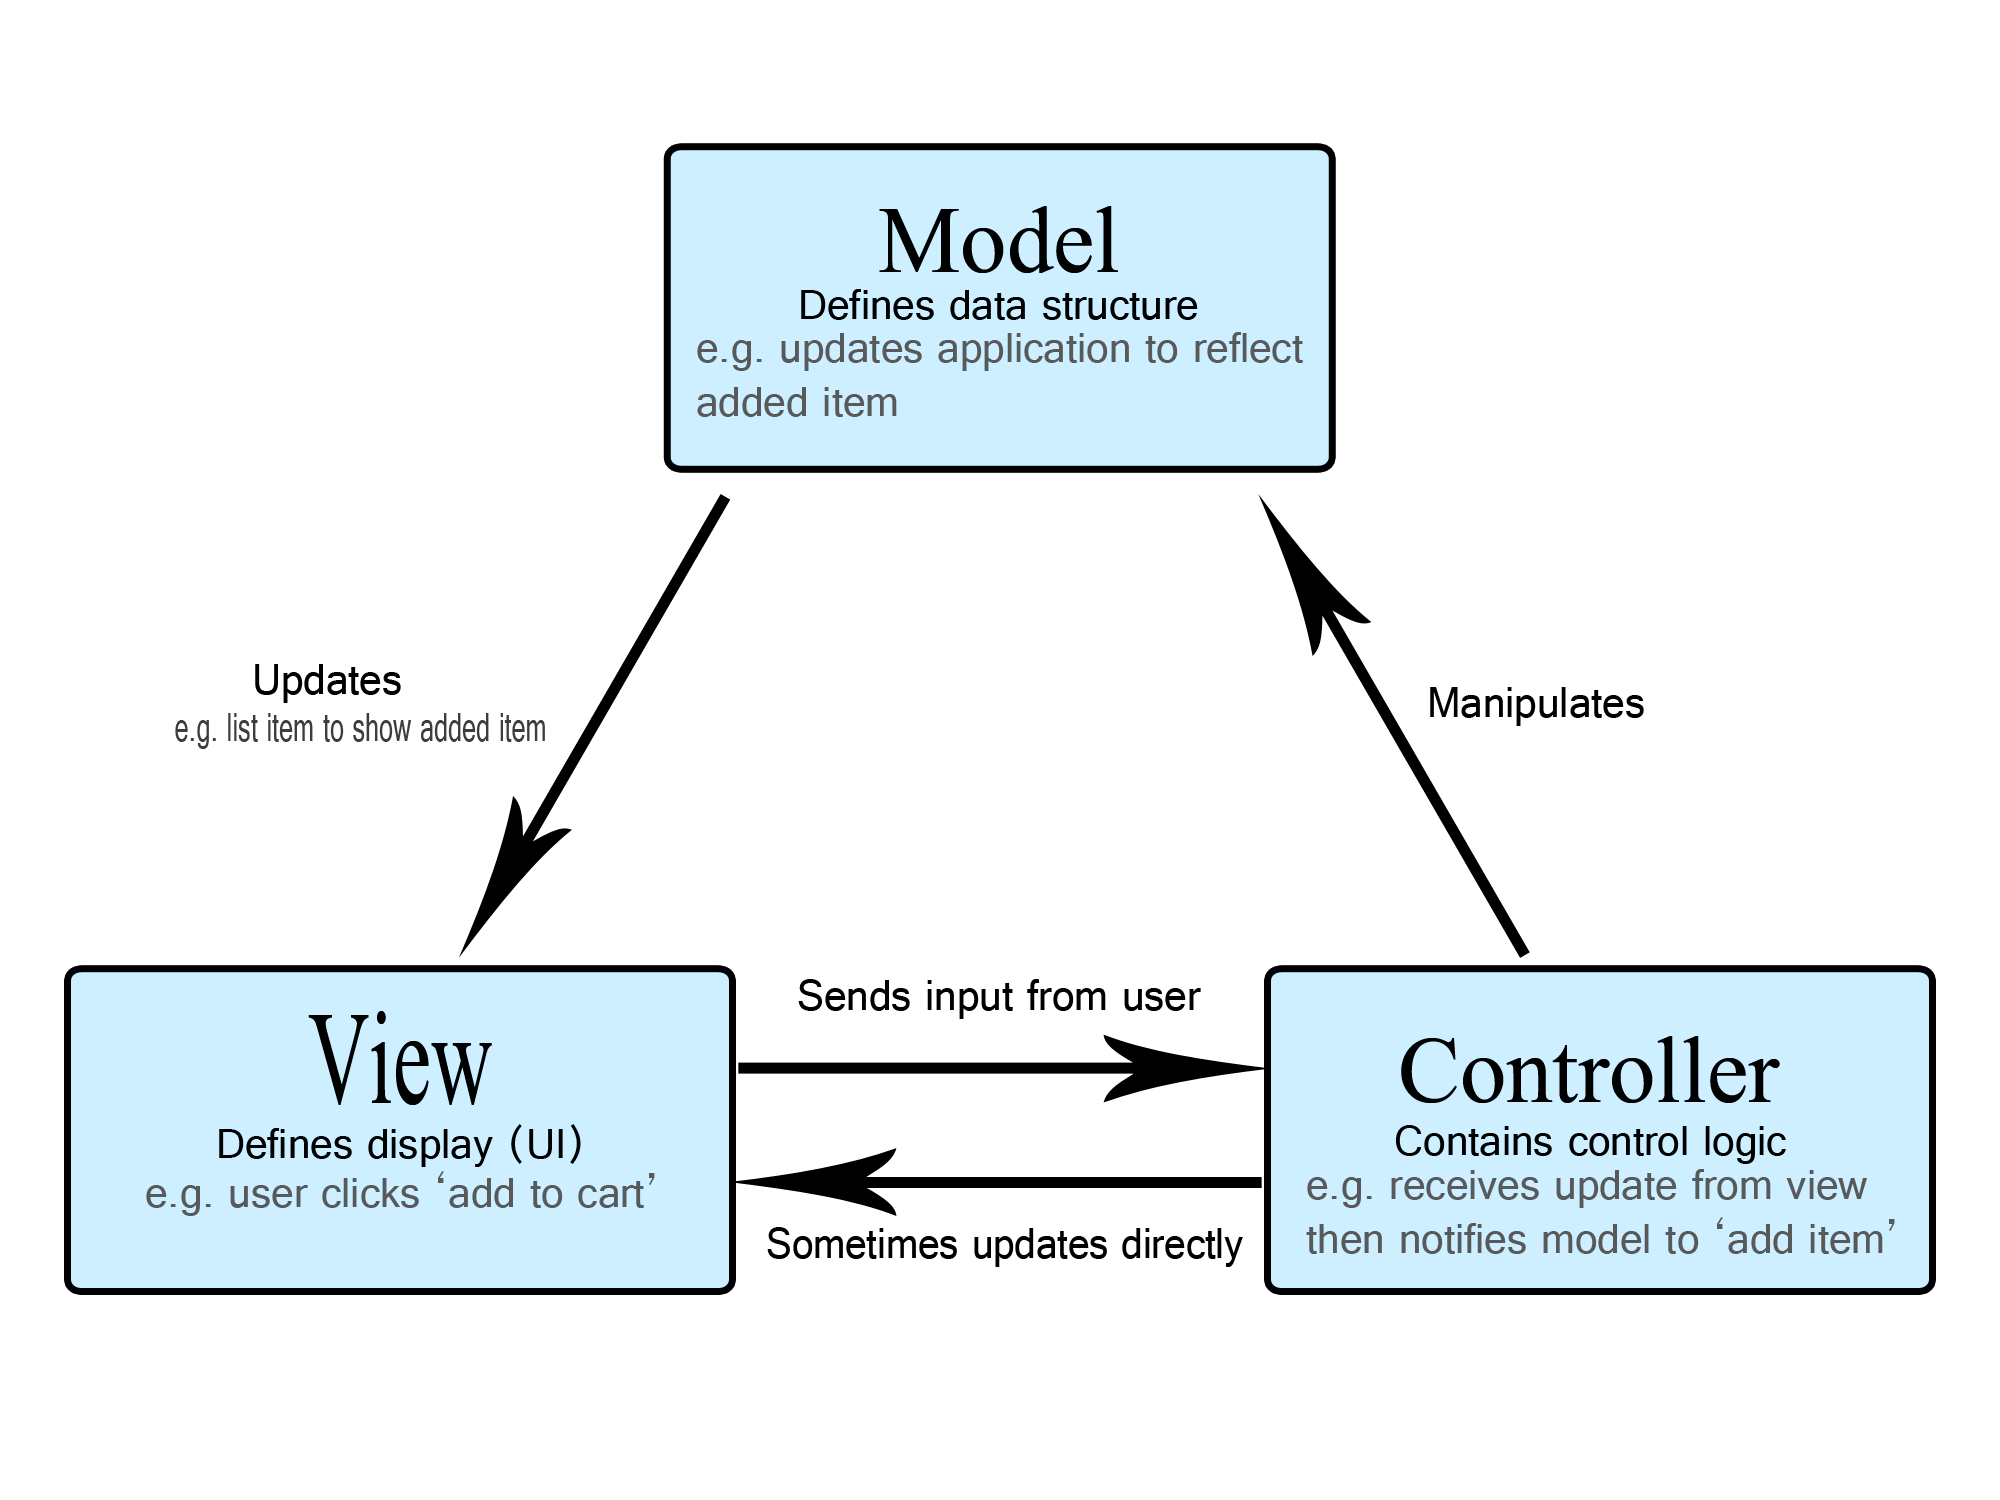
\includegraphics[width=0.9\textwidth]{Immagini/mvc}
			\caption{Design Pattern MVC}
		\end{figure}
		Il design pattern segue delle linee guida per SpringBoot, infatti sono stati individuati i seguenti componenti:
		\begin{itemize}
			\item \textbf{Components:} componenti del backend quali contorller, service, repository (tutte sottoclassi)
			\item \textbf{Model:} oggetti che rappresentato una figura concreta che mappata viene per essere entità di un database
			\item \textbf{Model DTO:} \textit{Data Transfer Object} sono il mezzo di comunicazione entrante/uscente del server
			\item \textbf{Controller:} gestiscono i metodi da HTTP (GET, POST, PUT, DELETE) e relative rotte e sotto-rotte
			\item \textbf{Service:} layer soggetto a dependency injection molto importante e intermediario tra repository e controller
			\item \textbf{Repository:} diretta comunicazione con la logica di database sottostante, attraverso JPA e altri moduli si interfacciano con interfacce per fare
			operazioni CRUD
		\end{itemize}
	Nel prossimo paragrafo elencheremo le \textbf{REST API} create appositamente per offrire i servizi tramite \textbf{Springboot} per i clienti di SoundLab.
		\subsubsection{Rest Api}
		Il protocollo di comunicazione è quello \textbf{HTTP}.
		\begin{itemize}
			\item \textbf{POST:} Il metodo POST viene utilizzato per inviare dati al server per creare o aggiornare risorse. Quando si effettua una richiesta POST, i dati vengono solitamente inviati nel corpo della richiesta. Questo metodo è comunemente utilizzato per inviare i dati di un modulo HTML ad un server o per creare nuove risorse tramite un'API.
			\item \textbf{GET:} Il metodo GET viene utilizzato per richiedere dati dal server. Quando si effettua una richiesta GET, i parametri e i dati della richiesta sono inclusi nell'URL. Questo metodo è comunemente utilizzato per ottenere risorse esistenti dal server o per recuperare dati da un'API.
			\item \textbf{DELETE:} Il metodo DELETE viene utilizzato per eliminare una risorsa specifica dal server. Quando si effettua una richiesta DELETE, l'identificatore della risorsa da eliminare è solitamente incluso nell'URL o nel corpo della richiesta. Questo metodo è comunemente utilizzato per cancellare risorse esistenti tramite un'API.
		\end{itemize}
		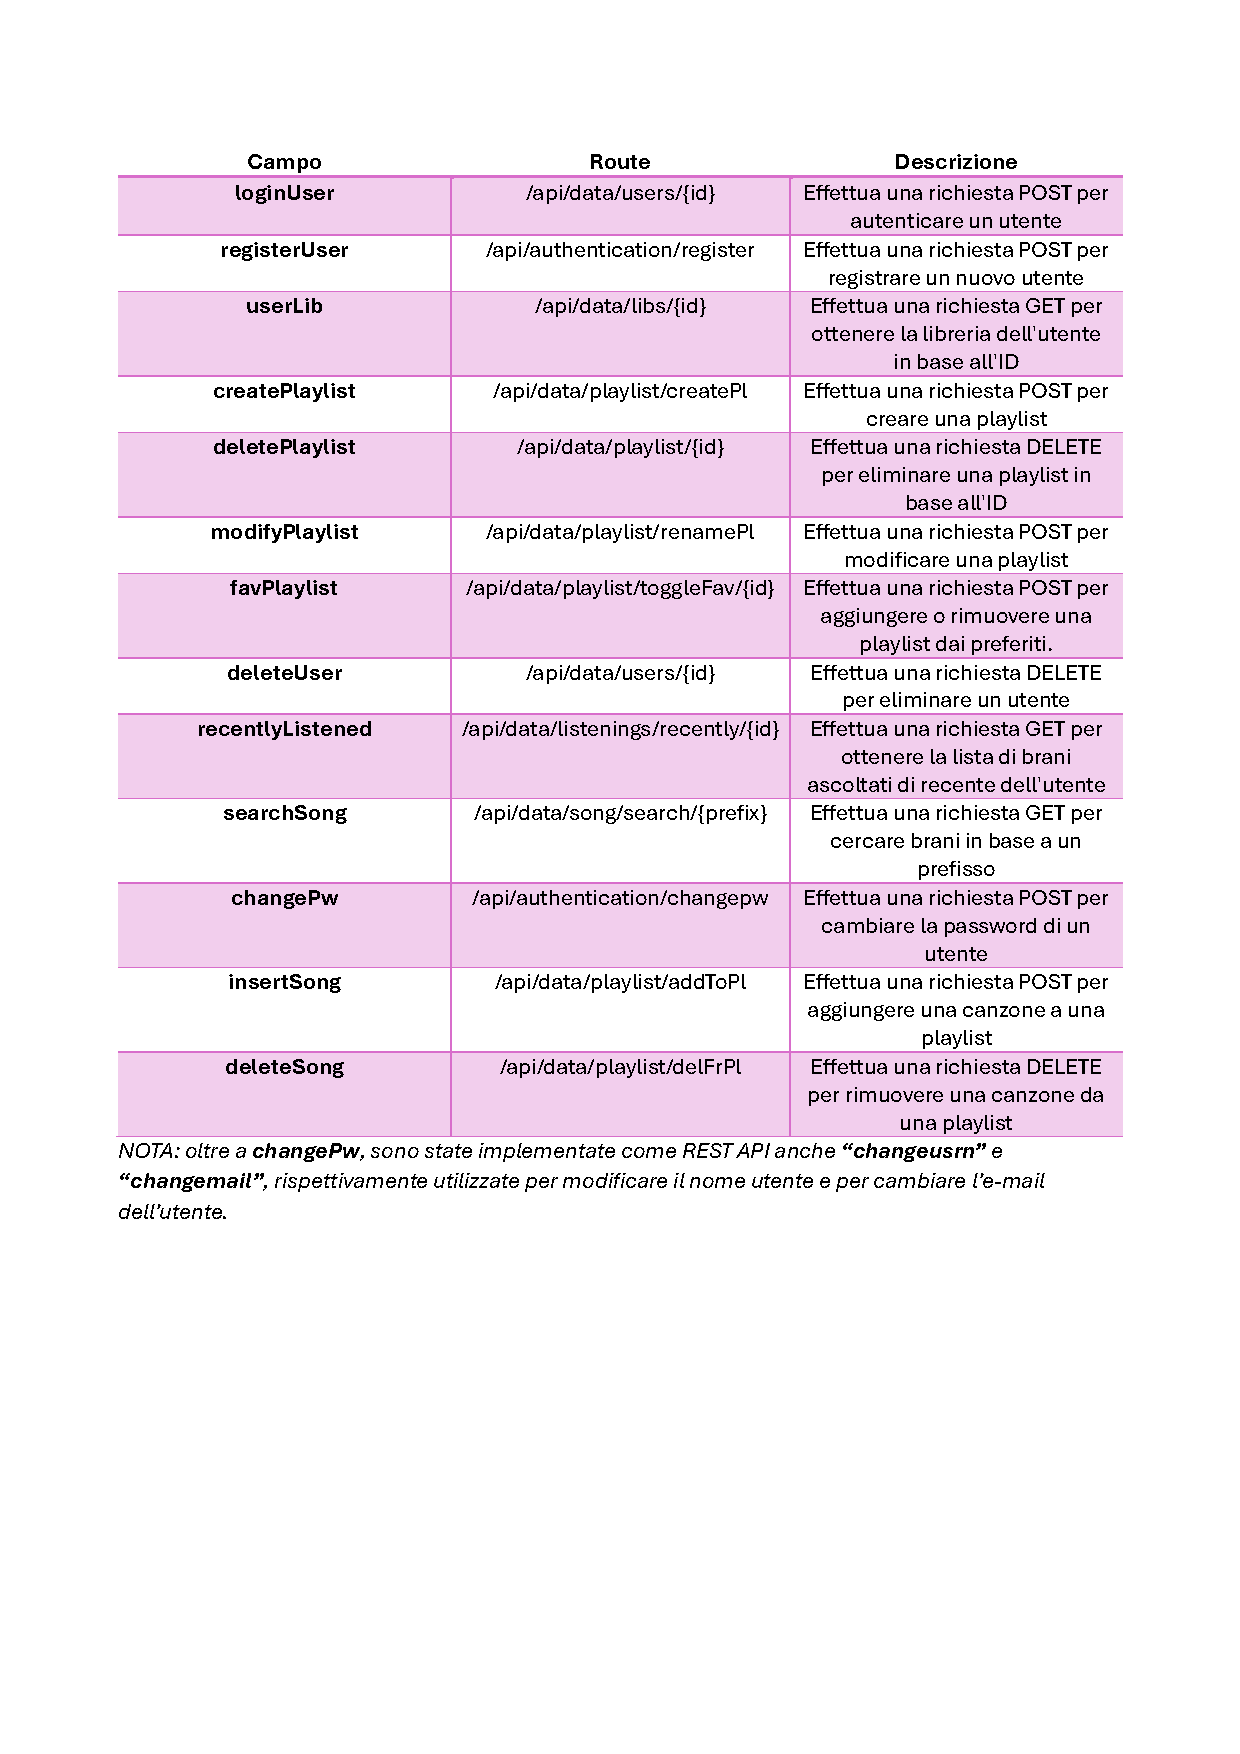
\includepdf[pages={1}]{Documenti/restapi.pdf}
		\subsubsection{Il client}
		Il client di SoundLab è stato sviluppato su piattaforma \textbf{Android}. I vantaggi di lavorare su android sono molteplici uno tra quali l’\textbf{Open Source}, infatti grazie ad android si ha avuto la possibilità di avere accesso a numerose librerie utili al fine di sviluppare al meglio l'applicativo.
		Per il progetto abbiamo usato il design pattern \textbf{MVP}:
		\begin{itemize}
			\item \textbf{Model:} rappresenta il modello dei dati di interesse per l’applicazione.Tale livello si occupa di incapsulare lo stato dell’applicazione, gestisce l’accesso alla sorgente dei dati, fornisce funzionalità per l’aggiornamento dello stato e l’accesso ai dati. Nel client android sviluppato, è compito di questo livello gestire la comunicazione diretta con le APILambda e quindi si occupa della formattazione delle richieste e delladecodifica delle risposte. Infine, il MODEL notifica al PRESENTER il cambiamento di stato
			\item \textbf{View:} questo livello rappresenta l’interfaccia utente, permettendo l’interazione con esso e fornendo una rappresentazione grafica ed interattiva del model. La responsabilità di questo livello è la presentazione dei dati e dello stato dell’applicazione. Inoltre, esso riceve notifiche dal PRESENTER e aggiorna la visualizzazione
			\item \textbf{Presenter:} tale livello definisce la logica di controllo e le funzionalità applicative. Quindi, è compito di questo livello gestire gli eventi ed i comandi generati dall’utente: in base a questi ultimi, esso opera sul model. Infine, tale livello si occupa di selezionare/aggiornare il livello VIEW in base ai dati recuperati.
		\end{itemize}
		\begin{figure}[H]
			\centering
			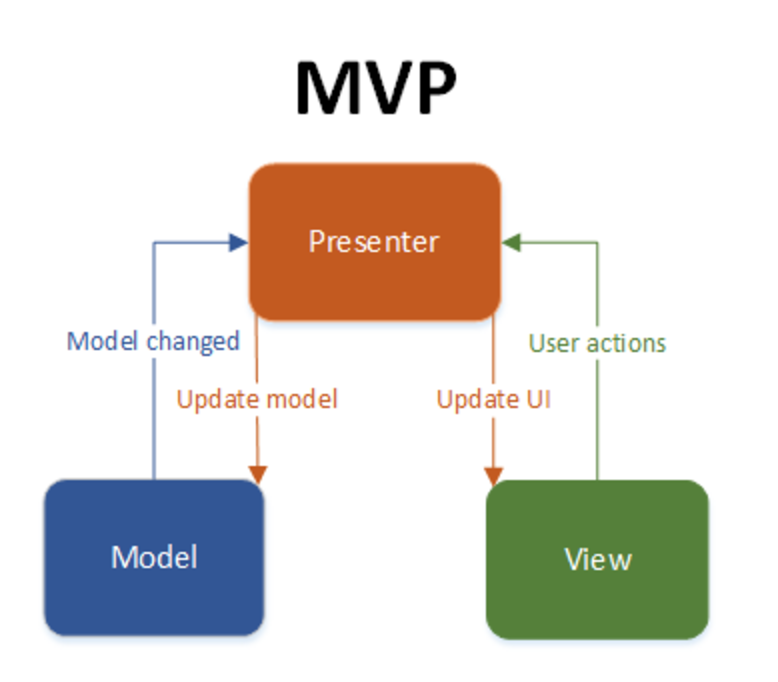
\includegraphics[width=0.9\textwidth]{Immagini/mvp}
			\caption{Design Pattern MVP}
		\end{figure}
		\newpage
		\subsubsection{Supporti}
		\textbf{Retrofit} è una libreria per Android che semplifica l'utilizzo delle API RESTful all'interno di un progetto. Fornisce un modo semplice e intuitivo per definire le richieste HTTP, gestire le risposte del server e convertire automaticamente i dati JSON in oggetti Java.
		\begin{itemize}
			\item \textbf{Interfacce API:} In Retrofit, si definiscono le API RESTful come interfacce Java. Ogni metodo dell'interfaccia rappresenta un'operazione su una risorsa del server e specifica il tipo di richiesta HTTP (GET, POST, DELETE, ecc.), l'URL relativo e i parametri richiesti. Si possono anche specificare gli header di autenticazione o il corpo della richiesta utilizzando annotazioni specifiche di Retrofit.
			\item \textbf{Client Retrofit:} Si può creare un'istanza di Retrofit utilizzando il Retrofit.Builder e configurarlo con l'URL di base per le API. Il client Retrofit si occupa di gestire le richieste e le risposte HTTP, nonché della conversione automatica dei dati JSON in oggetti Java utilizzando un convertitore (come Gson o Jackson).
			\item \textbf{Convertitori:} Retrofit supporta diversi convertitori per la conversione automatica dei dati tra il formato JSON e gli oggetti Java. Si può scegliere il convertitore preferito e configurarlo con Retrofit. Gson è il convertitore predefinito di Retrofit.
			\item \textbf{Chiamate asincrone:} Retrofit esegue richieste HTTP in modo asincrono per non bloccare il thread principale dell'applicazione.
			\item \textbf{Esecuzione delle richieste:} Per eseguire effettivamente una richiesta HTTP, si chiama il metodo corrispondente dell'interfaccia API tramite l'istanza Retrofit creata. Retrofit si occuperà di creare e inviare la richiesta HTTP al server, gestire la risposta e restituirla al tuo codice.
			\item \textbf{Gestione degli errori:} Retrofit offre un modo semplice per gestire gli errori nelle chiamate alle API. Si possono definire classi di risposta personalizzate che rappresentano le risposte previste dal server e gestire anche gli errori di rete o di parsing dei dati. Si possono utilizzare annotazioni come \textit{@HTTP, @Headers e @Path} per gestire situazioni specifiche come richieste personalizzate o parametri dinamici nell'URL.
		\end{itemize}
		\begin{figure}[H]
			\centering
			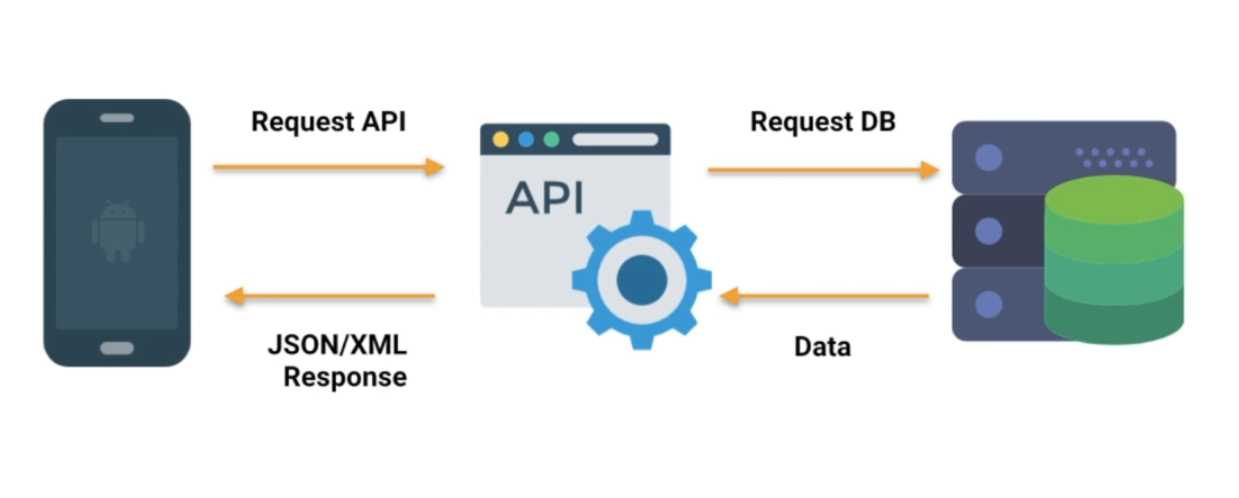
\includegraphics[width=0.9\textwidth]{Immagini/retrofit}
			\caption{Android Retrofit}
		\end{figure}
		\textbf{Firebase} è una piattaforma di sviluppo di applicazioni mobile e web fornita da Google.\\
		Offre una suite completa di strumenti e servizi progettati per aiutare gli sviluppatori a creare app di alta qualità, espanderne l'utenza e aumentare i ricavi.\\
		La piattaforma è particolarmente apprezzata per la sua capacità di semplificare molte delle operazioni necessarie per costruire, gestire e scalare le applicazioni.\\
		Le principali caratteristiche sono:
		\begin{itemize}
			\item \textbf{Realtime Database:} Un database NoSQL che consente di archiviare e sincronizzare i dati tra i client in tempo reale.
			\item Cloud Firestore: Un database flessibile, scalabile e di nuova generazione per lo sviluppo mobile, web e server.
			\item \textbf{Authentication:} Soluzioni di autenticazione per gli utenti tramite email, password e provider di terze parti come Google, Facebook e Twitter.
			\item \textbf{Hosting:} Hosting web statico veloce e sicuro per le tue app, con supporto per contenuti globalmente distribuiti tramite CDN.
			\item \textbf{Cloud Functions:} Funzionalità serverless che consentono di eseguire codice backend in risposta a eventi attivati da Firebase o richieste HTTP.
			\item \textbf{Cloud Messaging}: Un servizio che permette l'invio di notifiche push e messaggi agli utenti su diverse piattaforme.
			\item \textbf{Analytics:} Strumenti di analisi avanzati che forniscono una comprensione approfondita del comportamento degli utenti e delle prestazioni dell'app.
			\item \textbf{Crashlytics:} Un servizio di reporting in tempo reale per crash e bug, che aiuta a migliorare la stabilità dell'app.
			\item \textbf{Remote Config:} Permette di modificare dinamicamente l'aspetto e il comportamento dell'app senza rilasciare una nuova versione.
			\item \textbf{Performance Monitoring:} Monitoraggio delle prestazioni delle app in tempo reale, aiutando a identificare e risolvere i problemi di latenza e di consumo delle risorse.
		\end{itemize}
		\begin{figure}[H]
			\centering
			\includegraphics[width=0.9\textwidth]{Immagini/firebase}
			\caption{Firebase}
		\end{figure}
		\newpage
		\subsection{Class Diagram di Design}
		Per questioni di leggibilità e comprensione dei diagrammi, si è scelto di dividere il class diagram, creandone uno per ciascun package dell’applicativo.\\
		\textit{NOTA: Trattandosi di diagrammi molto ricchi, si consiglia di zoomare per poter leggere bene il contenuto in quanto potrebbe risultare poco visibile}.
		\newpage
		\subsubsection{Classi Diagram Playlist}
		\begin{figure}[H]
			\centering
			\includegraphics[width=1.0\textwidth]{Immagini/classdiagramdesignplaylist}
		\end{figure}
		\subsubsection{Class Diagram User}
		\begin{figure}[H]
			\centering
			\includegraphics[width=1.0\textwidth]{Immagini/classdiagramdesignuser}
		\end{figure}
		\subsubsection{Class Diagram Library}
		\begin{figure}[H]
			\centering
			\includegraphics[width=1.0\textwidth]{Immagini/classdiagramlibrary}
		\end{figure}
		\subsubsection{Class Diagram Listening}
		\begin{figure}[H]
			\centering
			\includegraphics[width=1.0\textwidth]{Immagini/classdiagramdesignlistening}
		\end{figure}
		\newpage
		\subsection{Sequence Diagram di design}
		Per questioni di leggibilità e comprensione dei diagrammi, si è scelto di dividere i sequence diagram.\\
		\textit{NOTA: Trattandosi di diagrammi molto ricchi, laddove sia necessario, si consiglia di zoomare per poter leggere bene il contenuto in quanto potrebbe risultare poco visibile}.
		\subsubsection{Sequence diagram Playlist}
		\begin{figure}[H]
			\centering
			\includegraphics[width=0.6\textwidth]{Immagini/sequence1}
			\caption{Parte Uno}
		\end{figure}
		\begin{figure}[H]
			\centering
			\includegraphics[width=0.8\textwidth]{Immagini/sequence2}
			\caption{Parte Due}
		\end{figure}
		\begin{figure}[H]
			\centering
			\includegraphics[width=0.8\textwidth]{Immagini/sequence3}
			\caption{Parte Tre}
		\end{figure}
		\subsubsection{Ultimo Sequence}
		\newpage
		\subsection{Gerarchie funzionali}
		La gerarchia funzionale è un metodo per organizzare e rappresentare le funzioni di un sistema in modo gerarchico. Questo approccio permette di visualizzare le relazioni tra le diverse funzioni e sottosistemi, evidenziando come si suddividono i compiti e le responsabilità.\\
		In questo paragrafo vengono rappresentate le gerarchie funzionali dell’applicativo; per semplicità sono state suddivise in due macro categorie che sono state gestite come insiemi a parte ma comunicanti in qualche modo tra di loro.
		\subsubsection{Gerarchie funzionali Login}
		\begin{figure}[H]
			\centering
			\includegraphics[width=0.9\textwidth]{Immagini/gerarchialogin}
		\end{figure}
		\subsubsection{Gerarchie funzionali Homepage}
		\begin{figure}[H]
			\centering
			\includegraphics[width=0.9\textwidth]{Immagini/gerarchiahome1}
			\caption{Gerarchia HomePage prima parte}
		\end{figure}
		\begin{figure}[H]
			\centering
			\includegraphics[width=0.9\textwidth]{Immagini/gerarchiahome2}
			\caption{Gerarchia HomePage seconda parte}
		\end{figure}
		\newpage
	\section{Codice xUnit}
	Nel contesto dello sviluppo software, l'importanza dei test unitari è fondamentale per garantire la qualità e la robustezza delle applicazioni.\\
	Nel seguente capitolo, verranno esplorati due approcci principali per il testing del software: \textbf{Black Box Testing} e \textbf{White Box Testing}. 
	Risulta essenziale comprendere il concetto di \textbf{test unitario} e il ruolo cruciale che svolgono nel processo di sviluppo.\\
	Verrà preso in considerazione l'esempio del framework JUnit, un pilastro nel mondo del testing per il linguaggio di programmazione Java. Successivamente, verranno analizzate due strategie di testing sopra citate, evidenziando le differenze chiave tra di esse e illustrando l'implementazione pratica attraverso codici di test.\\
	
	Si definisce, come primo passo, la differenza tra le due metodologie di testing:
	\begin{itemize}
		\item \textbf{Black box:}
		\begin{itemize}
			\item In questo approccio, il tester tratta il sistema come una "scatola nera", senza conoscere i dettagli interni del suo funzionamento. Il tester si concentra esclusivamente sui requisiti funzionali del sistema e sulle sue interfacce esterne.
			\item I test black box sono progettati per verificare se il sistema produce gli output desiderati dati certi input, senza preoccuparsi di come il sistema raggiunge tali output.
			\item Questo tipo di testing è utile per identificare bug, discrepanze tra requisiti e implementazione, e comportamenti imprevisti.
		\end{itemize}
		\item \textbf{White box:}
		\begin{itemize}
			\item Questo approccio si concentra invece sulle strutture interne del software, osservando il codice sorgente e i dettagli della sua implementazione.
			\item I test white box vengono progettati per esplorare il flusso di controllo del programma, il flusso di dati, e per verificare la correttezza delle strutture di dati e algoritmi.
			\item È particolarmente utile per garantire una buona copertura del codice, identificare bug logici e ottimizzare le prestazioni del software.
		\end{itemize}
	\end{itemize}
		\subsection{CODICE DI PROVA}
		\begin{lstlisting}[style=JavaStyle, caption={Il tuo codice Java}, label={lst:java_code}]
			package com.soundlab;
			
			import com.soundlab.domain.Listening;
			import com.soundlab.domain.Song;
			import com.soundlab.domain.User;
			import com.soundlab.domain.properties.SongType;
			import com.soundlab.dto.records.AddRemoveListeningDTO;
			import com.soundlab.service.ListeningService;
			import com.soundlab.utils.response.Payload;
			import org.junit.jupiter.api.Test;
			import org.springframework.beans.factory.annotation.Autowired;
			import org.springframework.boot.test.context.SpringBootTest;
			import org.springframework.boot.test.mock.mockito.MockBean;
			import org.springframework.http.HttpStatus;
			import java.util.Optional;
			
			import org.springframework.security.crypto.password.PasswordEncoder;
			import org.springframework.test.context.ContextConfiguration;
			import com.soundlab.repository.*;
			
			import static org.mockito.Mockito.*;
			import static org.junit.jupiter.api.Assertions.*;
			
			@SpringBootTest
			@ContextConfiguration(classes = SoundlabApplication.class)
			class SoundlabApplicationTests {
				
				@Autowired
				private ListeningService listeningService;
				
				@MockBean
				private UserRepository userRepository;
				
				@MockBean
				private SongRepository songRepository;
				
				@MockBean
				private ListeningRepository listeningRepository;
				
				@MockBean
				private PasswordEncoder encoder;
				
				@Test
				public void testInsertListeningSuccess() {
					// Creo e setto gli oggetti fittizzi
					User mockUser = new User();
					mockUser.setEmail("mock.user@mail.com");
					mockUser.setUsername("mockUser");
					mockUser.setPassword(encoder.encode("password"));
					Song mockSong = new Song();
					mockSong.setId(1L);
					mockSong.setTitle("mockSong");
					mockSong.setYear(2000);
					mockSong.setGenre("Genere");
					mockSong.setType(SongType.ORIGINAL);
					
					// Li cerco nei miei repositori fittizzi
					when(userRepository.findById("mock.user@mail.com")).thenReturn(Optional.of(mockUser));
					when(songRepository.findById(1L)).thenReturn(Optional.of(mockSong));
					
					AddRemoveListeningDTO dto = new AddRemoveListeningDTO("mock.user@mail.com", 1L);
					
					// Mando in esecuzione il test vero e proprio
					Payload result = listeningService.insertListening(dto);
					
					// Verifico i miei output
					assertEquals(HttpStatus.OK.value(), result.statusCode());
					assertEquals("Canzone ascoltata con successo", result.msg());
					
					// Verifico nella mia repository
					verify(userRepository).findById("mock.user@mail.com");
					verify(songRepository).findById(1L);
					verify(listeningRepository).save(any(Listening.class));
				}
			}
		\end{lstlisting}
		
		\subsection{Metodo 2}
		\subsection{Metodo 3}
		\subsection{Metodo 4}
		\newpage
	\section{Valutazione dell'usabilità sul campo}
	All'interno di quest'ultimo capitolo si analizzerà \textbf{l'usabilità sul campo} con un prodotto semi-finito.\\
	Tutto ciò è importante in quanto va ad influenzare direttamente l'esperienza dell'utente, l'efficacia operativa, la qualità del prodotto e la capacità di raggiungere un pubblico più ampio.\\
	Investire sull'usabilità è essenziale per poter creare un prodotto di successo e per poter soddisfare le esigenze dei clienti.\\
	I punti cruciali, infatti, sono:
	\begin{itemize}
		\item \textbf{Soddisfazione dell'utente:}
		\begin{itemize}
			\item Un'interfaccia utente intuitiva e facile da utilizzare migliora l'esperienza dell'utente finale e aumenta la sua soddisfazione.
			\item Gli utenti apprezzano e preferiscono prodotti e applicazioni che sono semplici e piacevoli da utilizzare.
		\end{itemize}
		\item \textbf{Efficienza operativa:}
		\begin{itemize}
			\item Un'interfaccia utente ben progettata consente agli utenti di svolgere i loro compiti in modo più rapido ed efficiente.
			\item Maggiore produttività e una riduzione dei tempi e degli sforzi necessari per completare le attività.
		\end{itemize}
		\item \textbf{Riduzione degli errori:}
		\begin{itemize}
			\item Un'interfaccia intuitiva e con feedback chiari aiuta a prevenire gli errori degli utenti durante l'utilizzo del prodotto.
			\item Ciò riduce i costi e il tempo necessario per correggere gli errori e migliorare la qualità complessiva del prodotto.
		\end{itemize}
		\item \textbf{Accessibilità e inclusività:}
		\begin{itemize}
			\item Un'interfaccia utente ben progettata è accessibile a utenti con diverse abilità, età e background.
			\item Questo aumenta l'inclusività e assicura che il prodotto possa essere utilizzato da un'ampia base di utenti.
		\end{itemize}
		\item \textbf{Adattabilità e flessibilità:}
		\begin{itemize}
			\item Un'interfaccia utente ben progettata è in grado di adattarsi a diversi contesti d'uso, dispositivi e requisiti.
			\item Ciò aumenta la versatilità e la longevità del prodotto, rendendolo più adattabile alle esigenze future.
		\end{itemize}
	\end{itemize}
		\subsection{Valutazione dell'applicativo}
		L'usabilità sul campo è stata valutata grazie a due operazioni in particolare: \textbf{valutazioni euristiche} e utilizzo dei \textbf{file di log} (trattati in seguito).\\
		Per quanto riguarda la prima, sono stati individuati tre esperti a cui sottoporre alcune domande, tenendo a mente \textbf{le 8 regole di Shneiderman}.\\
		Tali quesiti hanno come scopo quello di testare l'applicativo e trovare eventuali difetti.
		Le domande che sono state poste sono le seguenti:
		\begin{itemize}
			\item \textbf{\textit{\textcolor{dark_purple}{C'è un alto grado di usabilità universale?}}}
			\item \textbf{\textit{\textcolor{dark_purple}{Ci sono abbastanza riscontri informativi?}}}
			\item \textbf{\textit{\textcolor{dark_purple}{Gli errori sono facilmente attivabili? E se si, c'è modo di annullarli?}}}
			\item \textbf{\textit{\textcolor{dark_purple}{Il carico di memoria a breve termine è basso?}}}
			\item \textbf{\textit{\textcolor{dark_purple}{L'applicazione è grado di rispondere in tempi utili?}}}
			\item \textbf{\textit{\textcolor{dark_purple}{E' all'altezza di altri competitors?}}}
		\end{itemize}
		\subsubsection{Metodo euristico}
		Gli utilizzatori individuati hanno avuto piena libertà di esplorare l'app ma sono stati dati loro due compiti\footnote{abbiamo già fornito agli utilizzatori un profilo utente sull'applicativo, evitando cosi di dover passare per la registrazione} generali da eseguire:
		\begin{itemize}
			\item Primo compito: Creare una playlist ed inserire almeno una canzone al suo interno
			\item Secondo compito: Cercare un brano musicale ed ascoltarlo
		\end{itemize}
		Successivamente alla valutazione euristica gli stessi utenti sono stati valutati per scoprire chi è stato l’utilizzatore più attento e chi meno.\\
		I compiti assegnati sono stati eseguiti tutti in tempi brevi dai nostri valutatori. Si ha, dunque, una misura dell'usabilità abbastanza elevata che va a centrare l'obiettivo iniziale ovvero, quello di avere un grado di usabilità sul campo molto vicino a quello effettuato sui prototipi.\\
		Evitando cambiamenti durante lo sviluppo dell'app che avrebbe portato ad una maggiore quantità di tempo e risorse impiegate, si è evitato il rischio di abbassare il grado di usabilità del prodotto rispetto al prototipo, falsando ed invalidando quest'ultimo.
		\begin{figure}[H]
			\centering
			\includegraphics[width=0.9\textwidth]{Immagini/tabella}
		\end{figure}
		Come rappresentato in tabella i difetti riscontrati dagli utilizzatori sono tre.\\
		\textit{NOTA: Abbiamo voluto indicare che la creazione di una playlist sia andata a buon fine per tutti gli utilizzatori in quanto era uno dei compiti che era stato richiesto}
		
		\begin{itemize}
			\item \textbf{Bug aggiunta canzone a playlist:} 
			Quando l'utente tentava di selezionare una canzone da aggiungere alla playlist, veniva presentata una schermata che mostrava tutte le playlist create sul suo profilo. Tuttavia, in alcuni casi, l'utente non riusciva a selezionare una singola playlist specifica, il che creava problemi nell'aggiunta del brano desiderato alla playlist corretta.\\
			\textit{\textbf{Questo errore è stato risolto}}
			
			\item \textbf{Errore ricerca brano musicale:}
			Se non vengono rispettati i parametri di ricerca sviluppati dall'ingegnere del software responsabile di questa funzionalità, l'applicativo non sarà mai in grado di restituire in modo accurato la traccia musicale desiderata dall'utente finale.
			\item \textbf{Bug riproduzione brano da player:}
			Se l'utente non concede il permesso per le notifiche quando l'applicazione è in esecuzione, il player multimediale non potrà essere visualizzato nella barra delle notifiche. Di conseguenza, l'utente non sarà in grado di utilizzare il player al di fuori dell'applicazione stessa.
		\end{itemize}
		Sono stati ritenuti importanti tutti gli errori che sono stati riscontrati dagli osservatori ma, in particolare, è stata Flavia P. ad essere stata individuata come \textit{utente più attento}, in quanto è riuscita a riscontrare due problematiche che gli sviluppatori dell'applicativo risolveranno in un futuro immediato.
		Gli utilizzatori sono stati invitati a rispondere alle domande citate ad inizio paragrafo, delle quali sono state riportate le loro risposte.
		\includepdf[pages={1,2}]{Documenti/risposte.pdf}
		Grazie alle interviste condotte, il team di sviluppo ritiene di aver ottenuto risultati soddisfacenti. 
		\\Alcuni dei problemi e degli errori riscontrati sono stati già risolti, mentre per altre questioni il team si impegnerà a trovare una soluzione il prima possibile.\\
		
		Le risposte ricevute dagli utenti sono state nel complesso positive. Ciò sembra essere dovuto in parte alla fiducia accordata agli utilizzatori e ai controlli nonché alle conferme richieste durante le operazioni più critiche all'interno dell'applicazione. 
		\\Questi accorgimenti hanno contribuito a migliorare l'affidabilità percepita del sistema.
		\subsubsection{Metodo con monitoraggio}
		Grazie all’uso di Firebase è stato possibile raccogliere un gran numero di informazioni circa il gradimento dell’applicazione e le sue prestazioni.\\
		Si è fatto uso di:
		\begin{itemize}
			\item \textbf{Analytics:} per la raccolta di dati e statistiche sugli eventi all'interno dell'applicazione
			\item \textbf{Crashlytics:} per la raccolta di dati circa le interruzioni anomale dell'applicativo. Fornisce dettagli su cosa ha causato l'arresto consentendo un controllo completo dell'applicazione per assicurarne la massima stabilità
			\item \textbf{Performance:} per la raccolta di dati circa i tempi di risposta e di avvio
		\end{itemize}
	\section{Conclusione e valutazione del team}
	In questo progetto abbiamo dato vita a  \textbf{SoundLab}, una piattaforma che permette agli utenti di ascoltare e gestire la propria musica preferita in modo intuitivo e personalizzato.\\
	Attraverso l'analisi dei requisiti, la progettazione del modello funzionale e architetturale, e l'implementazione delle principali funzionalità, siamo riusciti a realizzare un'applicazione che risponde alle esigenze degli utenti target identificati.\\
	Durante lo sviluppo, abbiamo posto particolare attenzione all'esperienza utente, creando un'interfaccia grafica semplice e intuitiva che facilita la navigazione e l'interazione con le varie funzionalità. Inoltre, l'adozione di tecnologie moderne e l'architettura modulare garantiscono flessibilità e scalabilità del sistema.\\
	Nonostante i risultati raggiunti, esistono ancora numerosi margini di miglioramento e sviluppi futuri per l'applicazione.\\
	Il team pensava a tali futuri sviluppi:
	\begin{itemize}
		\item Integrazione di funzionalità avanzate di analisi dei dati e raccomandazione di brani e playlist in base alle preferenze dell'utente
		\item Implementazione di funzionalità collaborative, come la condivisione di playlist tra utenti
		\item Integrazione di funzionalità di creazione e modifica di brani musicali
		\item Implementazione di meccanismi di monetizzazione, come abbonamenti premium o vendita di contenuti aggiuntivi
	\end{itemize}
	Questi rappresentano solo alcuni degli ambiti di miglioramento e sviluppo futuro che potranno rendere SoundLab un'applicazione sempre più completa e in grado di soddisfare le esigenze degli appassionati di musica.
	\\
	Siamo estremamente soddisfatti del risultato finale del nostro lavoro. Il prodotto che abbiamo realizzato è non solo funzionale e rispondente alle esigenze degli utenti, ma anche innovativo e ben progettato.\\
	\begin{figure}[H]
		\centering
		\includegraphics[width=0.8\textwidth]{Immagini/31708}
	\end{figure}
	Abbiamo lavorato sodo come team per raggiungere questo obiettivo.
	È stato gratificante vedere il nostro lavoro prendere forma e concretizzarsi. Abbiamo affrontato diverse sfide lungo il percorso, ma grazie alla \textbf{collaborazione} e alla tenacia di tutto il team siamo riusciti a superarle.\\
	Siamo fiduciosi che il prodotto avrà un grande successo e avrà un impatto positivo sulla vita degli utenti; siamo davvero tanto entusiasti di vedere come verrà utilizzato e di come si evolverà nel tempo.\\
	Ci teniamo a specificare di quanto sia stato \textbf{stimolante} lavorare in questo team, in quanto è stata fondamentale la \textbf{collaborazione} tra noi membri. Insieme abbiamo affrontato sfide complesse, discusso diverse soluzioni e trovato il modo migliore per procedere.
	\\
	Nonostante avessimo opinioni e competenze diverse all’interno del gruppo, ciò ha portato a un processo decisionale più ricco e a soluzioni più innovative.\\
	Oltre al lavoro di squadra, riteniamo che sia stato molto formativo l'essere parte di questo team.
	\textbf{Abbiamo imparato tantissimo l’uno dagli altri}, sia per quanto riguarda le competenze tecniche che l’approccio al lavoro, delineato da tantissima \textbf{serietà} e \textbf{professionalità}.\\
	Le nostre conoscenze si sono ampliate e sono state sviluppate nuove abilità attraverso la formazione interna e la partecipazione a chiamate di “lavoro” e di “brainstorming”.\\
	In definitiva, la nostra esperienza è da valutare come positiva. 
	
		
\end{document}
